\documentclass[12pt,a4paper]{report}

\usepackage{fontspec}
\usepackage[vietnamese]{babel}
\usepackage{geometry}
\usepackage{graphicx}
\usepackage{float}
\usepackage{array}
\usepackage{amsmath}
\usepackage{longtable}
\usepackage{booktabs}
\usepackage{tabularx}
\usepackage{multirow}
\usepackage{enumitem}
\usepackage{xurl}
\usepackage{xparse}
\usepackage{hyperref}

\geometry{
    left=3cm,
    right=2cm,
    top=2.5cm,
    bottom=2.5cm
}

\setmainfont{Times New Roman}
\setsansfont{Arial}
\setmonofont{Consolas}

\graphicspath{{content/}{content/source/}}

\makeatletter
\def\input@path{{content/}}
\makeatother

\setlength{\parindent}{1.25cm}
\setlength{\parskip}{0.4em}
\renewcommand{\baselinestretch}{1.25}
\sloppy

\hypersetup{
    colorlinks=true,
    linkcolor=black,
    citecolor=black,
    urlcolor=blue
}

\begin{document}

\begin{titlepage}
    \centering
    {\Large BÁO CÁO PHÂN TÍCH KỸ THUẬT\par}
    \vspace{3cm}
    {\LARGE\bfseries Hệ thống trợ lý ảo tư vấn tuyển sinh\par}
    \vfill
    {\large \today\par}
\end{titlepage}

\tableofcontents
\clearpage

\begingroup
\let\originalchapter\chapter
\let\originalsection\section
\RenewDocumentCommand{\chapter}{s m}{%
    \originalchapter*{#2}%
    \phantomsection
    \addcontentsline{toc}{chapter}{#2}%
}
\RenewDocumentCommand{\section}{s m}{%
    \originalsection*{#2}%
    \phantomsection
    \addcontentsline{toc}{section}{#2}%
}

\chapter{GIỚI THIỆU}
\label{chap:introduction}

\section{Giới thiệu bài toán}
\label{sec:problem_introduction}
Trong bối cảnh cuộc cách mạng công nghiệp 4.0, việc ứng dụng trí tuệ nhân tạo (AI) vào mọi lĩnh vực của đời sống đã trở thành một xu hướng tất yếu, và giáo dục cũng không ngoại lệ. Hàng năm, vào mỗi mùa tuyển sinh, các cơ sở giáo dục đại học phải đối mặt với một thách thức lớn: xử lý hàng ngàn câu hỏi từ thí sinh và phụ huynh. Các câu hỏi này thường có nội dung lặp đi lặp lại, xoay quanh các chủ đề như chỉ tiêu tuyển sinh, điểm chuẩn các năm trước, các phương thức xét tuyển, thông tin học phí, chi tiết về chương trình đào tạo, và các thủ tục hành chính liên quan đến việc nhập học.

Tại Học viện Kỹ thuật Mật mã (KMA), công tác tư vấn tuyển sinh không chỉ đóng vai trò cung cấp thông tin mà còn là một kênh quan trọng để thu hút và định hướng cho các tài năng trẻ trong các lĩnh vực mũi nhọn như An toàn thông tin, Công nghệ thông tin, và Kỹ thuật Điện tử Viễn thông. Tuy nhiên, các phương pháp tư vấn truyền thống thông qua các kênh như điện thoại, email, hay các trang mạng xã hội đang dần bộc lộ những hạn chế. Việc này đòi hỏi một đội ngũ nhân sự lớn, đặc biệt là trong các giai đoạn cao điểm, dẫn đến tình trạng quá tải, phản hồi chậm trễ và đôi khi là thiếu nhất quán trong thông tin cung cấp.

Thêm vào đó, các thông tin liên quan đến tuyển sinh và quy chế đào tạo thường xuyên được cập nhật và thay đổi theo từng năm học. Việc đảm bảo rằng tất cả các tư vấn viên đều nắm bắt kịp thời và chính xác những thay đổi này là một công việc không hề đơn giản.

Từ những thực trạng trên, nhu cầu xây dựng một hệ thống trợ lý ảo thông minh, có khả năng tự động hóa việc giải đáp các thắc mắc của thí sinh một cách chính xác, nhanh chóng và liên tục 24/7 đã trở nên vô cùng cấp thiết. Hệ thống này không chỉ giúp giảm tải cho đội ngũ tư vấn viên mà còn nâng cao trải nghiệm của người dùng, cung cấp thông tin một cách tức thì và đáng tin cậy.

Nhận thức được tiềm năng to lớn của các công nghệ Xử lý Ngôn ngữ Tự nhiên (NLP) và Trí tuệ Nhân tạo, đề tài \textbf{"Nghiên cứu và xây dựng hệ thống KMA Chatbot hỗ trợ tư vấn tuyển sinh"} đã được lựa chọn. Hệ thống được đề xuất không chỉ giới hạn ở việc xử lý các kịch bản hội thoại cố định thông qua nền tảng Rasa, mà còn mở rộng khả năng của mình bằng cách tích hợp công nghệ RAG (Retrieval-Augmented Generation). Sự kết hợp này cho phép hệ thống truy xuất và tổng hợp thông tin một cách linh hoạt từ một kho tài liệu tuyển sinh đa dạng, giúp trả lời những câu hỏi phức tạp và không theo kịch bản một cách hiệu quả.

\section{Giới thiệu tài liệu}
\label{sec:document_introduction}
Tài liệu này trình bày chi tiết về quá trình phân tích, thiết kế, và triển khai hệ thống "KMA Chatbot hỗ trợ tư vấn tuyển sinh". Nội dung của tài liệu được cấu trúc một cách có hệ thống để người đọc có thể dễ dàng theo dõi và nắm bắt được toàn bộ quy trình phát triển của dự án. Cấu trúc của tài liệu bao gồm các chương chính sau:
\begin{itemize}
    \item \textbf{Giới thiệu:} Trình bày tổng quan về bài toán tư vấn tuyển sinh, bối cảnh lựa chọn đề tài và cấu trúc tài liệu.
    \item \textbf{Chương 1 - Khảo sát và phân tích yêu cầu hệ thống:} Tập trung vào việc khảo sát bài toán, xác định nhóm người dùng, phân tích yêu cầu chức năng, phi chức năng và đặc tả các ca sử dụng chính.
    \item \textbf{Chương 2 - Phân tích và thiết kế hệ thống:} Trình bày kiến trúc tổng thể, thiết kế chatbot Rasa, phân hệ RAG, API hệ thống và phân hệ quản trị.
    \item \textbf{Chương 3 - Xây dựng:} Dành cho nội dung xây dựng và triển khai hệ thống.
\end{itemize}


Qua bảng so sánh, có thể thấy với yêu cầu của một trường Đại học/Học viện về việc bảo mật thông tin, tùy biến sâu mô hình học máy và không bị phụ thuộc vào bên thứ ba (vendor lock-in), Rasa là sự lựa chọn tối ưu và bền vững nhất để làm nền tảng cốt lõi cho KMA Chatbot.


\endgroup


\chapter{KHẢO SÁT VÀ PHÂN TÍCH YÊU CẦU HỆ THỐNG}


\section{Khảo sát bài toán tư vấn tuyển sinh}
\subsection{Bối cảnh bài toán}

Tuyển sinh là một trong những hoạt động quan trọng của các trường đại học, cao đẳng và cơ sở đào tạo. Trong mỗi mùa tuyển sinh, thí sinh và phụ huynh thường có nhu cầu tìm hiểu nhiều thông tin liên quan như ngành đào tạo, mã ngành, tổ hợp xét tuyển, phương thức xét tuyển, học phí, điểm chuẩn, chỉ tiêu, thời gian đăng ký, hồ sơ cần chuẩn bị và cơ hội nghề nghiệp sau khi tốt nghiệp.

Hiện nay, các thông tin tuyển sinh thường được công bố trên nhiều kênh khác nhau như website chính thức của trường, fanpage, file PDF đề án tuyển sinh, bài viết thông báo, email, hotline hoặc các buổi tư vấn trực tiếp. Việc thông tin bị phân tán ở nhiều nguồn khiến người dùng mất nhiều thời gian tìm kiếm, đặc biệt khi họ không biết chính xác thông tin mình cần nằm ở đâu.

Bên cạnh đó, trong giai đoạn cao điểm tuyển sinh, số lượng câu hỏi gửi đến bộ phận tư vấn thường tăng mạnh. Nhiều câu hỏi có nội dung lặp lại, ví dụ như: ``Ngành Công nghệ thông tin xét tổ hợp nào?'', ``Điểm chuẩn năm trước là bao nhiêu?'', ``Trường có xét học bạ không?'', ``Học phí một năm khoảng bao nhiêu?''. Nếu toàn bộ các câu hỏi này đều được xử lý thủ công bởi cán bộ tuyển sinh, hệ thống tư vấn có thể bị quá tải, thời gian phản hồi chậm và chất lượng tư vấn không đồng đều.

Vì vậy, việc xây dựng một hệ thống chatbot tư vấn tuyển sinh có khả năng tiếp nhận câu hỏi tự nhiên, phân tích nội dung câu hỏi, truy xuất dữ liệu từ nguồn tri thức tuyển sinh và đưa ra câu trả lời phù hợp là cần thiết. Hệ thống này giúp thí sinh và phụ huynh tiếp cận thông tin nhanh hơn, đồng thời hỗ trợ nhà trường giảm tải công việc tư vấn lặp lại.

\begin{figure}[H]
    \centering
    \includegraphics[width=\textwidth]{content/source/Hình 2.1 Mô hình tư vấn tuyển sinh truyền thống và mô hình có chatbot hỗ trợ..png}
    \caption{Mô hình tư vấn tuyển sinh truyền thống và mô hình có chatbot hỗ trợ}
    \label{fig:admission_consulting_model}
\end{figure}

\subsection{Thực trạng tư vấn tuyển sinh hiện nay}

Qua khảo sát bài toán, hoạt động tư vấn tuyển sinh hiện nay thường được triển khai theo các hình thức chính sau:

Thứ nhất, người dùng tự tìm kiếm thông tin trên website chính thức của trường. Đây là nguồn dữ liệu có độ tin cậy cao, tuy nhiên thông tin thường được trình bày dưới dạng bài viết dài, bảng biểu hoặc file PDF. Người dùng phải tự đọc, tự tìm và tự đối chiếu thông tin, gây mất thời gian.

Thứ hai, người dùng đặt câu hỏi qua fanpage, email hoặc hotline. Hình thức này cho phép người dùng nhận được phản hồi từ cán bộ tuyển sinh, tuy nhiên vào mùa cao điểm, số lượng câu hỏi lớn có thể khiến thời gian phản hồi bị kéo dài. Ngoài ra, các câu hỏi lặp lại nhiều lần làm tăng khối lượng công việc cho bộ phận tư vấn.

Thứ ba, một số trường sử dụng mục câu hỏi thường gặp (FAQ). Cách này giúp người dùng tra cứu một số vấn đề phổ biến, nhưng còn hạn chế vì người dùng phải tìm đúng câu hỏi tương ứng. Nếu câu hỏi được diễn đạt khác với mẫu có sẵn, hệ thống khó hỗ trợ hiệu quả.

Thứ tư, một số chatbot truyền thống được xây dựng theo kịch bản cố định. Các chatbot này có thể xử lý các câu hỏi đơn giản nhưng thường gặp khó khăn với câu hỏi tự nhiên, câu hỏi thiếu ngữ cảnh hoặc câu hỏi yêu cầu trích xuất thông tin từ tài liệu tuyển sinh.

Từ thực trạng trên, có thể thấy bài toán tư vấn tuyển sinh cần một hệ thống có khả năng kết hợp giữa xử lý ngôn ngữ tự nhiên, quản lý hội thoại, truy xuất dữ liệu có cấu trúc và truy xuất tri thức từ tài liệu.

\begin{table}[H]
    \centering
    \caption{So sánh các hình thức tư vấn tuyển sinh hiện nay}
    \label{tab:comparison_admission_consulting_methods}
    \begin{tabular}{|p{3.4cm}|p{5.2cm}|p{5.2cm}|}
        \hline
        \textbf{Hình thức tư vấn} & \textbf{Ưu điểm} & \textbf{Hạn chế} \\ \hline
        Website trường & Chính thống, đầy đủ thông tin & Khó tìm kiếm, nhiều tài liệu dài \\ \hline
        Fanpage/Email & Có người tư vấn trực tiếp & Phản hồi chậm khi quá tải \\ \hline
        Hotline & Nhanh, trực tiếp & Phụ thuộc thời gian làm việc \\ \hline
        FAQ & Dễ triển khai & Chỉ hỗ trợ câu hỏi cố định \\ \hline
        Chatbot kịch bản & Tự động hóa một phần & Khó xử lý câu hỏi tự nhiên \\ \hline
        Chatbot Rasa + RAG & Tự động, linh hoạt, truy xuất tài liệu & Cần xây dựng dữ liệu và quản trị tri thức \\ \hline
    \end{tabular}
\end{table}

\subsection{Đặc điểm của bài toán tư vấn tuyển sinh}

Bài toán tư vấn tuyển sinh có một số đặc điểm riêng biệt so với các bài toán hỏi đáp thông thường:

Thứ nhất, thông tin tuyển sinh có tính thời vụ và thay đổi theo từng năm. Các dữ liệu như chỉ tiêu, học phí, điểm chuẩn, phương thức tuyển sinh và thời gian xét tuyển có thể được cập nhật hằng năm. Vì vậy, hệ thống cần hỗ trợ quản lý dữ liệu theo năm tuyển sinh và có cơ chế cập nhật thông tin.

Thứ hai, câu hỏi của người dùng thường ngắn, thiếu ngữ cảnh và sử dụng ngôn ngữ tự nhiên. Ví dụ: ``CNTT lấy bao nhiêu điểm?'', ``Có xét học bạ không?'', ``Học phí bao nhiêu?''. Với những câu hỏi này, hệ thống cần xác định được ý định của người dùng và các thông tin còn thiếu để hỏi lại khi cần.

Thứ ba, người dùng thường sử dụng từ viết tắt hoặc cách gọi không chính thức. Ví dụ: ``CNTT'', ``ATTT'', ``IT'', ``an toàn mạng'', ``xét học bạ'', ``khối A00''. Do đó, hệ thống cần có khả năng chuẩn hóa các cách diễn đạt này về dữ liệu chính thức trong hệ thống.

Thứ tư, nhiều câu hỏi cần truy xuất dữ liệu chính xác từ tài liệu hoặc cơ sở dữ liệu. Các câu hỏi như ``Điểm chuẩn ngành An toàn thông tin năm 2024 là bao nhiêu?'' hoặc ``Ngành Công nghệ thông tin xét những tổ hợp nào?'' cần được trả lời dựa trên nguồn dữ liệu chính thống, không nên trả lời suy đoán.

Thứ năm, một số câu hỏi mang tính tư vấn gợi ý. Ví dụ: ``Em được 24 điểm thì nên chọn ngành nào?'', ``Em học khối A01 thì có thể đăng ký ngành gì?''. Các câu hỏi này đòi hỏi hệ thống không chỉ truy xuất dữ liệu mà còn phải phân tích điều kiện của người dùng để đưa ra gợi ý phù hợp.

\begin{table}[H]
    \centering
    \caption{Một số ví dụ câu hỏi tuyển sinh và dạng xử lý tương ứng}
    \label{tab:admission_question_examples}
    \begin{tabular}{|p{4.1cm}|p{3.2cm}|p{3.1cm}|p{3.8cm}|}
        \hline
        \textbf{Câu hỏi người dùng} & \textbf{Ý định} & \textbf{Thực thể cần nhận diện} & \textbf{Hướng xử lý} \\ \hline
        CNTT xét khối nào? & Hỏi tổ hợp xét tuyển & CNTT & Tra cứu ngành và tổ hợp \\ \hline
        Điểm chuẩn ATTT 2024? & Hỏi điểm chuẩn & ATTT, 2024 & Tra cứu điểm chuẩn theo năm \\ \hline
        Trường có xét học bạ không? & Hỏi phương thức & Học bạ & Tra cứu phương thức tuyển sinh \\ \hline
        Em được 24 điểm nên chọn ngành nào? & Tư vấn ngành & 24 điểm & Gợi ý ngành phù hợp \\ \hline
        Học phí ngành CNTT bao nhiêu? & Hỏi học phí & CNTT & Tra cứu học phí \\ \hline
    \end{tabular}
\end{table}

\subsection{Mục tiêu xây dựng hệ thống}

Mục tiêu của hệ thống chatbot tư vấn tuyển sinh là xây dựng một công cụ hỗ trợ tự động, giúp người dùng tra cứu và nhận tư vấn tuyển sinh một cách nhanh chóng, chính xác và thuận tiện.

Các mục tiêu chính gồm:
\begin{itemize}
    \item Hỗ trợ người dùng đặt câu hỏi bằng ngôn ngữ tự nhiên, không cần thao tác qua nhiều menu phức tạp.
    \item Tự động nhận diện ý định và thông tin quan trọng trong câu hỏi.
    \item Cung cấp câu trả lời dựa trên dữ liệu tuyển sinh chính thống.
    \item Tích hợp hệ thống RAG để truy xuất thông tin từ tài liệu dài như đề án tuyển sinh, quy chế xét tuyển, thông báo tuyển sinh hoặc file PDF.
    \item Cung cấp phân hệ quản trị để cập nhật và kiểm soát dữ liệu (ngành học, phương thức xét tuyển, điểm chuẩn, học phí, tài liệu RAG, lịch sử hỏi đáp).
    \item Nâng cao chất lượng tư vấn và giảm tải cho cán bộ tuyển sinh thông qua tự động hóa các câu hỏi phổ biến.
\end{itemize}

\begin{figure}[H]
    \centering
    \includegraphics[width=\textwidth]{content/source/Hình 2.2 Mục tiêu tổng quát của hệ thống chatbot tuyển sinh..png}
    \caption{Mục tiêu tổng quát của hệ thống chatbot tuyển sinh}
    \label{fig:chatbot_system_objectives}
\end{figure}



\section{Phân tích đối tượng sử dụng}
Dựa trên phạm vi chức năng đã khảo sát, hệ thống chatbot tư vấn tuyển sinh gồm ba nhóm đối tượng sử dụng chính: người dùng hỏi đáp, người quản trị nội dung và người quản trị hệ thống. Ba nhóm này cùng khai thác một nền tảng chung nhưng khác nhau rõ rệt về mục tiêu sử dụng, mức độ can thiệp vào dữ liệu và quyền truy cập đến các phân hệ nghiệp vụ.

\begin{figure}[H]
    \centering
    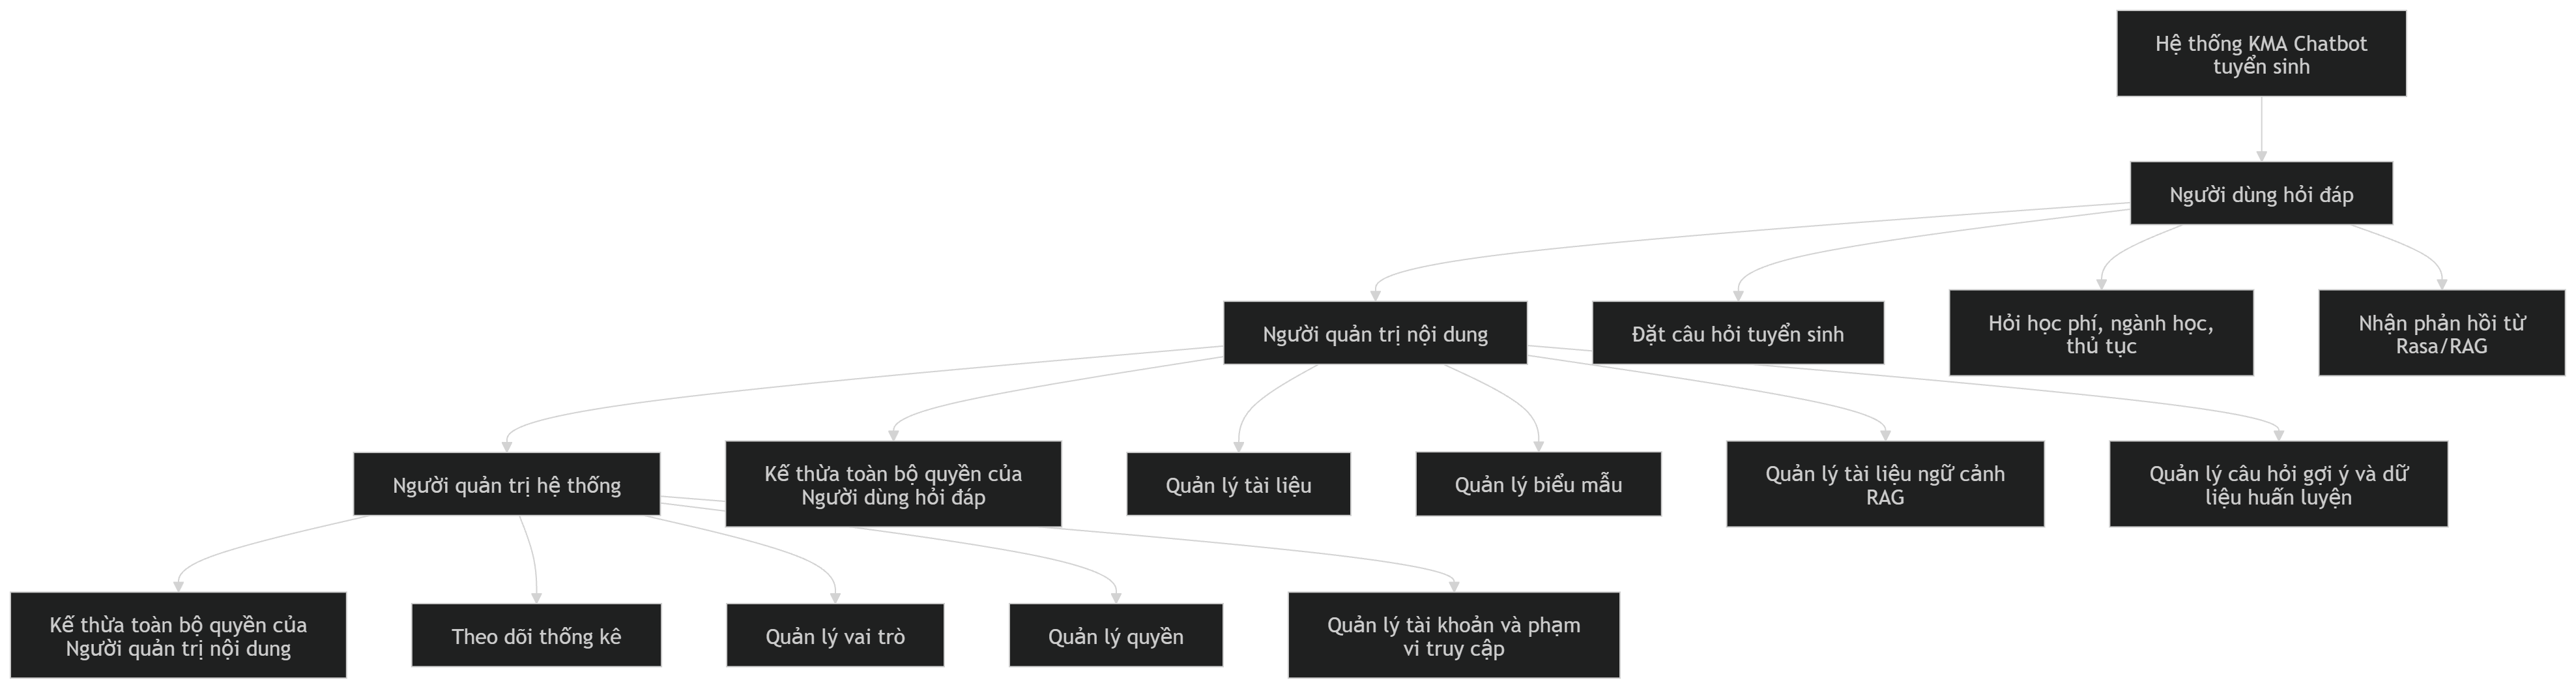
\includegraphics[width=0.8\textwidth]{content/source/User group diagram of the system.png}
    \caption{Sơ đồ các nhóm đối tượng sử dụng hệ thống}
    \label{fig:user_groups_overview}
\end{figure}

Người dùng hỏi đáp là nhóm sử dụng phổ biến nhất, tập trung vào việc đặt câu hỏi bằng ngôn ngữ tự nhiên để tra cứu thông tin tuyển sinh, ngành học, học phí, điểm chuẩn, thủ tục hoặc các biểu mẫu liên quan. Nhóm này chỉ tương tác ở mức khai thác thông tin nên không có quyền thay đổi dữ liệu, đồng thời phụ thuộc trực tiếp vào chất lượng tri thức mà hệ thống Rasa và RAG cung cấp.

Người quản trị nội dung giữ vai trò duy trì độ chính xác của kho tri thức. Họ phụ trách cập nhật tài liệu tuyển sinh, biểu mẫu, tài liệu ngữ cảnh cho RAG, câu hỏi gợi ý và một phần dữ liệu huấn luyện để chatbot luôn phản hồi đúng với quy định hiện hành. Trong khi đó, người quản trị hệ thống chịu trách nhiệm ở phạm vi rộng hơn, bao gồm quản lý tài khoản, vai trò, quyền truy cập, thống kê hoạt động và giám sát vận hành toàn bộ hệ thống.

Như vậy, sự khác biệt cốt lõi giữa ba nhóm người dùng nằm ở phạm vi thao tác: người dùng hỏi đáp chỉ khai thác thông tin, người quản trị nội dung được phép cập nhật nguồn dữ liệu phục vụ chatbot, còn người quản trị hệ thống kiểm soát hạ tầng quyền hạn và hoạt động chung. Cách phân tách này giúp hệ thống vừa hỗ trợ tư vấn thuận tiện cho người dùng cuối, vừa bảo đảm dữ liệu và vận hành được kiểm soát theo đúng trách nhiệm.

\begin{table}[H]
    \centering
    \caption{So sánh phạm vi sử dụng giữa các nhóm người dùng}
    \small
    \begin{tabularx}{\textwidth}{|p{3cm}|p{3cm}|X|p{2.5cm}|}
        \hline
        \textbf{Nhóm người dùng} & \textbf{Mục tiêu sử dụng} & \textbf{Phạm vi chức năng chính} & \textbf{Quyền thay đổi dữ liệu} \\ \hline
        Người dùng hỏi đáp & Tra cứu và nhận tư vấn tuyển sinh & Đặt câu hỏi cho chatbot, tra cứu thông tin ngành học, học phí, điểm chuẩn, thủ tục, văn bản & Không \\ \hline
        Người quản trị nội dung & Duy trì nguồn tri thức phục vụ chatbot & Quản lý tài liệu, biểu mẫu, tài liệu RAG, câu hỏi gợi ý và một phần dữ liệu huấn luyện & Có, trong phạm vi nội dung \\ \hline
        Người quản trị hệ thống & Quản lý vận hành và phân quyền & Quản lý tài khoản, vai trò, quyền truy cập, thống kê và kiểm soát hoạt động hệ thống & Có, trong phạm vi hệ thống \\ \hline
    \end{tabularx}
\end{table}



\section{Phân tích yêu cầu chức năng}

Yêu cầu chức năng mô tả các nhóm chức năng chính mà hệ thống cần cung cấp cho người dùng và người quản trị. Trong phạm vi hệ thống trợ lý ảo tuyển sinh, các chức năng được tổ chức xoay quanh hai mục tiêu chính: hỗ trợ người dùng hỏi đáp thông tin tuyển sinh và hỗ trợ quản trị viên duy trì, kiểm soát dữ liệu phục vụ chatbot.

\begin{figure}[H]
    \centering
    \includegraphics[width=\textwidth]{content/source/System_functional_decomposition_diagram.png}
    \caption{Biểu đồ phân rã chức năng hệ thống}
    \label{fig:system_functional_decomposition_diagram}
\end{figure}

Từ biểu đồ phân rã chức năng, có thể thấy hệ thống gồm các nhóm chức năng chính như hỏi đáp với chatbot, khai thác thông tin từ tài liệu, quản lý tài liệu và biểu mẫu, quản lý dữ liệu ngữ cảnh cho RAG, quản lý người dùng, phân quyền và theo dõi báo cáo thống kê. Các nhóm chức năng này liên kết với nhau để tạo thành một hệ thống vừa phục vụ hỏi đáp tự động, vừa có khả năng vận hành và cập nhật dữ liệu thường xuyên.

Đối với người dùng cuối, chức năng quan trọng nhất là đặt câu hỏi và nhận phản hồi từ chatbot. Người dùng có thể hỏi các nội dung liên quan đến ngành học, học phí, điểm chuẩn, phương thức tuyển sinh, thủ tục, biểu mẫu hoặc các thông tin chung về học viện. Với các câu hỏi phổ biến, hệ thống có thể xử lý bằng Rasa; với các câu hỏi cần dựa trên tài liệu dài hoặc văn bản đã upload, hệ thống có thể sử dụng RAG để truy xuất thông tin và tạo câu trả lời phù hợp.

Đối với nhóm quản trị, hệ thống cần hỗ trợ quản lý nguồn dữ liệu phục vụ chatbot. Các chức năng quản trị bao gồm cập nhật tài liệu, biểu mẫu, tài liệu ngữ cảnh, dữ liệu huấn luyện, câu hỏi gợi ý và theo dõi trạng thái xử lý tài liệu. Bên cạnh đó, hệ thống cũng cần có chức năng quản lý tài khoản, vai trò, quyền truy cập và báo cáo thống kê để bảo đảm quá trình vận hành được kiểm soát.

Nhìn chung, yêu cầu chức năng của hệ thống không chỉ dừng lại ở việc trả lời câu hỏi tuyển sinh, mà còn bao gồm các công cụ quản trị cần thiết để duy trì chất lượng dữ liệu, theo dõi hoạt động và phân quyền sử dụng. Đây là cơ sở để hệ thống có thể vận hành ổn định trong môi trường thực tế, nơi thông tin tuyển sinh và tài liệu liên quan thường xuyên thay đổi.



\section{Phân tích yêu cầu phi chức năng}

Yêu cầu phi chức năng mô tả các tiêu chí chất lượng mà hệ thống cần đáp ứng trong quá trình vận hành. Nếu yêu cầu chức năng trả lời câu hỏi hệ thống cần làm gì, thì yêu cầu phi chức năng tập trung vào cách hệ thống hoạt động sao cho ổn định, tin cậy, an toàn và phù hợp với môi trường sử dụng thực tế.

\begin{figure}[H]
    \centering
    \includegraphics[width=0.9\textwidth]{content/source/The groups require non-functional systems.png}
    \caption{Các nhóm yêu cầu phi chức năng của hệ thống}
    \label{fig:non_functional_groups}
\end{figure}

Đối với hệ thống trợ lý ảo tuyển sinh, yêu cầu phi chức năng có vai trò quan trọng vì hệ thống xử lý các thông tin có ảnh hưởng trực tiếp đến người dùng như ngành đào tạo, học phí, điểm chuẩn, thủ tục, biểu mẫu và quy chế tuyển sinh. Do đó, hệ thống cần ưu tiên tính chính xác, hạn chế trả lời theo suy đoán và có khả năng dựa trên nguồn dữ liệu đã được quản lý.

Hệ thống cần bảo đảm câu trả lời có căn cứ, đặc biệt với các câu hỏi sử dụng RAG. Khi người dùng hỏi về thông tin nằm trong tài liệu, hệ thống phải truy xuất nội dung liên quan trước khi sinh câu trả lời. Nếu không tìm thấy dữ liệu phù hợp, chatbot nên phản hồi rằng chưa đủ thông tin thay vì tự tạo ra nội dung không có trong nguồn tài liệu.

Bên cạnh tính đúng nguồn, hệ thống cũng cần có khả năng truy vết và vận hành ổn định. Tài liệu đưa vào hệ thống cần có trạng thái xử lý rõ ràng để quản trị viên biết tài liệu nào đã sẵn sàng sử dụng, tài liệu nào đang chờ xử lý và tài liệu nào bị lỗi. Các thao tác như upload, scan, retry pipeline, refresh dữ liệu và theo dõi thống kê giúp việc vận hành hệ thống thuận tiện hơn.

Về bảo mật, hệ thống cần phân quyền rõ ràng giữa người dùng thông thường, người quản lý và admin. Người dùng thông thường chỉ nên được sử dụng các chức năng hỏi đáp và tra cứu; trong khi đó, các chức năng quản lý tài liệu, quản lý người dùng, phân quyền và xem thống kê cần được giới hạn cho các tài khoản có quyền phù hợp. Điều này giúp bảo vệ dữ liệu và tránh các thay đổi ngoài phạm vi trách nhiệm.

Ngoài ra, hệ thống cần có khả năng mở rộng khi số lượng người dùng, tài liệu và câu hỏi tăng lên. Việc tách các thành phần như lưu trữ tài liệu, trạng thái xử lý, vector database và dữ liệu quản trị giúp hệ thống dễ nâng cấp hơn trong tương lai. Nhìn chung, các yêu cầu phi chức năng giúp hệ thống không chỉ đáp ứng được nghiệp vụ hỏi đáp, mà còn có đủ độ tin cậy để triển khai và vận hành lâu dài.


% 
\section{Phân tích yêu cầu đối với trợ lý ảo tuyển sinh}

Trợ lý ảo tuyển sinh là thành phần trực tiếp tương tác với người dùng. Thành phần này cần có khả năng hiểu câu hỏi, quản lý hội thoại, lựa chọn nguồn dữ liệu phù hợp và trả lời bằng ngôn ngữ tự nhiên.

\subsection{Yêu cầu về hiểu ngôn ngữ tự nhiên}
\begin{table}[H]
\centering
\caption{Các intent chính của trợ lý ảo}
\label{tab:intents_main}
\begin{tabular}{|p{4.2cm}|p{7.8cm}|}
\hline
\textbf{Intent} & \textbf{Mô tả} \\ \hline
ask\_major\_info & Hỏi thông tin ngành học \\ \hline
ask\_admission\_method & Hỏi phương thức tuyển sinh \\ \hline
ask\_subject\_combination & Hỏi tổ hợp xét tuyển \\ \hline
ask\_benchmark\_score & Hỏi điểm chuẩn \\ \hline
ask\_tuition\_fee & Hỏi học phí \\ \hline
ask\_quota & Hỏi chỉ tiêu \\ \hline
ask\_admission\_time & Hỏi thời gian tuyển sinh \\ \hline
ask\_profile\_document & Hỏi hồ sơ xét tuyển \\ \hline
ask\_contact & Hỏi thông tin liên hệ \\ \hline
ask\_career\_opportunity & Hỏi cơ hội nghề nghiệp \\ \hline
ask\_recommend\_major & Hỏi gợi ý ngành học \\ \hline
out\_of\_scope & Câu hỏi ngoài phạm vi \\ \hline
\end{tabular}
\end{table}

\subsection{Yêu cầu về trích xuất thực thể}
\begin{table}[H]
\centering
\caption{Các thực thể cần trích xuất}
\label{tab:entities_main}
\begin{tabular}{|p{3.2cm}|p{8.8cm}|}
\hline
\textbf{Entity} & \textbf{Ví dụ} \\ \hline
major & Công nghệ thông tin, An toàn thông tin, CNTT, ATTT \\ \hline
year & 2023, 2024, năm ngoái, năm nay \\ \hline
subject\_group & A00, A01, D01 \\ \hline
score & 23 điểm, 24.5 điểm \\ \hline
admission\_method & xét học bạ, xét điểm thi THPT \\ \hline
tuition\_type & học phí, lệ phí, học bổng \\ \hline
time\_type & hạn nộp hồ sơ, thời gian nhập học \\ \hline
\end{tabular}
\end{table}

\subsection{Yêu cầu về quản lý hội thoại}
\begin{itemize}
    \item Người dùng hỏi: ``Ngành Công nghệ thông tin xét khối nào?''
    \item Chatbot trả lời danh sách tổ hợp xét tuyển.
    \item Người dùng hỏi tiếp: ``Điểm chuẩn năm ngoái bao nhiêu?''
\end{itemize}

Hệ thống cần hiểu rằng ``năm ngoái'' đang hỏi tiếp về ngành Công nghệ thông tin. Do đó, chatbot cần lưu tạm các thông tin như ngành đang được hỏi, năm tuyển sinh, phương thức xét tuyển hoặc tổ hợp môn trong phiên hội thoại.

\subsection{Yêu cầu về xử lý fallback}
\begin{table}[H]
\centering
\caption{Các tình huống fallback và hướng xử lý}
\label{tab:fallback_cases}
\begin{tabular}{|p{4.4cm}|p{7.6cm}|}
\hline
\textbf{Trường hợp} & \textbf{Cách xử lý} \\ \hline
Không nhận diện được intent & Gợi ý người dùng hỏi lại rõ hơn \\ \hline
Thiếu tên ngành & Hỏi người dùng muốn hỏi ngành nào \\ \hline
Thiếu năm & Hỏi người dùng muốn xem năm nào \\ \hline
Không có dữ liệu & Thông báo chưa có thông tin và gợi ý liên hệ \\ \hline
Câu hỏi ngoài phạm vi & Lịch sự từ chối và hướng về tuyển sinh \\ \hline
\end{tabular}
\end{table}

\begin{figure}[H]
    \centering
    \includegraphics[width=\textwidth]{content/source/Hình 2.4 Luồng xử lý câu hỏi của trợ lý ảo..png}
    \caption{Luồng xử lý câu hỏi của trợ lý ảo}
    \label{fig:virtual_assistant_flow}
\end{figure}


% 
\section{Phân tích yêu cầu đối với hệ thống RAG}

RAG (Retrieval-Augmented Generation) là kỹ thuật kết hợp giữa truy xuất thông tin và sinh câu trả lời bằng mô hình ngôn ngữ.

\subsection{Vai trò của RAG trong hệ thống}
\begin{table}[H]
\centering
\caption{Vai trò của RAG}
\label{tab:rag_roles}
\begin{tabular}{|p{4cm}|p{8cm}|}
\hline
\textbf{Vai trò} & \textbf{Mô tả} \\ \hline
Truy xuất tài liệu & Tìm đoạn nội dung liên quan đến câu hỏi \\ \hline
Bổ sung tri thức & Hỗ trợ các câu hỏi không nằm trong intent cố định \\ \hline
Giảm trả lời sai & Câu trả lời dựa trên bằng chứng tìm được \\ \hline
Hỗ trợ trích dẫn & Cho phép hiển thị nguồn tham khảo \\ \hline
Dễ cập nhật & Chỉ cần upload tài liệu mới và index lại \\ \hline
\end{tabular}
\end{table}

\subsection{Yêu cầu đối với dữ liệu đầu vào}
\begin{table}[H]
\centering
\caption{Yêu cầu đối với dữ liệu RAG đầu vào}
\label{tab:rag_input_requirements}
\begin{tabular}{|p{4cm}|p{8cm}|}
\hline
\textbf{Yêu cầu} & \textbf{Mô tả} \\ \hline
Nguồn chính thống & Tài liệu lấy từ trường hoặc đơn vị tuyển sinh \\ \hline
Định dạng hỗ trợ & PDF, DOCX, TXT, HTML hoặc văn bản thuần \\ \hline
Nội dung rõ ràng & Có tiêu đề, mục lục, bảng biểu nếu cần \\ \hline
Có thông tin năm & Tài liệu nên gắn với năm tuyển sinh \\ \hline
Được kiểm duyệt & Quản trị viên cần xác nhận trước khi sử dụng \\ \hline
\end{tabular}
\end{table}

\subsection{Yêu cầu đối với quá trình indexing}
\begin{enumerate}
    \item Upload tài liệu.
    \item Trích xuất văn bản từ tài liệu.
    \item Làm sạch nội dung.
    \item Chia văn bản thành các đoạn nhỏ.
    \item Gắn metadata cho từng đoạn.
    \item Sinh embedding.
    \item Lưu vào vector store.
    \item Lưu thông tin tài liệu vào document store.
\end{enumerate}

\begin{figure}[H]
    \centering
    \includegraphics[width=\textwidth]{content/source/Hình 2.5 Luồng Indexing Flow của hệ thống RAG..png}
    \caption{Luồng indexing của hệ thống RAG}
    \label{fig:rag_indexing_flow}
\end{figure}

\subsection{Yêu cầu đối với quá trình truy vấn}
\begin{enumerate}
    \item Nhận câu hỏi từ chatbot.
    \item Chuẩn hóa câu hỏi.
    \item Sinh embedding cho câu hỏi.
    \item Truy xuất các đoạn liên quan từ vector store.
    \item Có thể tái xếp hạng kết quả nếu cần.
    \item Tạo prompt gồm câu hỏi và bằng chứng.
    \item Gọi mô hình sinh câu trả lời.
    \item Trả lời người dùng kèm nguồn tham khảo.
\end{enumerate}

\begin{figure}[H]
    \centering
    \includegraphics[width=\textwidth]{content/source/Hình 2.6 Luồng Query Flow của hệ thống RAG.png}
    \caption{Luồng truy vấn của hệ thống RAG}
    \label{fig:rag_query_flow}
\end{figure}

\subsection{Yêu cầu về metadata}
\begin{table}[H]
\centering
\caption{Metadata đề xuất cho mỗi đoạn tài liệu}
\label{tab:rag_metadata}
\begin{tabular}{|p{3.6cm}|p{8.4cm}|}
\hline
\textbf{Metadata} & \textbf{Ý nghĩa} \\ \hline
document\_id & Mã tài liệu \\ \hline
document\_name & Tên tài liệu \\ \hline
year & Năm tuyển sinh \\ \hline
source\_type & Loại tài liệu: đề án, thông báo, quy chế \\ \hline
page\_number & Số trang \\ \hline
section\_title & Tiêu đề mục \\ \hline
created\_at & Thời điểm thêm vào hệ thống \\ \hline
status & Trạng thái: đang dùng, nháp, đã khóa \\ \hline
\end{tabular}
\end{table}

\subsection{Yêu cầu về chất lượng RAG}
\begin{table}[H]
\centering
\caption{Yêu cầu chất lượng cho hệ thống RAG}
\label{tab:rag_quality}
\begin{tabular}{|p{2.2cm}|p{9.8cm}|}
\hline
\textbf{Mã} & \textbf{Nội dung} \\ \hline
RAG-01 & Truy xuất đúng đoạn liên quan đến câu hỏi \\ \hline
RAG-02 & Ưu tiên tài liệu mới nhất hoặc đúng năm người dùng hỏi \\ \hline
RAG-03 & Câu trả lời phải dựa trên bằng chứng truy xuất \\ \hline
RAG-04 & Không sinh câu trả lời nếu không tìm thấy bằng chứng phù hợp \\ \hline
RAG-05 & Có thể hiển thị nguồn tài liệu để người dùng kiểm tra \\ \hline
RAG-06 & Hỗ trợ cập nhật hoặc xóa tài liệu lỗi thời \\ \hline
RAG-07 & Cho phép quản trị viên index lại tài liệu khi có thay đổi \\ \hline
\end{tabular}
\end{table}


% 
\section{Phân tích yêu cầu đối với phân hệ quản trị}

Phân hệ quản trị đóng vai trò quan trọng trong việc duy trì độ chính xác và tính cập nhật của hệ thống.

\subsection{Vai trò của phân hệ quản trị}
\begin{table}[H]
\centering
\caption{Vai trò chính của phân hệ quản trị}
\label{tab:admin_module_roles}
\begin{tabular}{|p{4cm}|p{8cm}|}
\hline
\textbf{Vai trò} & \textbf{Mô tả} \\ \hline
Quản lý dữ liệu tuyển sinh & Cập nhật ngành, điểm chuẩn, học phí, chỉ tiêu \\ \hline
Quản lý tài liệu RAG & Upload, xóa, index lại tài liệu \\ \hline
Quản lý câu hỏi & Theo dõi lịch sử hỏi đáp \\ \hline
Cải thiện chatbot & Xem câu hỏi chưa trả lời được để bổ sung dữ liệu \\ \hline
Quản lý người dùng quản trị & Phân quyền, bảo mật truy cập \\ \hline
Thống kê hiệu quả & Theo dõi số lượt hỏi, intent phổ biến \\ \hline
\end{tabular}
\end{table}

\subsection{Các chức năng quản trị dữ liệu tuyển sinh}
\begin{table}[H]
\centering
\caption{Các chức năng quản trị dữ liệu tuyển sinh}
\label{tab:admin_data_functions}
\begin{tabular}{|p{4cm}|p{8cm}|}
\hline
\textbf{Nhóm dữ liệu} & \textbf{Chức năng} \\ \hline
Ngành đào tạo & Thêm, sửa, xóa, tìm kiếm ngành \\ \hline
Tổ hợp xét tuyển & Gán tổ hợp cho từng ngành \\ \hline
Điểm chuẩn & Cập nhật điểm chuẩn theo năm \\ \hline
Chỉ tiêu & Cập nhật chỉ tiêu theo ngành, theo năm \\ \hline
Học phí & Cập nhật học phí theo ngành/chương trình \\ \hline
Phương thức xét tuyển & Quản lý xét điểm thi, học bạ, xét tuyển thẳng \\ \hline
FAQ & Quản lý câu hỏi thường gặp \\ \hline
\end{tabular}
\end{table}

\subsection{Các chức năng quản trị tài liệu RAG}
\begin{table}[H]
\centering
\caption{Các chức năng quản trị tài liệu RAG}
\label{tab:admin_rag_functions}
\begin{tabular}{|p{4cm}|p{8cm}|}
\hline
\textbf{Chức năng} & \textbf{Mô tả} \\ \hline
Upload tài liệu & Tải lên file PDF, DOCX, TXT \\ \hline
Xem danh sách tài liệu & Hiển thị tên, loại, năm, trạng thái \\ \hline
Xóa tài liệu & Loại bỏ tài liệu không còn sử dụng \\ \hline
Index tài liệu & Xử lý tài liệu để đưa vào vector store \\ \hline
Re-index tài liệu & Xử lý lại khi tài liệu thay đổi \\ \hline
Xem chunk & Kiểm tra các đoạn văn bản sau khi chia \\ \hline
Bật/tắt trạng thái sử dụng & Kiểm soát tài liệu nào được dùng để trả lời \\ \hline
\end{tabular}
\end{table}

\subsection{Theo dõi lịch sử hỏi đáp}
\begin{table}[H]
\centering
\caption{Các trường dữ liệu lịch sử hỏi đáp}
\label{tab:qa_history_fields}
\begin{tabular}{|p{3.6cm}|p{8.4cm}|}
\hline
\textbf{Trường dữ liệu} & \textbf{Ý nghĩa} \\ \hline
question & Câu hỏi người dùng \\ \hline
answer & Câu trả lời của chatbot \\ \hline
intent & Ý định được nhận diện \\ \hline
entities & Các thực thể trích xuất được \\ \hline
source & Nguồn trả lời: CSDL, RAG, fallback \\ \hline
confidence & Độ tin cậy nếu có \\ \hline
created\_at & Thời gian hỏi \\ \hline
user\_feedback & Đánh giá của người dùng \\ \hline
\end{tabular}
\end{table}

\subsection{Thống kê và báo cáo}
\begin{table}[H]
\centering
\caption{Các chỉ số thống kê cần theo dõi}
\label{tab:admin_statistics}
\begin{tabular}{|p{4cm}|p{8cm}|}
\hline
\textbf{Thống kê} & \textbf{Ý nghĩa} \\ \hline
Tổng số lượt hỏi & Đánh giá mức độ sử dụng \\ \hline
Số câu hỏi theo ngày & Theo dõi cao điểm tuyển sinh \\ \hline
Intent phổ biến & Biết người dùng quan tâm nhiều đến nội dung nào \\ \hline
Câu hỏi fallback & Phát hiện lỗ hổng tri thức \\ \hline
Tài liệu được truy xuất nhiều & Đánh giá nguồn tri thức quan trọng \\ \hline
Tỷ lệ phản hồi thành công & Đánh giá hiệu quả chatbot \\ \hline
\end{tabular}
\end{table}

\begin{figure}[H]
    \centering
    \includegraphics[width=\textwidth]{content/source/Hình 2.7 Luồng quản trị dữ liệu và cải thiện chatbot..png}
    \caption{Luồng quản trị dữ liệu và cải thiện chatbot}
    \label{fig:admin_improvement_flow}
\end{figure}

.

\section{Biểu đồ Use Case tổng thể}

Biểu đồ Use Case tổng thể được sử dụng để mô tả các tác nhân tham gia hệ thống và các nhóm chức năng chính mà từng tác nhân có thể thực hiện. Dựa trên phạm vi triển khai, hệ thống trợ lý ảo tuyển sinh gồm bốn vai trò chính: Khách, Người dùng, Quản lý và Admin.

\subsection{Danh sách tác nhân}
\begin{table}[H]
\centering
\caption{Danh sách tác nhân trong hệ thống}
\label{tab:actors_list}
\begin{tabular}{|p{3.2cm}|p{6.8cm}|p{5cm}|}
\hline
\textbf{Tác nhân} & \textbf{Mô tả} & \textbf{Phạm vi sử dụng} \\ \hline
Khách & Là người truy cập hệ thống khi chưa đăng nhập, có nhu cầu hỏi đáp nhanh với trợ lý ảo & Hỏi đáp với Rasa \\ \hline
Người dùng & Là người sử dụng hệ thống sau khi đăng nhập để hỏi đáp và theo dõi thông tin hội thoại của bản thân & Hỏi đáp với Rasa, quản lý lịch sử hội thoại \\ \hline
Quản lý & Là người phụ trách vận hành dữ liệu nghiệp vụ, tài liệu, biểu mẫu, bộ dữ liệu và các cấu hình phục vụ chatbot & Quản lý bộ dữ liệu, văn bản biểu mẫu, bộ API, người dùng theo phạm vi được cấp quyền \\ \hline
Admin & Là người quản trị cấp cao, chịu trách nhiệm phân quyền, quản trị người dùng và theo dõi báo cáo thống kê toàn hệ thống & Quản lý người dùng, vai trò, quyền hạn và báo cáo thống kê \\ \hline
\end{tabular}
\end{table}

\subsection{Danh sách Use Case tổng thể}

\begin{table}[H]
\centering
\caption{Danh sách Use Case tổng thể}
\label{tab:usecase_list}
\begin{tabular}{|p{1.5cm}|p{4.2cm}|p{3cm}|p{6.3cm}|}
\hline
\textbf{Mã Use Case} & \textbf{Tên Use Case} & \textbf{Tác nhân chính} & \textbf{Mô tả} \\ \hline
UC-01 & Hỏi đáp với Rasa & Khách, Người dùng & Tác nhân đặt câu hỏi tuyển sinh và nhận phản hồi từ trợ lý ảo Rasa \\ \hline
UC-02 & Đăng nhập & Người dùng, Quản lý, Admin & Xác thực tài khoản trước khi sử dụng các chức năng cần phân quyền \\ \hline
UC-03 & Quản lý lịch sử hội thoại & Người dùng & Xem và quản lý các hội thoại đã thực hiện với chatbot \\ \hline
UC-04 & Quản lý các bộ dữ liệu & Quản lý & Thêm, xem chi tiết, thu thập dữ liệu và quản lý câu hỏi gợi ý \\ \hline
UC-05 & Quản lý văn bản, biểu mẫu & Quản lý & Quản lý văn bản và tài liệu ngữ cảnh phục vụ tra cứu, hỏi đáp \\ \hline
UC-06 & Quản lý bộ API & Quản lý & Quản lý các API hoặc tài liệu API phục vụ tích hợp hệ thống \\ \hline
UC-07 & Quản lý chatbot Rasa & Admin & Quản lý intent, entity, action, response, rule, story, slot và cấu hình chatbot \\ \hline
UC-08 & Quản lý người dùng & Quản lý, Admin & CRUD người dùng, ban/unban, thiết lập vai trò và cấp chatbot \\ \hline
UC-09 & Quản lý vai trò và quyền hạn & Admin & Quản lý vai trò, quyền hạn, gán quyền cho vai trò và gán vai trò cho người dùng \\ \hline
UC-10 & Báo cáo thống kê & Admin & Xem thống kê người dùng, hội thoại, chatbot, NLP và văn bản \\ \hline
\end{tabular}
\end{table}

\subsection{Mô tả quan hệ giữa các Use Case}

Các Use Case dành cho Người dùng, Quản lý và Admin đều cần thực hiện đăng nhập trước khi truy cập chức năng tương ứng. Vai trò Khách chỉ sử dụng chức năng hỏi đáp cơ bản với Rasa; khi cần lưu lịch sử hoặc dùng các chức năng cá nhân, Khách có thể chuyển thành Người dùng sau khi đăng nhập.

Nhóm chức năng của Quản lý tập trung vào dữ liệu nghiệp vụ, văn bản, biểu mẫu, bộ dữ liệu và bộ API. Nhóm chức năng của Admin tập trung vào quản trị quyền hạn, người dùng, chatbot Rasa và báo cáo thống kê. Cách phân tách này giúp hệ thống kiểm soát rõ phạm vi thao tác giữa người vận hành nội dung và người quản trị cấp cao.

\subsection{Biểu đồ Use Case tổng thể và phân rã}

\begin{figure}[H]
    \centering
    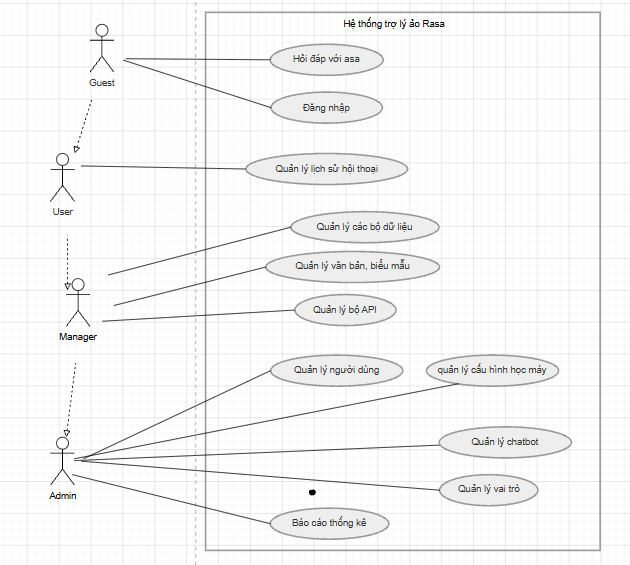
\includegraphics[width=\textwidth]{content/source/usecase/tong_quat.png}
    \caption{Biểu đồ Use Case tổng thể của hệ thống}
    \label{fig:overall_use_case}
\end{figure}

\begin{figure}[H]
    \centering
    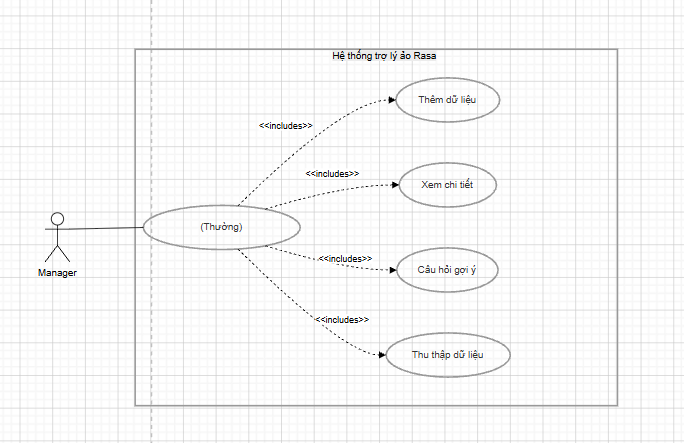
\includegraphics[width=0.92\textwidth]{content/source/usecase/quan ly thuong.png}
    \caption{Biểu đồ phân rã Use Case quản lý thường}
    \label{fig:usecase_decomposition_common}
\end{figure}

\begin{figure}[H]
    \centering
    \includegraphics[width=\textwidth]{content/source/usecase/quản lý chuyên gia.png}
    \caption{Biểu đồ phân rã Use Case quản lý chatbot Rasa}
    \label{fig:usecase_decomposition_rasa_chatbot}
\end{figure}

\begin{figure}[H]
    \centering
    \includegraphics[width=0.95\textwidth]{content/source/usecase/quản lý người dùng.png}
    \caption{Biểu đồ phân rã Use Case quản lý người dùng}
    \label{fig:usecase_decomposition_users}
\end{figure}

\begin{figure}[H]
    \centering
    \includegraphics[width=0.95\textwidth]{content/source/usecase/quản lý văn bản biểu mẫu.png}
    \caption{Biểu đồ phân rã Use Case quản lý văn bản, biểu mẫu}
    \label{fig:usecase_decomposition_documents_forms}
\end{figure}

\begin{figure}[H]
    \centering
    \includegraphics[width=0.95\textwidth]{content/source/usecase/Quản lý RABC.png}
    \caption{Biểu đồ phân rã Use Case quản lý vai trò và quyền hạn}
    \label{fig:usecase_decomposition_rbac}
\end{figure}

\begin{figure}[H]
    \centering
    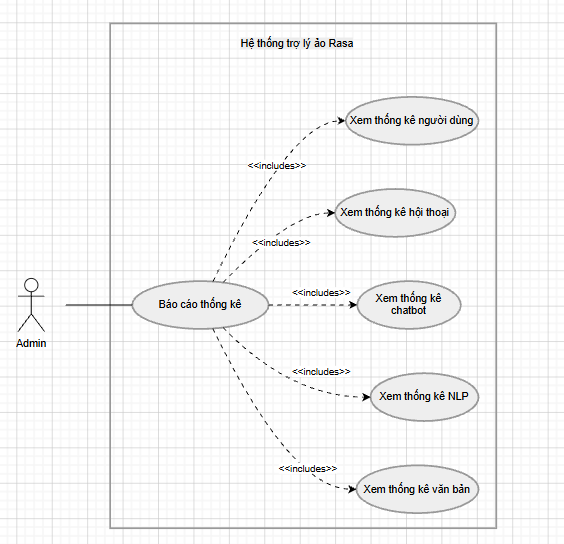
\includegraphics[width=0.8\textwidth]{content/source/usecase/bao_cao_thong_ke.png}
    \caption{Biểu đồ phân rã Use Case báo cáo thống kê}
    \label{fig:usecase_decomposition_statistics}
\end{figure}



\section{Đặc tả các Use Case chính}

\subsection{UC-01: Hỏi thông tin tuyển sinh}
\begin{table}[H]
\centering
\begin{tabular}{|p{3.5cm}|p{8.5cm}|}
\hline
\textbf{Thành phần} & \textbf{Mô tả} \\ \hline
Mã Use Case & UC-01 \\ \hline
Tên Use Case & Hỏi thông tin tuyển sinh \\ \hline
Tác nhân & Thí sinh, Phụ huynh \\ \hline
Mục tiêu & Người dùng đặt câu hỏi và nhận câu trả lời từ chatbot \\ \hline
Tiền điều kiện & Người dùng truy cập được giao diện chatbot \\ \hline
Hậu điều kiện & Câu hỏi và câu trả lời được lưu vào lịch sử \\ \hline
Luồng chính & 1) Người dùng nhập câu hỏi; 2) Hệ thống tiếp nhận; 3) Chatbot phân tích intent và entity; 4) Truy xuất dữ liệu phù hợp; 5) Trả lời người dùng \\ \hline
Luồng thay thế & Nếu thiếu thông tin, chatbot hỏi lại người dùng \\ \hline
Ngoại lệ & Nếu không tìm thấy dữ liệu, chatbot thông báo chưa có thông tin phù hợp \\ \hline
\end{tabular}
\end{table}

\subsection{UC-02: Tra cứu ngành đào tạo}
\begin{table}[H]
\centering
\begin{tabular}{|p{3.5cm}|p{8.5cm}|}
\hline
\textbf{Thành phần} & \textbf{Mô tả} \\ \hline
Mã Use Case & UC-02 \\ \hline
Tên Use Case & Tra cứu ngành đào tạo \\ \hline
Tác nhân & Thí sinh, Phụ huynh \\ \hline
Mục tiêu & Người dùng xem thông tin chi tiết về ngành học \\ \hline
Tiền điều kiện & Dữ liệu ngành đã được cập nhật \\ \hline
Hậu điều kiện & Thông tin ngành được hiển thị cho người dùng \\ \hline
Luồng chính & 1) Người dùng hỏi về ngành; 2) Nhận diện tên ngành; 3) Truy vấn CSDL ngành; 4) Trả lời thông tin ngành \\ \hline
Luồng thay thế & Nếu tên ngành chưa rõ, chatbot gợi ý danh sách ngành gần đúng \\ \hline
Ngoại lệ & Nếu ngành không tồn tại, chatbot thông báo không tìm thấy \\ \hline
\end{tabular}
\end{table}

\subsection{UC-03: Tra cứu điểm chuẩn}
\begin{table}[H]
\centering
\begin{tabular}{|p{3.5cm}|p{8.5cm}|}
\hline
\textbf{Thành phần} & \textbf{Mô tả} \\ \hline
Mã Use Case & UC-03 \\ \hline
Tên Use Case & Tra cứu điểm chuẩn \\ \hline
Tác nhân & Thí sinh, Phụ huynh \\ \hline
Mục tiêu & Người dùng xem điểm chuẩn của ngành theo năm \\ \hline
Tiền điều kiện & Dữ liệu điểm chuẩn đã được nhập \\ \hline
Hậu điều kiện & Điểm chuẩn được hiển thị \\ \hline
Luồng chính & 1) Người dùng hỏi điểm chuẩn; 2) Nhận diện ngành và năm; 3) Truy vấn điểm chuẩn; 4) Trả lời \\ \hline
Luồng thay thế & Nếu thiếu năm, mặc định năm gần nhất hoặc hỏi lại người dùng \\ \hline
Ngoại lệ & Nếu chưa có dữ liệu điểm chuẩn, chatbot thông báo chưa cập nhật \\ \hline
\end{tabular}
\end{table}

\subsection{UC-04: Tra cứu học phí}
\begin{table}[H]
\centering
\begin{tabular}{|p{3.5cm}|p{8.5cm}|}
\hline
\textbf{Thành phần} & \textbf{Mô tả} \\ \hline
Mã Use Case & UC-04 \\ \hline
Tên Use Case & Tra cứu học phí \\ \hline
Tác nhân & Thí sinh, Phụ huynh \\ \hline
Mục tiêu & Người dùng xem học phí theo ngành hoặc chương trình \\ \hline
Tiền điều kiện & Dữ liệu học phí đã được cập nhật \\ \hline
Hậu điều kiện & Học phí được hiển thị cho người dùng \\ \hline
Luồng chính & 1) Người dùng hỏi học phí; 2) Nhận diện ngành (nếu có); 3) Truy vấn dữ liệu học phí; 4) Trả lời \\ \hline
Luồng thay thế & Nếu người dùng hỏi học phí chung, hệ thống trả lời mức học phí tổng quan \\ \hline
Ngoại lệ & Nếu chưa có học phí ngành đó, chatbot gợi ý liên hệ phòng tuyển sinh \\ \hline
\end{tabular}
\end{table}

\subsection{UC-05: Nhận gợi ý ngành học}
\begin{table}[H]
\centering
\begin{tabular}{|p{3.5cm}|p{8.5cm}|}
\hline
\textbf{Thành phần} & \textbf{Mô tả} \\ \hline
Mã Use Case & UC-05 \\ \hline
Tên Use Case & Nhận gợi ý ngành học \\ \hline
Tác nhân & Thí sinh \\ \hline
Mục tiêu & Gợi ý ngành phù hợp dựa trên điểm số, tổ hợp hoặc sở thích \\ \hline
Tiền điều kiện & Có dữ liệu ngành, điểm chuẩn, tổ hợp xét tuyển \\ \hline
Hậu điều kiện & Danh sách ngành gợi ý được hiển thị \\ \hline
Luồng chính & 1) Người dùng nhập điểm/tổ hợp; 2) Hệ thống phân tích; 3) Lọc ngành phù hợp; 4) Trả danh sách gợi ý \\ \hline
Luồng thay thế & Nếu thiếu điểm hoặc tổ hợp, chatbot hỏi lại \\ \hline
Ngoại lệ & Nếu không có ngành phù hợp, chatbot thông báo và gợi ý phương thức khác \\ \hline
\end{tabular}
\end{table}

\subsection{UC-06: Quản lý tài liệu RAG}
\begin{table}[H]
\centering
\begin{tabular}{|p{3.5cm}|p{8.5cm}|}
\hline
\textbf{Thành phần} & \textbf{Mô tả} \\ \hline
Mã Use Case & UC-06 \\ \hline
Tên Use Case & Quản lý tài liệu RAG \\ \hline
Tác nhân & Quản trị viên \\ \hline
Mục tiêu & Thêm và xử lý tài liệu phục vụ hỏi đáp \\ \hline
Tiền điều kiện & Quản trị viên đã đăng nhập \\ \hline
Hậu điều kiện & Tài liệu được lưu và index vào hệ thống \\ \hline
Luồng chính & 1) Chọn upload; 2) Kiểm tra định dạng; 3) Trích xuất nội dung; 4) Chia chunk và sinh embedding; 5) Lưu vào vector store \\ \hline
Luồng thay thế & Quản trị viên có thể xóa hoặc index lại tài liệu \\ \hline
Ngoại lệ & Nếu file lỗi hoặc sai định dạng, hệ thống thông báo upload thất bại \\ \hline
\end{tabular}
\end{table}

\subsection{UC-07: Theo dõi lịch sử hỏi đáp}
\begin{table}[H]
\centering
\begin{tabular}{|p{3.5cm}|p{8.5cm}|}
\hline
\textbf{Thành phần} & \textbf{Mô tả} \\ \hline
Mã Use Case & UC-07 \\ \hline
Tên Use Case & Theo dõi lịch sử hỏi đáp \\ \hline
Tác nhân & Quản trị viên \\ \hline
Mục tiêu & Theo dõi các câu hỏi người dùng đã đặt \\ \hline
Tiền điều kiện & Quản trị viên đã đăng nhập \\ \hline
Hậu điều kiện & Nắm được chất lượng trả lời của chatbot \\ \hline
Luồng chính & 1) Mở màn hình lịch sử; 2) Hệ thống hiển thị danh sách; 3) Lọc theo ngày/intent/trạng thái; 4) Xem chi tiết \\ \hline
Luồng thay thế & Quản trị viên đánh dấu câu hỏi cần bổ sung dữ liệu \\ \hline
Ngoại lệ & Nếu không có dữ liệu, hệ thống hiển thị danh sách trống \\ \hline
\end{tabular}
\end{table}





\chapter{PHÂN TÍCH VÀ THIẾT KẾ HỆ THỐNG}
\begingroup
\let\originalchapter\chapter
\let\originalsection\section
\let\originalsubsection\subsection
\let\originalsubsubsection\subsubsection
\RenewDocumentCommand{\chapter}{s m}{\originalsection{#2}}
\RenewDocumentCommand{\section}{s m}{%
    \IfBooleanTF{#1}{\originalsubsection*{#2}}{\originalsubsection{#2}}%
}
\RenewDocumentCommand{\subsection}{s m}{%
    \IfBooleanTF{#1}{\originalsubsubsection*{#2}}{\originalsubsubsection{#2}}%
}

\chapter{PHÂN TÍCH VÀ THIẾT KẾ KIẾN TRÚC TỔNG THỂ HỆ THỐNG}


\section{Kiến trúc tổng thể hệ thống}

Hệ thống trợ lý ảo tư vấn tuyển sinh được thiết kế theo kiến trúc nhiều lớp, kết hợp giữa các thành phần truyền thống của một hệ thống web và các thành phần xử lý ngôn ngữ tự nhiên, truy hồi tri thức và sinh câu trả lời. Mục tiêu của kiến trúc là đảm bảo hệ thống có khả năng tiếp nhận câu hỏi từ người dùng, phân tích ý định, truy xuất dữ liệu tuyển sinh chính xác và phản hồi một cách tự nhiên, dễ hiểu.

Về tổng thể, hệ thống gồm các nhóm thành phần chính:
\begin{itemize}
    \item Frontend Web: giao diện tương tác với người dùng.
    \item Backend API: lớp trung gian xử lý nghiệp vụ, xác thực, phân quyền và kết nối dữ liệu.
    \item Rasa Server: thành phần xử lý hội thoại, nhận diện ý định và điều phối luồng trả lời.
    \item Action Server: nơi thực thi các hành động tùy chỉnh khi Rasa cần gọi logic nghiệp vụ bên ngoài.
    \item Phân hệ RAG: truy hồi tri thức từ tài liệu tuyển sinh và hỗ trợ sinh câu trả lời có căn cứ.
    \item Cơ sở dữ liệu quan hệ: lưu trữ dữ liệu nghiệp vụ có cấu trúc như người dùng, ngành học, chỉ tiêu, tài khoản quản trị.
    \item Vector Store: lưu trữ vector embedding phục vụ tìm kiếm ngữ nghĩa.
    \item Document Store: lưu trữ tài liệu gốc hoặc các đoạn tài liệu đã chia nhỏ.
    \item Knowledge Graph: biểu diễn quan hệ giữa các thực thể tuyển sinh như ngành học, phương thức xét tuyển, tổ hợp môn, học phí, chỉ tiêu.
    \item Phân hệ quản trị: hỗ trợ quản lý nội dung tuyển sinh, dữ liệu huấn luyện, tài liệu RAG và giám sát hệ thống.
\end{itemize}

Kiến trúc này giúp hệ thống không phụ thuộc hoàn toàn vào một phương pháp trả lời duy nhất. Với các câu hỏi đơn giản, có cấu trúc rõ ràng, Rasa có thể xử lý trực tiếp thông qua intent, entity và rule/story. Với các câu hỏi phức tạp, cần thông tin từ tài liệu dài hoặc thay đổi thường xuyên, hệ thống sẽ chuyển sang phân hệ RAG để truy hồi bằng chứng trước khi sinh câu trả lời.

\textbf{Gợi ý chèn Hình 3.1:} Sơ đồ kiến trúc tổng thể hệ thống.



\section{Vai trò của các thành phần trong hệ thống}

Mỗi thành phần trong hệ thống đảm nhiệm một vai trò riêng, đồng thời phối hợp với các thành phần khác để tạo thành một quy trình xử lý hoàn chỉnh. Việc phân chia rõ ràng vai trò giúp hệ thống dễ bảo trì, dễ mở rộng và phù hợp với mô hình triển khai thực tế.

\subsection{Frontend Web}

Frontend Web là lớp giao diện người dùng của hệ thống. Đây là nơi người dùng trực tiếp tương tác với trợ lý ảo thông qua trình duyệt web.

Các chức năng chính:
\begin{itemize}
    \item Hiển thị giao diện chat giữa người dùng và trợ lý ảo.
    \item Gửi câu hỏi của người dùng đến Backend API.
    \item Hiển thị câu trả lời từ Rasa hoặc RAG.
    \item Hiển thị thông tin tuyển sinh: ngành học, phương thức xét tuyển, học phí, chỉ tiêu.
    \item Hỗ trợ đăng nhập, đăng ký và quản lý thông tin người dùng.
    \item Hiển thị lịch sử hội thoại và nguồn trích dẫn khi có.
    \item Cung cấp giao diện quản trị cho cán bộ tuyển sinh hoặc quản trị viên.
\end{itemize}

\subsection{Backend API}

Backend API là lớp trung gian giữa Frontend, Rasa Server, cơ sở dữ liệu và các phân hệ xử lý khác.

Các nhiệm vụ chính:
\begin{itemize}
    \item Cung cấp API cho Frontend Web.
    \item Quản lý đăng ký, đăng nhập, xác thực và phân quyền người dùng.
    \item Lưu trữ và truy xuất dữ liệu từ cơ sở dữ liệu quan hệ.
    \item Gửi tin nhắn đến Rasa Server và nhận phản hồi trả về Frontend.
    \item Cung cấp API quản trị cập nhật dữ liệu tuyển sinh.
    \item Ghi log hội thoại, lịch sử truy vấn, phản hồi và kiểm soát lỗi.
\end{itemize}

\subsection{Rasa Server}

Rasa Server là thành phần xử lý hội thoại chính trong hệ thống. Rasa tiếp nhận tin nhắn từ Backend API, phân tích ngôn ngữ tự nhiên, xác định ý định và quyết định hành động tiếp theo.

Các chức năng:
\begin{itemize}
    \item Phân tích intent, trích xuất entity.
    \item Quản lý trạng thái hội thoại, rule, story và form.
    \item Trả lời trực tiếp bằng template cho câu hỏi đơn giản.
    \item Gọi Action Server khi cần xử lý nghiệp vụ hoặc truy vấn dữ liệu.
    \item Chuyển tiếp sang RAG khi câu hỏi vượt ngoài phạm vi intent đã huấn luyện.
\end{itemize}

\subsection{Action Server}

Action Server là thành phần mở rộng của Rasa để thực thi hành động tùy chỉnh.

Nhiệm vụ chính:
\begin{itemize}
    \item Nhận yêu cầu action từ Rasa.
    \item Gọi Backend API hoặc RAG tùy ngữ cảnh.
    \item Xử lý dữ liệu trả về, định dạng câu trả lời.
    \item Trả kết quả về Rasa để gửi lại người dùng.
\end{itemize}

\subsection{Phân hệ RAG}

Phân hệ RAG (Retrieval-Augmented Generation) hỗ trợ truy hồi tri thức từ tài liệu tuyển sinh và sinh câu trả lời có căn cứ.

Các nhiệm vụ chính:
\begin{itemize}
    \item Tiếp nhận và chuẩn hóa câu hỏi.
    \item Tìm kiếm ngữ nghĩa trong Vector Store.
    \item Truy xuất nội dung từ Document Store.
    \item Kết hợp quan hệ từ Knowledge Graph khi cần.
    \item Xếp hạng lại đoạn tài liệu, tạo prompt và gọi mô hình sinh.
    \item Trả câu trả lời kèm nguồn trích dẫn.
\end{itemize}

\subsection{Cơ sở dữ liệu quan hệ}

Cơ sở dữ liệu quan hệ lưu trữ dữ liệu có cấu trúc của hệ thống như người dùng, ngành học, chỉ tiêu, phương thức xét tuyển, điểm chuẩn, học phí, lịch sử hội thoại và log nghiệp vụ.

\subsection{Vector Store}

Vector Store lưu embedding của các đoạn tài liệu để thực hiện tìm kiếm ngữ nghĩa, giúp truy vấn hiệu quả ngay cả khi câu hỏi diễn đạt khác từ khóa trong tài liệu.

\subsection{Document Store}

Document Store lưu tài liệu gốc (PDF, DOCX, HTML, Markdown), văn bản đã trích xuất, các đoạn chia nhỏ và metadata. Thành phần này cung cấp nội dung gốc để trích dẫn trong câu trả lời.

\subsection{Knowledge Graph}

Knowledge Graph biểu diễn tri thức dạng thực thể -- quan hệ, ví dụ: ngành học thuộc khoa, ngành học dùng tổ hợp xét tuyển nào, phương thức nào áp dụng cho ngành nào. Thành phần này hữu ích cho câu hỏi quan hệ nhiều bước.

\subsection{Phân hệ quản trị}

Phân hệ quản trị phục vụ quản trị viên/cán bộ tuyển sinh trong các nghiệp vụ:
\begin{itemize}
    \item Quản lý tài khoản, vai trò, quyền hạn.
    \item Quản lý dữ liệu tuyển sinh, ngành học, tổ hợp, học phí, chỉ tiêu.
    \item Quản lý tài liệu, kích hoạt indexing và theo dõi đồng bộ Vector Store.
    \item Theo dõi lịch sử hội thoại, câu hỏi chưa trả lời được, log lỗi và hiệu năng.
\end{itemize}

\textbf{Gợi ý chèn Hình 3.2:} Sơ đồ chức năng phân hệ quản trị.



\section{Luồng xử lý tin nhắn trong hệ thống}

Luồng xử lý tin nhắn mô tả quá trình từ khi người dùng nhập câu hỏi trên giao diện đến khi hệ thống trả lại câu trả lời.

Quy trình xử lý gồm các bước:
\begin{enumerate}
    \item Người dùng nhập câu hỏi trên Frontend Web.
    \item Frontend gửi câu hỏi đến Backend API.
    \item Backend kiểm tra phiên làm việc/xác thực và ghi log ban đầu.
    \item Backend gửi câu hỏi đến Rasa Server.
    \item Rasa phân tích intent, entity và trạng thái hội thoại.
    \item Nếu trả lời trực tiếp được, Rasa trả về template response.
    \item Nếu cần nghiệp vụ, Rasa gọi Action Server.
    \item Action Server quyết định gọi Backend API, cơ sở dữ liệu hoặc RAG.
    \item Kết quả được trả về Action Server, sau đó gửi lại Rasa.
    \item Rasa trả kết quả về Backend API.
    \item Backend lưu lịch sử hội thoại và trả kết quả cho Frontend.
    \item Frontend hiển thị câu trả lời cho người dùng.
\end{enumerate}

\begin{figure}[H]
    \centering
    \includegraphics[width=\textwidth,height=0.78\textheight,keepaspectratio]{content/source/mermaid_sequence/IMG/Luồng chat thường qua Rasa.png}
    \caption{Sequence Diagram luồng chat thường qua Rasa}
    \label{fig:seq-chat-rasa}
\end{figure}

\begin{figure}[H]
    \centering
    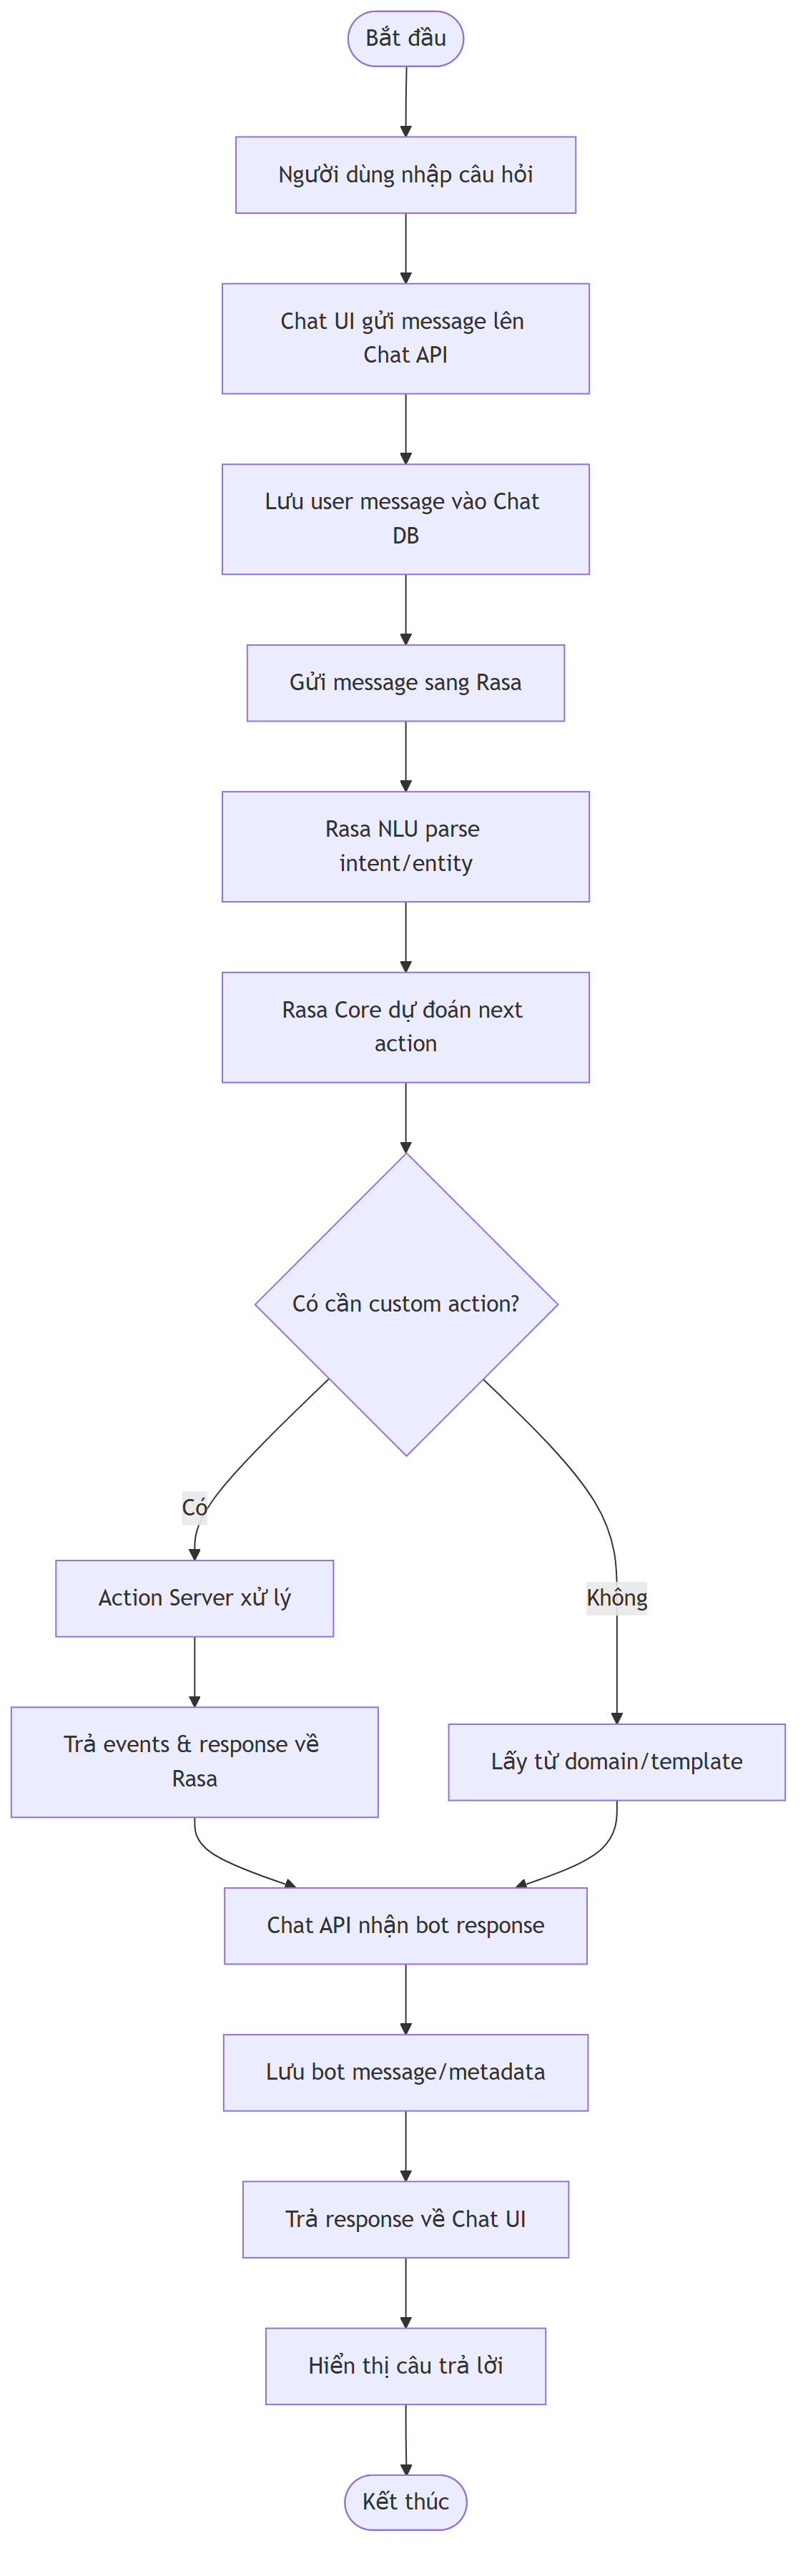
\includegraphics[width=\textwidth,height=0.78\textheight,keepaspectratio]{content/source/mermaid_activity/act_01.png}
    \caption{Activity Diagram luồng chat thường qua Rasa}
    \label{fig:act-chat-rasa}
\end{figure}



\section{Luồng xử lý câu hỏi bằng Rasa}

Rasa được dùng cho các câu hỏi có cấu trúc rõ ràng, có thể định nghĩa trước bằng intent, entity, rule và story.

Ví dụ câu hỏi:
\begin{itemize}
    \item Trường có những ngành nào?
    \item Ngành Công nghệ thông tin xét tuyển tổ hợp nào?
    \item Điểm chuẩn ngành An toàn thông tin năm 2024 là bao nhiêu?
\end{itemize}

Luồng xử lý bằng Rasa:
\begin{enumerate}
    \item Rasa nhận tin nhắn từ Backend API.
    \item NLU phân tích và xác định intent.
    \item Trích xuất entity (tên ngành, năm, phương thức xét tuyển...).
    \item Dialogue Management chọn hành động tiếp theo.
    \item Câu hỏi đơn giản: trả lời bằng template.
    \item Câu hỏi cần dữ liệu: gọi custom action.
    \item Action Server truy vấn Backend API/cơ sở dữ liệu.
    \item Kết quả trả về Rasa và gửi lại Backend API.
\end{enumerate}

Ưu điểm của luồng Rasa là tốc độ xử lý nhanh, dễ kiểm soát câu trả lời và phù hợp với câu hỏi lặp lại. Hạn chế là cần dữ liệu huấn luyện tương đối đầy đủ.

\begin{figure}[H]
    \centering
    \includegraphics[width=\textwidth,height=0.78\textheight,keepaspectratio]{content/source/mermaid_sequence/IMG/Luồng chat thường qua Rasa.png}
    \caption{Luồng xử lý câu hỏi bằng Rasa từ giao diện chat đến Action Server}
    \label{fig:seq-rasa-question-flow}
\end{figure}



\section{Luồng xử lý câu hỏi bằng RAG}

Luồng xử lý bằng RAG được sử dụng khi câu hỏi cần khai thác thông tin từ tài liệu tuyển sinh hoặc khi Rasa không đủ tự tin để trả lời.

Các trường hợp thường dùng RAG:
\begin{itemize}
    \item Câu hỏi dài, phức tạp.
    \item Câu hỏi cần tổng hợp nhiều nguồn.
    \item Câu hỏi liên quan quy chế/thông báo/đề án tuyển sinh.
    \item Câu hỏi chưa có trong tập intent.
    \item Câu hỏi cần trích dẫn nguồn.
\end{itemize}

\subsection*{a. Indexing Flow}

Indexing Flow là quá trình xử lý tài liệu đầu vào để tạo kho tri thức.
\begin{enumerate}
    \item Tải tài liệu tuyển sinh lên hệ thống.
    \item Lưu tài liệu gốc vào Document Store.
    \item Trích xuất, làm sạch và chuẩn hóa văn bản.
    \item Chia tài liệu thành các đoạn nhỏ và gắn metadata.
    \item Sinh embedding cho từng đoạn.
    \item Lưu embedding vào Vector Store.
    \item Trích xuất thực thể -- quan hệ quan trọng vào Knowledge Graph (nếu cần).
\end{enumerate}

\textbf{Gợi ý chèn Hình 3.5:} Indexing Flow của RAG.

\subsection*{b. Query Flow}

Query Flow là quá trình truy hồi và sinh câu trả lời khi người dùng đặt câu hỏi.
\begin{enumerate}
    \item Câu hỏi được chuyển từ Rasa/Action Server sang RAG.
    \item Chuẩn hóa câu hỏi và chuyển thành embedding.
    \item Vector Store tìm đoạn tài liệu liên quan.
    \item Document Store trả về nội dung đầy đủ.
    \item Có thể bổ sung ngữ cảnh bằng Knowledge Graph.
    \item Xếp hạng lại đoạn tài liệu, tạo prompt chứa câu hỏi + bằng chứng.
    \item Mô hình sinh ngôn ngữ tạo câu trả lời.
    \item Hệ thống gắn nguồn trích dẫn và trả về người dùng.
\end{enumerate}

\textbf{Gợi ý chèn Hình 3.6:} Query Flow của RAG.



\section{Thiết kế tích hợp Rasa, RAG và Backend API}

Việc tích hợp Rasa, RAG và Backend API là nội dung trọng tâm trong kiến trúc hệ thống. Thiết kế theo hướng phối hợp giúp khai thác thế mạnh từng thành phần thay vì thay thế lẫn nhau.

\subsection*{a. Nguyên tắc tích hợp}

\begin{itemize}
    \item Frontend chỉ giao tiếp với Backend API.
    \item Backend API chịu trách nhiệm xác thực, phân quyền và ghi log.
    \item Backend gửi tin nhắn đến Rasa để xử lý hội thoại.
    \item Action Server là cầu nối giữa Rasa, Backend API và RAG.
    \item RAG chỉ được gọi khi cần truy hồi tài liệu hoặc khi Rasa không đủ tự tin.
    \item Kết quả cuối cùng trả về Frontend thông qua Backend API.
\end{itemize}

\subsection*{b. Cơ chế lựa chọn giữa Rasa và RAG}

\begin{itemize}
    \item Câu hỏi ngắn, rõ intent: ưu tiên Rasa.
    \item Câu hỏi cần dữ liệu có cấu trúc: Rasa + Action Server + Backend API.
    \item Câu hỏi cần đọc tài liệu dài hoặc cần trích dẫn: RAG.
    \item Câu hỏi ngoài intent đã huấn luyện: fallback sang RAG.
\end{itemize}

Ví dụ:
\begin{itemize}
    \item ``Trường có những ngành nào?'' $\rightarrow$ Rasa $\rightarrow$ Action Server $\rightarrow$ Backend API $\rightarrow$ Database.
    \item ``Theo đề án tuyển sinh, điều kiện xét tuyển học bạ là gì?'' $\rightarrow$ Rasa fallback $\rightarrow$ Action Server $\rightarrow$ RAG.
\end{itemize}

\subsection*{c. Thiết kế API tích hợp}

Các API tiêu biểu:
\begin{itemize}
    \item \texttt{/api/chat/send} (POST): Gửi tin nhắn từ Frontend.
    \item \texttt{/api/chat/history} (GET): Lấy lịch sử hội thoại.
    \item \texttt{/api/admissions/majors} (GET): Lấy danh sách ngành.
    \item \texttt{/api/admissions/methods} (GET): Lấy phương thức xét tuyển.
    \item \texttt{/api/documents/upload} (POST): Tải tài liệu tuyển sinh.
    \item \texttt{/api/rag/index} (POST): Kích hoạt indexing tài liệu.
    \item \texttt{/api/rag/query} (POST): Truy vấn phân hệ RAG.
    \item \texttt{/api/admin/users} (GET/POST/PUT/DELETE): Quản lý người dùng.
    \item \texttt{/api/admin/logs} (GET): Xem log hệ thống.
\end{itemize}

\subsection*{d. Fallback từ Rasa sang RAG}

Cơ chế fallback giúp hệ thống không dừng ở phản hồi ``không hiểu'' khi intent có độ tin cậy thấp.

Quy trình:
\begin{enumerate}
    \item Rasa nhận câu hỏi và đánh giá confidence.
    \item Nếu confidence thấp, kích hoạt fallback action.
    \item Action Server gửi câu hỏi sang RAG.
    \item RAG truy hồi bằng chứng và sinh câu trả lời.
    \item Nếu không có bằng chứng phù hợp, hệ thống trả lời lịch sự và gợi ý người dùng hỏi rõ hơn.
\end{enumerate}

\begin{figure}[H]
    \centering
    \includegraphics[width=\textwidth,height=0.78\textheight,keepaspectratio]{content/source/mermaid_sequence/IMG/Luồng chat stream có phân nhánh Rasa RAG và fallback RAG.png}
    \caption{Sequence Diagram luồng chat stream có phân nhánh Rasa/RAG và fallback RAG}
    \label{fig:seq-stream-rasa-rag-fallback}
\end{figure}

\begin{figure}[H]
    \centering
    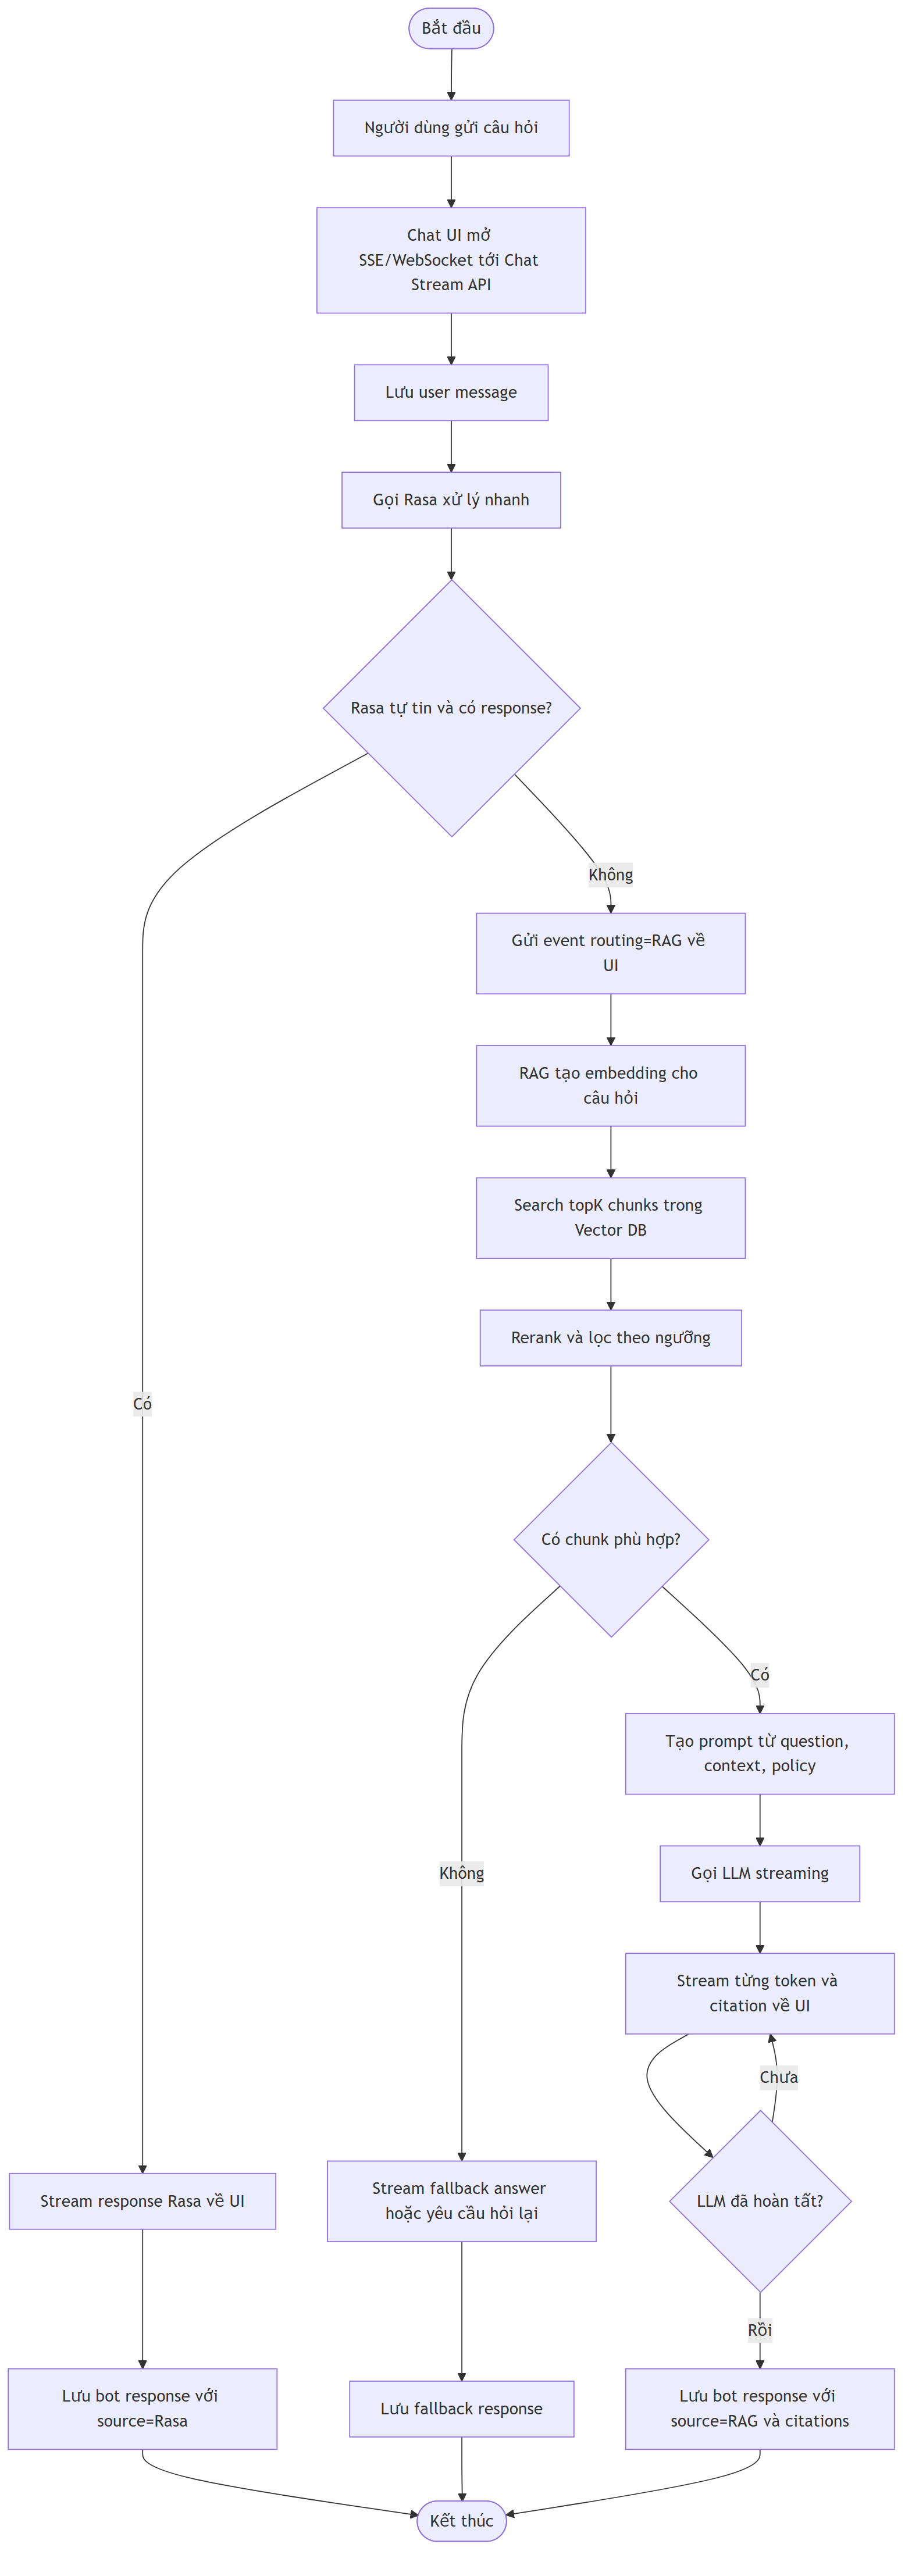
\includegraphics[width=\textwidth,height=0.78\textheight,keepaspectratio]{content/source/mermaid_activity/act_02.png}
    \caption{Activity Diagram luồng chat stream có phân nhánh Rasa/RAG và fallback RAG}
    \label{fig:act-stream-rasa-rag-fallback}
\end{figure}



\section{Thiết kế bảo mật và phân quyền tổng thể}

Bảo mật và phân quyền là yêu cầu quan trọng trong hệ thống trợ lý ảo tuyển sinh, đặc biệt khi hệ thống có phân hệ quản trị, dữ liệu người dùng và kho tài liệu RAG.

\subsection*{a. Xác thực người dùng}

Hệ thống có thể sử dụng JWT hoặc session-based authentication.

Yêu cầu chính:
\begin{itemize}
    \item Mật khẩu được băm an toàn, không lưu plaintext.
    \item Access token có thời hạn sử dụng.
    \item Có cơ chế đăng xuất và thu hồi phiên.
    \item API quản trị bắt buộc xác thực.
\end{itemize}

\subsection*{b. Phân quyền người dùng}

Các vai trò điển hình:
\begin{itemize}
    \item Guest: hỏi đáp tuyển sinh cơ bản.
    \item User: hỏi đáp và xem lịch sử hội thoại cá nhân.
    \item Admission Staff: quản lý dữ liệu tuyển sinh.
    \item Admin: quản lý toàn bộ hệ thống.
    \item Super Admin: quản lý tài khoản quản trị cấp cao và cấu hình hệ thống.
\end{itemize}

\subsection*{c. Bảo vệ API}

\begin{itemize}
    \item Kiểm tra token và kiểm tra vai trò trước khi truy cập API nhạy cảm.
    \item Validate dữ liệu đầu vào, giới hạn kích thước upload.
    \item Giới hạn tần suất request.
    \item Không trả lỗi chứa thông tin nhạy cảm.
    \item Sử dụng HTTPS khi triển khai thực tế.
\end{itemize}

\subsection*{d. Bảo mật dữ liệu RAG}

\begin{itemize}
    \item Chỉ quản trị viên có quyền tải lên/xóa tài liệu.
    \item Kiểm tra định dạng tài liệu trước xử lý.
    \item Không cho người dùng thường truy cập trực tiếp Document Store và Vector Store.
    \item Lưu metadata người tải, thời gian tải, trạng thái xử lý.
    \item Câu trả lời RAG phải dựa trên tài liệu đã kiểm duyệt.
\end{itemize}

\subsection*{e. Kiểm soát dữ liệu đầu vào}

\begin{itemize}
    \item Giới hạn độ dài câu hỏi và loại bỏ ký tự nguy hiểm.
    \item Kiểm tra nội dung trước khi gửi tới mô hình sinh.
    \item Ngăn prompt injection ở mức cơ bản.
    \item Từ chối yêu cầu tiết lộ thông tin hệ thống nội bộ.
\end{itemize}

\subsection*{f. Ghi log và giám sát}

Các nhóm log cần lưu:
\begin{itemize}
    \item Log đăng nhập.
    \item Log thao tác quản trị.
    \item Log upload/indexing tài liệu.
    \item Log câu hỏi và câu trả lời.
    \item Log lỗi khi gọi Rasa, Action Server, RAG.
    \item Log thời gian phản hồi.
\end{itemize}

\subsection*{g. Tổng kết thiết kế bảo mật}

Thiết kế bảo mật tổng thể dựa trên nguyên tắc: đúng quyền, đúng phạm vi truy cập, Backend API làm lớp kiểm soát trung tâm, dữ liệu nhạy cảm được bảo vệ, thao tác quan trọng được ghi log và hệ thống có cơ chế xử lý lỗi an toàn.





\chapter{PHÂN TÍCH VÀ THIẾT KẾ CHATBOT RASA CHO TƯ VẤN TUYỂN SINH}


\section{Vai trò của chatbot Rasa trong hệ thống}

Trong hệ thống KMA Chatbot tuyển sinh, Rasa đóng vai trò là phân hệ hội thoại chính dùng để xử lý các câu hỏi phổ biến, các luồng hỏi đáp định sẵn và các nghiệp vụ có cấu trúc rõ ràng. Khác với mô hình sinh văn bản tự do, Rasa được thiết kế theo hướng kiểm soát luồng hội thoại, trong đó mỗi câu hỏi của người dùng được phân tích thành ý định, trạng thái hội thoại và hành động phản hồi tương ứng.

Trước khi phân tích kiến trúc Rasa sử dụng NLU và PhoBERT, cần phân biệt với mô hình chatbot dựa trên luật. Chatbot rule-based vận hành chủ yếu dựa vào tập quy tắc if--then, từ khóa và các mẫu câu được định nghĩa trước. Cách tiếp cận này đơn giản, dễ kiểm soát nhưng kém linh hoạt khi người dùng diễn đạt câu hỏi theo nhiều cách khác nhau.

\begin{figure}[H]
    \centering
    \includegraphics[width=0.82\textwidth]{content/source/rasa/trợ lý ảo dựa trên rule.png}
    \caption{Kiến trúc chatbot dựa trên luật}
    \label{fig:rasa-rule-based-assistant}
\end{figure}

Hình~\ref{fig:rasa-rule-based-assistant} mô tả kiến trúc chatbot dựa trên luật. Câu hỏi của người dùng được đưa qua bộ xử lý ngôn ngữ để tách từ khóa, chuẩn hóa văn bản và so khớp với tập quy tắc. Nếu tìm được quy tắc phù hợp, hệ thống lấy câu trả lời từ cơ sở dữ liệu hoặc bộ tạo phản hồi. Ưu điểm của kiến trúc này là dễ triển khai và dễ kiểm soát nội dung. Tuy nhiên, khi câu hỏi có nhiều cách diễn đạt khác nhau hoặc chứa ngữ cảnh phức tạp, chatbot rule-based dễ thất bại do phụ thuộc mạnh vào từ khóa và luật được viết thủ công.

Khác với cách tiếp cận rule-based, Rasa kết hợp NLU, intent classification, entity extraction, tracker, policy và action để xử lý hội thoại linh hoạt hơn. Khi tích hợp PhoBERTIntentClassifier, hệ thống không chỉ so khớp từ khóa mà còn học biểu diễn ngữ nghĩa của câu hỏi tiếng Việt, từ đó phân biệt tốt hơn các intent gần nghĩa như hỏi điểm chuẩn, hỏi phương thức xét tuyển, hỏi học phí hoặc hỏi chương trình đào tạo.

\begin{figure}[H]
    \centering
    \includegraphics[width=0.9\textwidth]{content/source/rasa/trợ lý ảo dựa trên NLP.png}
    \caption{Kiến trúc trợ lý ảo dựa trên NLP và mô hình học máy}
    \label{fig:rasa-nlp-based-assistant}
\end{figure}

Hình~\ref{fig:rasa-nlp-based-assistant} thể hiện hướng tiếp cận chatbot dựa trên NLP và học máy. Câu hỏi của người dùng được phân tích để nhận diện ý định, trích xuất thông tin quan trọng và chuyển thành dữ liệu có cấu trúc cho bộ quản lý hội thoại.

Luồng chat thường của hệ thống bắt đầu từ giao diện hội thoại tại route \texttt{/} hoặc \texttt{/home\_chat}. Người dùng nhập câu hỏi vào giao diện, frontend gửi nội dung về backend chatbot, sau đó backend phối hợp với Rasa để xác định intent, entity, rule/story và action phù hợp. Phạm vi nghiệp vụ chính gồm tư vấn phương thức tuyển sinh, học phí, giấy báo trúng tuyển, hồ sơ nhập học và thông tin ngành đào tạo.

Trong kiến trúc tổng thể, Rasa không trực tiếp thay thế toàn bộ hệ thống hỏi đáp, mà đảm nhiệm phần hiểu ý định và điều phối hội thoại. Khi người dùng hỏi các câu thuộc nhóm đã được định nghĩa sẵn, Rasa có thể phản hồi nhanh bằng template trong domain. Khi câu hỏi cần xử lý logic hoặc không đủ chắc chắn, Rasa chuyển sang custom action hoặc fallback để tránh trả lời sai.

Vì vậy, phân hệ Rasa được thiết kế theo nguyên tắc: câu hỏi đơn giản và phổ biến được xử lý bằng intent, rule và response template; câu hỏi cần logic được xử lý bằng action server; câu hỏi mơ hồ hoặc ngoài phạm vi được đưa vào fallback hoặc ghi log để cải thiện dữ liệu huấn luyện.




\section{Kiến trúc thành phần của Rasa}

Rasa được tổ chức thành nhiều thành phần phối hợp với nhau để tạo thành một pipeline hội thoại hoàn chỉnh. Các thành phần quan trọng gồm Agent, NLU Pipeline, Dialogue Policies, Tracker Store, Lock Store, Domain, File System và Action Server.

\begin{figure}[H]
    \centering
    \includegraphics[width=0.95\textwidth]{content/source/rasa/các thành phần hệ thống rasa.png}
    \caption{Các thành phần chính trong kiến trúc Rasa}
    \label{fig:rasa-components}
\end{figure}

Hình~\ref{fig:rasa-components} cho thấy kiến trúc nội bộ của Rasa. Agent là thành phần điều phối trung tâm. NLU Pipeline chịu trách nhiệm phân tích câu hỏi để tạo intent, entity và confidence. Dialogue Policies sử dụng trạng thái hội thoại để chọn hành động tiếp theo. Tracker Store lưu lịch sử hội thoại và trạng thái slot. Lock Store giúp kiểm soát truy cập đồng thời khi nhiều message đến cùng một phiên. Domain định nghĩa phạm vi hoạt động của chatbot, bao gồm intents, entities, slots, responses và actions.

Action Server là thành phần mở rộng quan trọng. Khi Rasa Core chọn một custom action, Rasa gửi trạng thái hội thoại hiện tại sang Action Server. Action Server có thể đọc tracker, gọi backend, kiểm tra dữ liệu nghiệp vụ, ghi log hoặc tạo phản hồi động.

\begin{table}[H]
\centering
\begin{tabular}{|p{4cm}|p{8.5cm}|}
\hline
\textbf{Thành phần} & \textbf{Vai trò trong thiết kế} \\
\hline
NLU Pipeline & Chuyển câu hỏi tự nhiên thành intent, entity, confidence và ranking. \\
\hline
Dialogue Management & Dựa trên intent, slot và lịch sử để chọn action tiếp theo. \\
\hline
Tracker Store & Lưu trạng thái hội thoại, slot và lịch sử các hành động. \\
\hline
Domain & Định nghĩa intents, entities, slots, responses, forms và actions hợp lệ. \\
\hline
NLG Template & Sinh các phản hồi cố định, ổn định và dễ kiểm soát. \\
\hline
Action Server & Thực hiện logic nghiệp vụ, fallback nâng cao và ghi nhận câu hỏi chưa xử lý. \\
\hline
\end{tabular}
\caption{Vai trò các thành phần chính trong Rasa}
\label{tab:rasa-components-role}
\end{table}

Thiết kế này giúp chatbot không chỉ là một bộ phân loại intent. Rasa là một hệ thống hội thoại gồm nhiều lớp, trong đó NLU hiểu câu hỏi, Core chọn hành động, NLG sinh phản hồi, còn Tracker duy trì trạng thái để xử lý hội thoại nhiều lượt.




\section{Luồng tổng thể từ câu hỏi đến phản hồi}

Luồng xử lý tổng thể trong hệ thống được triển khai theo chuỗi gọi giữa frontend, backend và cụm Rasa. Từ hook \texttt{useChat} ở frontend, tin nhắn được gắn \texttt{conversationId} nếu chưa tồn tại, gửi tới endpoint \texttt{/api/v1/chatbot/\{id\}/chat}, sau đó backend chuyển tiếp sang Flask API và Rasa để lấy phản hồi.

\begin{figure}[H]
    \centering
    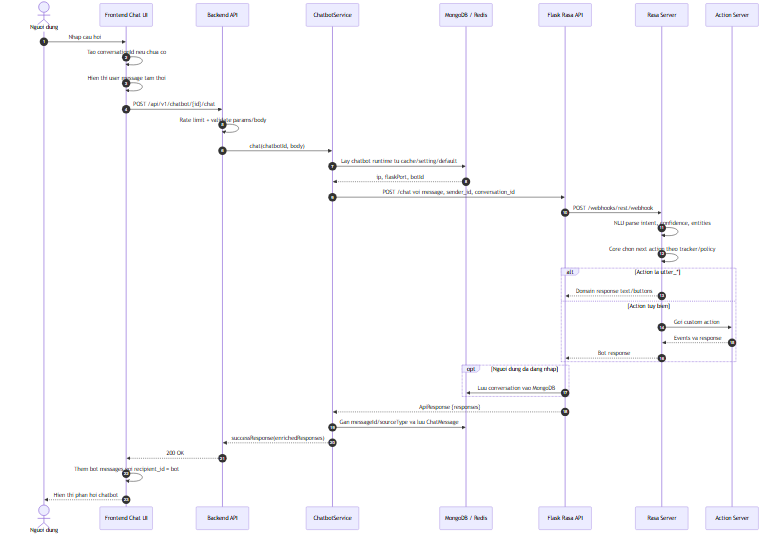
\includegraphics[width=\textwidth,height=0.82\textheight,keepaspectratio]{content/source/rasa/sequence/seq_2_2_3_question_to_answer.png}
    \caption{Sequence Diagram luồng tổng thể từ câu hỏi đến phản hồi chatbot}
    \label{fig:rasa-question-to-answer-flow}
\end{figure}

Trong sequence diagram này có thể thấy backend không chỉ đóng vai trò trung chuyển. Tầng service còn thực hiện chọn chatbot runtime, chuyển đổi dữ liệu sang định dạng Flask API cần dùng, đồng thời gắn \texttt{messageId}, \texttt{sourceType} và lưu phản hồi vào MongoDB để phục vụ lịch sử hội thoại và đánh giá chất lượng trả lời. Ở phía Flask, Rasa được gọi qua REST webhook; nếu cần custom action thì Action Server sẽ tham gia trước khi phản hồi cuối cùng quay lại frontend.



\section{Cấu trúc xử lý trong một lượt hội thoại}

Trong một lượt hội thoại, message của người dùng lần lượt đi qua các nhóm NLU, tracker, policy, NLG và custom action. Các khối này liên kết với nhau theo đúng thứ tự thực thi trong Rasa thay vì hoạt động độc lập.

\begin{figure}[H]
    \centering
    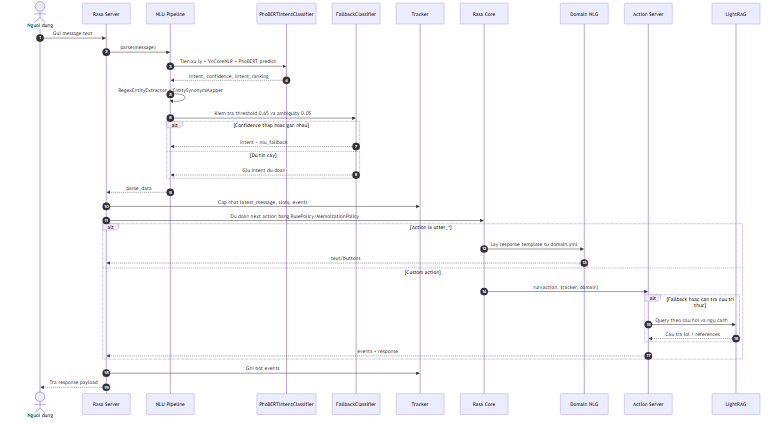
\includegraphics[width=\textwidth,height=0.82\textheight,keepaspectratio]{content/source/rasa/sequence/seq_2_2_4_dialogue_turn.png}
    \caption{Sequence Diagram cấu trúc xử lý trong một lượt hội thoại}
    \label{fig:rasa-dialogue-processing-groups}
\end{figure}

Hình~\ref{fig:rasa-dialogue-processing-groups} cho thấy các điểm quyết định quan trọng trong một lượt hội thoại. Sau khi \texttt{PhoBERTIntentClassifier} và các thành phần entity hoàn tất xử lý, \texttt{FallbackClassifier} kiểm tra confidence và độ nhập nhằng của intent. Nếu đạt ngưỡng, Rasa Core tiếp tục chọn action bằng \texttt{RulePolicy} và \texttt{MemoizationPolicy}; nếu không đạt, luồng sẽ chuyển sang nhánh fallback. Với các action dạng \texttt{utter\_*}, hệ thống lấy phản hồi từ \texttt{domain.yml}; còn với các action nghiệp vụ hoặc truy xuất tri thức, Action Server và LightRAG mới được gọi.



\section{Thiết kế tầng NLU cho tiếng Việt}

Tầng NLU là điểm vào đầu tiên của Rasa pipeline, có nhiệm vụ biến câu hỏi tiếng Việt thành dữ liệu có cấu trúc gồm intent, confidence, intent ranking và entity. Theo mã nguồn hiện tại, pipeline đang dùng \texttt{PhoBERTIntentClassifier}, \texttt{RegexEntityExtractor}, \texttt{EntitySynonymMapper} và \texttt{FallbackClassifier}.

\begin{figure}[H]
    \centering
    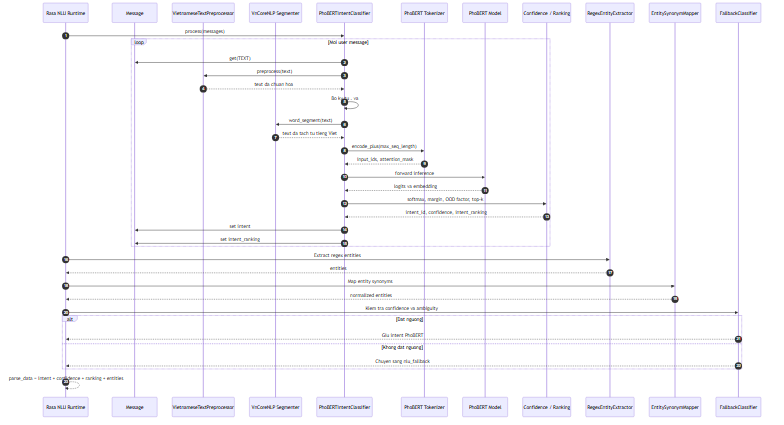
\includegraphics[width=\textwidth,height=0.82\textheight,keepaspectratio]{content/source/rasa/sequence/seq_2_2_5_nlu_pipeline.png}
    \caption{Sequence Diagram luồng xử lý NLU tiếng Việt với PhoBERT}
    \label{fig:rasa-nlu-sequence}
\end{figure}

Trong code, \texttt{PhoBERTIntentClassifier} thực hiện chuỗi xử lý gồm chuẩn hóa văn bản, loại bớt một số ký tự, tách từ bằng VnCoreNLP, token hóa bằng PhoBERT tokenizer, suy luận trên mô hình và tạo \texttt{intent\_ranking}. Sau đó \texttt{RegexEntityExtractor} và \texttt{EntitySynonymMapper} bổ sung, chuẩn hóa entity; cuối cùng \texttt{FallbackClassifier} kiểm tra ngưỡng \texttt{0.65} và độ nhập nhằng \texttt{0.05} để quyết định giữ intent hay chuyển sang \texttt{nlu\_fallback}. PhoBERT chỉ đảm nhiệm bước hiểu câu hỏi, còn việc chọn phản hồi vẫn do Rasa Core và Action Server quyết định.



\section{Thiết kế PhoBERTIntentClassifier}

PhoBERTIntentClassifier là thành phần quan trọng trong thiết kế NLU tiếng Việt. Thành phần này nhận câu hỏi đã được chuẩn hóa và tách từ, sau đó sử dụng PhoBERT để tạo biểu diễn ngữ nghĩa toàn câu. Biểu diễn này được đưa qua lớp phân loại để dự đoán intent và confidence.

\begin{figure}[H]
    \centering
    \includegraphics[width=0.98\textwidth]{content/source/rasa/Cấu trúc module NLU và PhoBERTIntentClassifier.png}
    \caption{Cấu trúc module NLU và PhoBERTIntentClassifier}
    \label{fig:rasa-nlu-phobert-classifier}
\end{figure}

Hình~\ref{fig:rasa-nlu-phobert-classifier} thể hiện đầy đủ các bước chính: preprocessor, VnCoreNLP, tokenizer, tensor input, PhoBERT encoder, pooling, classification head, softmax, ranking, confidence calibration và fallback gate. Đây là cấu trúc giúp Rasa hiểu câu hỏi ở mức ngữ nghĩa thay vì chỉ khớp từ khóa.

\begin{figure}[H]
    \centering
    \includegraphics[width=0.98\textwidth]{content/source/rasa/Kiến trúc xử lý của PhoBERT trong bài toán phân loại intent.png}
    \caption{Kiến trúc xử lý của PhoBERT trong bài toán phân loại intent tiếng Việt}
    \label{fig:rasa-phobert-intent-architecture}
\end{figure}

Hình~\ref{fig:rasa-phobert-intent-architecture} đi sâu hơn vào cơ chế PhoBERT cho intent classification. Sau khi được token hóa, câu hỏi được đưa qua PhoBERT encoder để tạo vector ngữ cảnh. Vector này đi qua pooling và classification head, sau đó softmax tính xác suất cho từng intent. Intent có xác suất cao nhất được đề xuất cho Dialogue Management, miễn là vượt qua ngưỡng confidence.

Để làm rõ hơn vai trò của PhoBERTIntentClassifier, có thể xét một ví dụ cụ thể. Câu hỏi ban đầu của người dùng được chuẩn hóa, tách từ, mã hóa thành embedding, đưa qua tầng softmax để tính xác suất intent và cuối cùng trả về output cho Rasa gồm intent, confidence và ranking.

\begin{figure}[H]
    \centering
    \includegraphics[width=0.98\textwidth]{content/source/rasa/Ví dụ biến đổi câu hỏi qua PhoBERTIntentClassifier .png}
    \caption{Ví dụ biến đổi câu hỏi qua PhoBERTIntentClassifier}
    \label{fig:rasa-phobert-question-transform}
\end{figure}

Hình~\ref{fig:rasa-phobert-question-transform} minh họa quá trình biến đổi một câu hỏi tiếng Việt qua PhoBERTIntentClassifier. Câu hỏi gốc trước hết được chuẩn hóa để giảm nhiễu ký tự và thống nhất chữ viết. Sau đó, văn bản được tách từ để tạo chuỗi token phù hợp với tiếng Việt. PhoBERT tiếp tục mã hóa chuỗi token thành biểu diễn ngữ nghĩa toàn câu. Tầng softmax tính xác suất cho từng intent, ví dụ intent hỏi điểm chuẩn đạt xác suất cao nhất. Kết quả cuối cùng được trả về cho Rasa dưới dạng intent, confidence và intent ranking để Dialogue Management lựa chọn action tiếp theo.




\section{Thiết kế intent, entity và dữ liệu huấn luyện}

Intent là nhãn biểu diễn mục đích của người dùng. Trong hệ thống tư vấn tuyển sinh, intent cần được thiết kế theo nhóm nghiệp vụ thay vì thiết kế rời rạc theo từng câu hỏi cụ thể.

\begin{table}[H]
\centering
\begin{tabular}{|p{4cm}|p{8.5cm}|}
\hline
\textbf{Nhóm intent} & \textbf{Intent tiêu biểu} \\
\hline
Giao tiếp cơ bản & \texttt{chao\_hoi}, \texttt{cam\_on}, \texttt{tam\_biet}, \texttt{hoi\_kha\_nang\_ho\_tro} \\
\hline
Tuyển sinh & \texttt{hoi\_phuong\_thuc\_tuyen\_sinh}, \texttt{hoi\_to\_hop\_xet\_tuyen}, \texttt{hoi\_diem\_chuan}, \texttt{hoi\_chi\_tieu\_tuyen\_sinh}, \texttt{hoi\_thoi\_gian\_tuyen\_sinh}, \texttt{hoi\_dieu\_kien\_xet\_tuyen} \\
\hline
Ngành đào tạo & \texttt{hoi\_nganh\_an\_toan\_thong\_tin}, \texttt{hoi\_nganh\_cong\_nghe\_thong\_tin}, \texttt{hoi\_nganh\_dien\_tu\_vien\_thong}, \texttt{hoi\_chuong\_trinh\_dao\_tao}, \texttt{hoi\_co\_hoi\_viec\_lam} \\
\hline
Thủ tục & \texttt{hoi\_ho\_so\_nhap\_hoc}, \texttt{hoi\_giay\_bao\_trung\_tuyen}, \texttt{hoi\_hoc\_phi}, \texttt{hoi\_ky\_tuc\_xa}, \texttt{hoi\_bao\_hiem\_y\_te} \\
\hline
Điều khiển hội thoại & \texttt{yeu\_cau\_tom\_tat}, \texttt{yeu\_cau\_noi\_ro\_hon}, \texttt{hoi\_nguon\_thong\_tin}, \texttt{nlu\_fallback} \\
\hline
\end{tabular}
\caption{Các nhóm intent chính trong chatbot tuyển sinh}
\label{tab:rasa-intent-groups}
\end{table}

Entity là thông tin cụ thể cần trích xuất trong câu hỏi. Với hệ thống tuyển sinh, entity có thể gồm \texttt{nganh}, \texttt{ma\_nganh}, \texttt{to\_hop\_mon}, \texttt{nam\_tuyen\_sinh}, \texttt{phuong\_thuc\_xet\_tuyen}, \texttt{co\_so\_dao\_tao}, \texttt{loai\_giay\_to} và \texttt{doi\_tuong\_thi\_sinh}.

Ví dụ, với câu hỏi ``Ngành An toàn thông tin năm 2025 lấy bao nhiêu điểm?'', hệ thống cần nhận diện intent là \texttt{hoi\_diem\_chuan}, entity \texttt{nganh} là ``An toàn thông tin'' và entity \texttt{nam\_tuyen\_sinh} là ``2025''.

Dữ liệu huấn luyện cần có nhiều biến thể cho mỗi intent để mô hình học được ý định thay vì học thuộc một câu cụ thể. Ví dụ với intent \texttt{hoi\_hoc\_phi}, dữ liệu mẫu có thể gồm: ``học phí của học viện là bao nhiêu'', ``ngành công nghệ thông tin học phí thế nào'', ``em muốn hỏi mức học phí năm nay'', ``học phí một kỳ khoảng bao nhiêu'', ``học phí ngành an toàn thông tin có cao không''.

Việc thiết kế intent và entity phải bảo đảm ba yêu cầu: đủ bao phủ nghiệp vụ tuyển sinh, không trùng nghĩa quá gần giữa các intent, và có dữ liệu mẫu đa dạng theo cách hỏi thực tế của người dùng.




\section{Thiết kế Dialogue Management}

Dialogue Management là lớp quyết định chatbot sẽ làm gì sau khi NLU đã phân tích câu hỏi. Đây là phần biến intent thành action.

Công thức khái quát có thể mô tả như sau:

\[
action_t = Policy(intent_t, confidence_t, entity_t, slots_t, history_t)
\]

Trong đó, \texttt{intent\_t} là ý định hiện tại của người dùng, \texttt{confidence\_t} là độ tin cậy của intent, \texttt{entity\_t} là thực thể được trích xuất, \texttt{slots\_t} là trạng thái hội thoại đang lưu và \texttt{history\_t} là lịch sử các lượt hội thoại trước.

Rasa sử dụng các thành phần như RulePolicy, MemoizationPolicy hoặc TEDPolicy để quyết định action. Với các luồng đơn giản, RulePolicy được dùng để ánh xạ trực tiếp intent sang action, ví dụ \texttt{chao\_hoi} sang \texttt{utter\_chao\_hoi}, \texttt{cam\_on} sang \texttt{utter\_cam\_on}, \texttt{tam\_biet} sang \texttt{utter\_tam\_biet}.

\begin{figure}[H]
    \centering
    \includegraphics[width=0.95\textwidth]{content/source/rasa/Quan hệ giữa DM, domain, NLG template và action server.png}
    \caption{Quan hệ giữa Dialogue Manager, domain, NLG template và action server}
    \label{fig:rasa-dm-domain-nlg-action}
\end{figure}

Hình~\ref{fig:rasa-dm-domain-nlg-action} thể hiện mối quan hệ giữa intent ranking, tracker history, slot state, Dialogue Manager, template response và custom action. Nếu action được chọn là template, hệ thống lấy phản hồi từ domain. Nếu action cần xử lý nghiệp vụ, Rasa gọi Action Server.

Với các luồng cần ngữ cảnh, tracker và slot được sử dụng để ghi nhớ thông tin. Ví dụ, người dùng hỏi ``Ngành An toàn thông tin xét tổ hợp nào?'' rồi hỏi tiếp ``Thế điểm chuẩn năm ngoái là bao nhiêu?''. Ở lượt thứ hai, câu hỏi không nhắc lại tên ngành, nhưng hệ thống có thể dùng slot \texttt{nganh = An toàn thông tin} từ lượt trước để hiểu ngữ cảnh.

Thiết kế Dialogue Management cần bảo đảm chatbot xử lý được ba nhóm luồng: luồng một lượt, luồng nhiều lượt và luồng fallback. Luồng một lượt xảy ra khi người dùng hỏi rõ và hệ thống trả lời ngay. Luồng nhiều lượt xảy ra khi người dùng hỏi thiếu thông tin, bot hỏi lại và người dùng bổ sung. Luồng fallback xảy ra khi câu hỏi mơ hồ hoặc ngoài phạm vi, bot xin làm rõ hoặc ghi nhận câu hỏi.




\section{Thiết kế domain, NLG template và custom action}

Trong Rasa, \texttt{domain.yml} là nơi định nghĩa các thành phần chính của chatbot như intents, entities, slots, responses, actions và forms. Đối với hệ thống tư vấn tuyển sinh, domain đóng vai trò như bản thiết kế hành vi hội thoại.

Cấu trúc domain cần bao gồm các nhóm chính:

\begin{table}[H]
\centering
\begin{tabular}{|p{3.5cm}|p{9cm}|}
\hline
\textbf{Nhóm} & \textbf{Ví dụ thành phần} \\
\hline
Intents & \texttt{chao\_hoi}, \texttt{hoi\_hoc\_phi}, \texttt{hoi\_diem\_chuan}, \texttt{hoi\_to\_hop\_xet\_tuyen}, \texttt{hoi\_ho\_so\_nhap\_hoc}, \texttt{nlu\_fallback} \\
\hline
Entities & \texttt{nganh}, \texttt{nam\_tuyen\_sinh}, \texttt{to\_hop\_mon}, \texttt{phuong\_thuc\_xet\_tuyen} \\
\hline
Slots & \texttt{nganh}, \texttt{nam\_tuyen\_sinh}, \texttt{clarification\_count}, \texttt{pending\_question} \\
\hline
Responses & \texttt{utter\_chao\_hoi}, \texttt{utter\_hoc\_phi}, \texttt{utter\_diem\_chuan}, \texttt{utter\_hoi\_lam\_ro}, \texttt{utter\_fallback} \\
\hline
Actions & \texttt{action\_fallback}, \texttt{action\_log\_unknown\_question} \\
\hline
\end{tabular}
\caption{Cấu trúc thiết kế domain của chatbot Rasa}
\label{tab:rasa-domain-design}
\end{table}

NLG trong hệ thống Rasa chủ yếu là template-based. Điều này phù hợp với chatbot tuyển sinh vì nhiều câu trả lời cần ổn định, nhất quán và không được tự ý sinh thông tin sai. Ví dụ, phản hồi chào hỏi nên giới thiệu rõ vai trò chatbot và gợi ý các nhóm thông tin có thể hỗ trợ như ngành học, điểm chuẩn, học phí hoặc hồ sơ nhập học.

Ưu điểm của template là dễ kiểm soát nội dung. Nhược điểm là độ linh hoạt thấp nếu người dùng hỏi nhiều biến thể phức tạp. Vì vậy, template nên dùng cho các nhóm câu hỏi chắc chắn, còn các trường hợp cần xử lý điều kiện nên chuyển sang custom action.

Custom action là lớp xử lý nghiệp vụ khi response tĩnh trong domain không đủ. Khi Rasa Core chọn custom action, Rasa gửi tracker, domain và trạng thái hội thoại hiện tại sang Action Server để xử lý. Action Server đọc intent, entity, slot, lịch sử hội thoại, sau đó trả message qua dispatcher và event cập nhật tracker nếu cần.

Ba đối tượng quan trọng trong custom action gồm:

\begin{itemize}
    \item \texttt{dispatcher}: gửi message, button hoặc response về người dùng.
    \item \texttt{tracker}: đọc lịch sử hội thoại, intent, entity và slot.
    \item \texttt{domain}: chứa cấu hình hợp lệ của chatbot.
\end{itemize}

Ví dụ, \texttt{action\_fallback} có thể đọc intent ranking, \texttt{clarification\_count} và \texttt{pending\_question} để quyết định bot nên hỏi lại, gợi ý người dùng nhập rõ hơn hay ghi log câu hỏi chưa xử lý được.




\section{Thiết kế fallback và kiểm soát confidence}

Fallback là cơ chế bắt buộc trong chatbot tuyển sinh vì hệ thống không được trả lời tùy tiện khi không hiểu câu hỏi. FallbackClassifier kiểm tra confidence của intent. Nếu confidence thấp hơn ngưỡng thiết kế, hệ thống không chấp nhận intent mà chuyển sang nhánh fallback.

Logic xử lý có thể mô tả như sau:

\begin{center}
\begin{tabular}{c}
\texttt{Nếu max(confidence) >= threshold} \\
$\downarrow$ \\
\texttt{Chấp nhận intent} \\
\texttt{Ngược lại} \\
$\downarrow$ \\
\texttt{Kích hoạt fallback}
\end{tabular}
\end{center}

Fallback có thể chia thành nhiều cấp. Fallback cấp 1 là bot hỏi lại để làm rõ ý định. Fallback cấp 2 là bot gợi ý một số nhóm câu hỏi có thể hỗ trợ. Fallback cấp 3 là bot ghi log câu hỏi chưa xử lý được để quản trị viên bổ sung dữ liệu. Fallback cấp 4 là bot thông báo chưa có thông tin phù hợp thay vì tự trả lời.

Ví dụ, khi người dùng hỏi ``Cái ngành đó thì sao?'', bot có thể phản hồi: ``Bạn đang muốn hỏi về ngành nào ạ? Bạn có thể nhập tên ngành như An toàn thông tin, Công nghệ thông tin hoặc Điện tử viễn thông.''

Fallback không chỉ là xử lý lỗi. Đây là cơ chế bảo vệ chất lượng thông tin. Đặc biệt với lĩnh vực tuyển sinh, câu trả lời sai về điểm chuẩn, học phí, hồ sơ hoặc thời gian nhập học có thể gây ảnh hưởng trực tiếp đến người dùng. Vì vậy, khi không đủ chắc chắn, hệ thống nên hỏi lại hoặc từ chối có kiểm soát.

\subsection*{Thiết kế luồng hội thoại mẫu}

\subsection*{Luồng chào hỏi}

Luồng chào hỏi gồm bốn bước: người dùng nhập ``Xin chào'', NLU nhận diện intent \texttt{chao\_hoi}, Core chọn action \texttt{utter\_chao\_hoi}, sau đó bot phản hồi rằng hệ thống có thể hỗ trợ thông tin tuyển sinh, ngành học, học phí và hồ sơ nhập học.

Đây là luồng đơn giản, nên xử lý bằng rule và response template.

\subsection*{Luồng hỏi học phí}

Khi người dùng hỏi ``Học phí ngành An toàn thông tin là bao nhiêu?'', NLU cần nhận diện intent \texttt{hoi\_hoc\_phi} và entity \texttt{nganh = An toàn thông tin}. Core lưu slot ngành và chọn action trả lời học phí. Luồng này có thể dùng template nếu học phí cố định, hoặc custom action nếu học phí phụ thuộc ngành, năm học hoặc hệ đào tạo.

\subsection*{Luồng hỏi thiếu thông tin}

Khi người dùng hỏi ``Điểm chuẩn là bao nhiêu?'', hệ thống có thể nhận diện intent \texttt{hoi\_diem\_chuan} nhưng thiếu ngành và năm. Core kiểm tra slot bắt buộc và yêu cầu người dùng bổ sung: ``Bạn muốn hỏi điểm chuẩn ngành nào và năm nào?''. Sau khi người dùng trả lời ``Ngành Công nghệ thông tin năm 2025'', hệ thống cập nhật slot và trả lời theo thông tin phù hợp.

\subsection*{Luồng fallback}

Khi người dùng hỏi ``Cái kia đăng ký sao?'', confidence thấp hoặc intent không rõ. FallbackClassifier kích hoạt \texttt{nlu\_fallback}. Core chọn \texttt{action\_fallback}. Action đọc intent ranking, pending question và số lần hỏi lại, sau đó phản hồi: ``Bạn có thể nói rõ bạn muốn đăng ký nội dung nào không: xét tuyển, nhập học, ký túc xá hay giấy tờ?''



\section{Quy trình chuẩn bị dữ liệu và huấn luyện mô hình}

Quy trình huấn luyện trong hệ thống hiện tại gồm ba lớp công việc liên tiếp: chuẩn bị dữ liệu nghiệp vụ thành bộ file Rasa, huấn luyện \texttt{PhoBERTIntentClassifier} với cơ chế tự tối ưu tham số, và điều phối train ở mức hệ thống để sinh model mới rồi nạp lại vào chatbot. Vì vậy ba hình trong mục này cần phản ánh đúng luồng code thay vì tách riêng thành ``train intent'' và ``train NER'' như mô hình tổng quát thông thường.

\begin{figure}[H]
    \centering
    \includegraphics[width=\textwidth,height=0.8\textheight,keepaspectratio]{content/source/rasa/training/train_2_2_11_data_prep.png}
    \caption{Quy trình chuẩn bị dữ liệu huấn luyện cho Rasa PhoBERT}
    \label{fig:rasa-phobert-data-process}
\end{figure}

Hình~\ref{fig:rasa-phobert-data-process} mô tả lớp chuẩn bị dữ liệu. Ở đầu vào, dữ liệu đến từ FAQ, đề án tuyển sinh, kịch bản tư vấn và lịch sử hội thoại đã được chắt lọc. Backend tổng hợp các nội dung này thành \texttt{nlu.yml}, \texttt{stories.yml}, \texttt{rules.yml} và \texttt{domain.yml}, sau đó gửi sang Flask API qua \texttt{POST /train}. Trong \texttt{PhoBERTIntentClassifier}, từng câu hỏi tiếp tục được chuẩn hóa, loại bớt một số ký tự, tách từ bằng VnCoreNLP và ánh xạ sang \texttt{intent\_id}. Nếu đang ở chế độ fresh training và dữ liệu còn ít, bộ tăng cường dữ liệu sẽ tạo thêm paraphrase có kiểm soát để mở rộng biên phân loại.

Điểm quan trọng là hệ thống không huấn luyện một NER model độc lập trong luồng hiện tại. Entity chủ yếu được xử lý bằng \texttt{RegexEntityExtractor} và \texttt{EntitySynonymMapper}, còn trọng tâm của quá trình train là intent classification với PhoBERT. Vì vậy đầu ra của bước chuẩn bị dữ liệu là một tập huấn luyện intent đã được segment đúng tiếng Việt và lưu lại để dùng cho EWC ở các lần fine-tune sau.

\begin{figure}[H]
    \centering
    \includegraphics[width=\textwidth,height=0.82\textheight,keepaspectratio]{content/source/rasa/training/train_2_2_11_phobert_train.png}
    \caption{Quy trình huấn luyện PhoBERTIntentClassifier trong code hiện tại}
    \label{fig:rasa-train-intent}
\end{figure}

Hình~\ref{fig:rasa-train-intent} thể hiện lõi huấn luyện của \texttt{PhoBERTIntentClassifier}. Trước khi chạy vòng lặp train, \texttt{AutoParameterTuner} phân tích số lượng mẫu, số lớp intent, mức mất cân bằng, độ dài trung bình của câu và tình trạng fine-tune để tự chọn batch size, số epoch, learning rate, max sequence length, warmup ratio và nhiều tham số regularization khác. Nếu phát hiện đã tồn tại model cũ trong ModelStorage hoặc trong file \texttt{models/*.tar.gz}, hệ thống chuyển sang fine-tuning, bật adapter và EWC để giữ tri thức cũ; nếu không có model trước đó thì tạo mới toàn bộ \texttt{EnhancedPhoBERTClassifier}.

Bên trong vòng train, dữ liệu được chia train/validation theo stratified split để mỗi intent đều xuất hiện ở cả hai tập. Nếu bật contrastive learning, dataloader dùng \texttt{ClassBalancedBatchSampler} để mỗi batch có đủ positive pair cùng lớp. Hàm mất mát cuối cùng là tổ hợp của loss phân loại, contrastive loss và EWC loss; đồng thời code còn dùng FP16, gradient accumulation, gradient clipping, learning-rate scheduler có warmup và cơ chế tự giảm batch size khi GPU bị hết VRAM. Sau mỗi epoch, model được đo \texttt{val\_accuracy}, lưu best checkpoint và dừng sớm nếu không còn cải thiện. Kết thúc train, mô hình tốt nhất được phục hồi, sau đó tiếp tục hiệu chỉnh confidence bằng temperature scaling và tính class centroids để hỗ trợ phát hiện out-of-domain ở giai đoạn suy luận.

\begin{figure}[H]
    \centering
    \includegraphics[width=\textwidth,height=0.8\textheight,keepaspectratio]{content/source/rasa/training/train_2_2_11_train_orchestration.png}
    \caption{Quy trình điều phối train, đóng gói và kích hoạt model mới}
    \label{fig:rasa-train-ner}
\end{figure}

Hình cuối cùng mô tả quy trình điều phối train ở mức hệ thống. Khi backend hoặc admin gửi \texttt{POST /train}, Flask API kiểm tra xem đã có phiên train nào đang chạy hay chưa, ghi các file YAML mới ra đĩa, cập nhật lại \texttt{actions.py} nếu có custom action mới rồi khởi động lệnh \texttt{python -m rasa train} ở background thread. Nếu yêu cầu bật \texttt{firetune}, lệnh train sẽ thêm \texttt{--epoch-fraction 0.5} để rút ngắn thời gian hội tụ vì \texttt{PhoBERTIntentClassifier} đã tự nhận biết model cũ và chuyển sang fine-tune.

Sau khi lệnh train hoàn tất, hệ thống tìm file model \texttt{.tar.gz} trong thư mục \texttt{models/}, upload model đó lên MinIO, cập nhật thông tin model vào MongoDB và trả trạng thái qua API \texttt{/training-status}. Backend sau đó có thể poll trạng thái này và gọi tiếp \texttt{POST /run-model} để nạp model mới vào Rasa runtime. Cách tổ chức này cho phép tách riêng ba pha: chuẩn bị dữ liệu, huấn luyện mô hình và triển khai model sau huấn luyện, từ đó giúp quản trị viên kiểm soát rõ hơn quá trình cập nhật chatbot.



\section{Kiểm thử và đánh giá phân hệ Rasa}

Kiểm thử phân hệ Rasa cần tách thành nhiều lớp thay vì chỉ kiểm tra câu trả lời cuối cùng. Mỗi lớp kiểm thử giúp phát hiện một nhóm lỗi khác nhau trong quá trình vận hành chatbot.

Thứ nhất là kiểm thử NLU. Mục tiêu là đánh giá mô hình có nhận đúng intent và entity hay không. Các chỉ số có thể dùng gồm accuracy, precision, recall, F1-score, top-k accuracy và confusion matrix.

Thứ hai là kiểm thử rule/story. Mục tiêu là xác định khi NLU đúng thì Core có chọn đúng action hay không. Ví dụ, intent \texttt{hoi\_hoc\_phi} phải dẫn đến action trả lời học phí, không được dẫn sang action hỏi điểm chuẩn.

Thứ ba là kiểm thử fallback. Cần kiểm tra các câu hỏi mơ hồ, câu ngoài phạm vi, câu thiếu thông tin và câu có confidence thấp. Kết quả mong đợi là bot hỏi lại hoặc ghi log, không trả lời bừa.

Thứ tư là kiểm thử custom action. Cần kiểm tra action có đọc đúng slot, trả đúng message và cập nhật đúng event hay không.

\begin{table}[H]
\centering
\begin{tabular}{|p{3.5cm}|p{4.5cm}|p{5cm}|}
\hline
\textbf{Nhóm kiểm thử} & \textbf{Kịch bản} & \textbf{Kết quả mong đợi} \\
\hline
NLU & Hỏi học phí, điểm chuẩn, phương thức tuyển sinh & Nhận đúng intent và entity \\
\hline
Dialogue Management & Intent đúng nhưng cần chọn action phù hợp & Core chọn đúng utterance hoặc custom action \\
\hline
Slot & Người dùng hỏi thiếu ngành hoặc thiếu năm & Bot hỏi bổ sung thông tin \\
\hline
Fallback & Câu hỏi mơ hồ hoặc ngoài phạm vi & Bot hỏi lại hoặc ghi log \\
\hline
Custom Action & Gọi action fallback hoặc ghi log câu hỏi lỗi & Action trả đúng message và cập nhật đúng event \\
\hline
\end{tabular}
\caption{Bảng kiểm thử đề xuất cho phân hệ Rasa}
\label{tab:rasa-testing-plan}
\end{table}

Ngoài kiểm thử kỹ thuật, cần đánh giá theo góc nhìn nghiệp vụ tuyển sinh. Các câu trả lời về điểm chuẩn, học phí, hồ sơ, thời gian và điều kiện xét tuyển phải chính xác, nhất quán và không gây hiểu nhầm cho người dùng.



\section{Kết luận chương}

Chương này đã phân tích và thiết kế phân hệ chatbot Rasa theo hướng luồng hệ thống. Rasa được đặt ở vai trò điều phối hội thoại cho các câu hỏi tuyển sinh phổ biến, có cấu trúc và có thể kiểm soát bằng intent, entity, rule, story, domain response và custom action.

Luồng xử lý chính bắt đầu từ câu hỏi của người dùng, đi qua frontend, backend, Rasa Server, NLU pipeline, Dialogue Management, Action Selection và cuối cùng trả response về giao diện. Trong đó, NLU sử dụng xử lý tiếng Việt với VnCoreNLP và PhoBERT Intent Classifier để dự đoán intent; Core dùng tracker, slot và policy để chọn action; domain và action server tạo phản hồi cuối cùng.

Điểm quan trọng trong thiết kế là hệ thống không nên trả lời mọi câu hỏi bằng một nhánh duy nhất. Câu hỏi rõ ràng được trả lời trực tiếp bằng template hoặc action. Câu hỏi thiếu thông tin cần hỏi lại. Câu hỏi confidence thấp phải đi vào fallback. Câu hỏi chưa xử lý được cần ghi log để cải thiện dữ liệu huấn luyện. Cách thiết kế này giúp chatbot Rasa vận hành ổn định, dễ kiểm soát và phù hợp với yêu cầu tư vấn tuyển sinh.






\chapter{PHÂN TÍCH VÀ THIẾT KẾ PHÂN HỆ RAG}

\section{Vai trò của RAG trong hệ thống tư vấn tuyển sinh}

Phân hệ RAG, viết tắt của Retrieval-Augmented Generation, là thành phần chịu trách nhiệm xử lý các câu hỏi cần tri thức từ tài liệu tuyển sinh, chương trình đào tạo, điểm chuẩn, quy chế, biểu mẫu và các văn bản liên quan của Học viện. Khác với Rasa, vốn phù hợp với các intent định sẵn và các luồng hội thoại có cấu trúc, RAG được dùng khi câu trả lời cần dựa trên kho tài liệu đã được ingest, chunking và lập chỉ mục.

Trong hệ thống KMA Chatbot, RAG không được thiết kế như một mô hình tự trả lời theo trí nhớ của LLM. Thay vào đó, RAG hoạt động theo nguyên tắc: trước khi sinh câu trả lời, hệ thống phải truy hồi bằng chứng từ kho tài liệu, xây dựng ngữ cảnh, sau đó mới gọi LLM để diễn đạt câu trả lời. Cách thiết kế này giúp giảm nguy cơ hallucination, tăng khả năng truy vết nguồn và phù hợp với bài toán tuyển sinh, nơi thông tin như phương thức xét tuyển, điểm chuẩn, học phí hoặc chương trình đào tạo có thể thay đổi theo từng năm.

RAG không để LLM tự trả lời theo tri thức đã học sẵn, mà trước hết truy xuất thông tin liên quan từ kho tài liệu, sau đó đưa các bằng chứng này vào mô hình sinh để tạo câu trả lời có căn cứ.

\begin{figure}[H]
    \centering
    \includegraphics[width=0.9\textwidth]{content/source/RAG/mô hình RAG.png}
    \caption{Kiến trúc tổng quan của mô hình RAG}
    \label{fig:rag-basic-model}
\end{figure}

Trong dữ liệu kỹ thuật đã khảo sát, hệ thống có frontend web, backend API, RAG service ở port 9621 và các lớp lưu trữ phía sau. RAG service phụ trách ingest, chunking, indexing, retrieval và sinh câu trả lời theo tài liệu. Health endpoint cho thấy phân hệ RAG sử dụng embedding model BAAI/bge-m3, RedisKVStorage, RedisDocStatusStorage, MemgraphStorage và QdrantVectorDBStorage. Điều này cho thấy hệ thống đã được thiết kế theo hướng tách riêng metadata, trạng thái tài liệu, vector và đồ thị tri thức.

Về mặt chức năng, RAG đảm nhiệm các nhóm nhiệm vụ chính sau:

\begin{itemize}
    \item Tiếp nhận và xử lý tài liệu tuyển sinh, đào tạo, điểm chuẩn, biểu mẫu.
    \item Chia tài liệu thành các chunk có thể truy hồi.
    \item Sinh embedding cho chunk, entity và relation.
    \item Lưu trữ vector vào vector database.
    \item Lưu trạng thái xử lý tài liệu để quản trị viên theo dõi.
    \item Truy hồi bằng chứng khi người dùng đặt câu hỏi.
    \item Xây dựng context và gọi LLM sinh câu trả lời.
    \item Trả lời kèm nguồn hoặc căn cứ tài liệu.
\end{itemize}

Như vậy, RAG là phân hệ bổ sung tri thức động cho chatbot. Nếu Rasa giúp hệ thống hiểu và điều phối hội thoại theo intent, thì RAG giúp hệ thống trả lời các câu hỏi có nội dung phụ thuộc tài liệu thực tế.

\section{Kiến trúc tổng thể hệ thống KmaRAG}

Kiến trúc KmaRAG trong hệ thống được tổ chức theo hướng nhiều lớp và nhiều pipeline. Cách tổ chức này bám sát mã nguồn của dịch vụ \texttt{kmarag-main}: phía ngoài là lớp giao diện và API, ở giữa là lõi điều phối KmaRAG, phía trong là các pipeline ingest/query/graph, các kho lưu trữ chuyên biệt và các mô hình embedding, LLM. Thiết kế phân lớp giúp hệ thống dễ mở rộng, dễ kiểm thử và dễ xác định lỗi theo từng pha vận hành.

\begin{figure}[H]
    \centering
    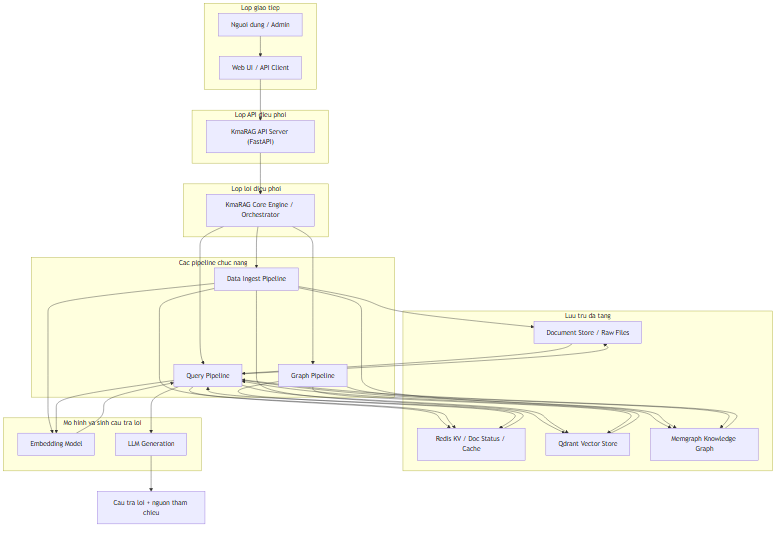
\includegraphics[width=\textwidth,height=0.82\textheight,keepaspectratio]{content/source/RAG/architecture/kmarag_overall_architecture.png}
    \caption{Kiến trúc tổng thể hệ thống KmaRAG}
    \label{fig:rag-overall-architecture}
\end{figure}

Ở lớp giao tiếp, người dùng và quản trị viên thao tác qua Web UI hoặc API client. Phía dưới là \texttt{KmaRAG API Server} viết bằng FastAPI, nơi tiếp nhận request, kiểm tra tham số và định tuyến đến pipeline phù hợp. Từ tài liệu kỹ thuật và mã nguồn có thể xác minh các nhánh chính như upload/scan/reprocess tài liệu, truy vấn non-streaming hoặc streaming, và các thao tác graph management.

Lớp lõi \texttt{KmaRAG Core Engine} đóng vai trò orchestrator, gom toàn bộ các thao tác ingest, query, graph, cache và phối hợp lưu trữ. Từ lõi này, hệ thống tách ra ba pipeline chính. \texttt{Data Ingest Pipeline} xử lý tài liệu thô, sinh chunk, embedding, entity và relation. \texttt{Query Pipeline} lấy câu hỏi, truy hồi dữ liệu từ nhiều nguồn, xây dựng context và gọi LLM để sinh câu trả lời. \texttt{Graph Pipeline} phụ trách cập nhật và khai thác tri thức đồ thị, đồng thời hỗ trợ các thao tác quản trị graph qua API.

Phía dưới các pipeline là lớp lưu trữ đa tầng. \texttt{Redis} được dùng cho KV, trạng thái tài liệu và cache; \texttt{Qdrant} lưu vector để semantic retrieval; \texttt{Memgraph} lưu knowledge graph cho entity và relation; còn \texttt{Document Store} giữ tài liệu gốc hoặc dữ liệu tài liệu đã chuẩn hóa. Trên lớp lưu trữ là lớp mô hình, gồm embedding model để biến văn bản thành biểu diễn ngữ nghĩa và LLM để sinh câu trả lời cuối cùng. Đầu ra của toàn bộ kiến trúc không chỉ là câu trả lời văn bản mà còn gồm nguồn tham chiếu, phù hợp với yêu cầu truy vết của phân hệ RAG.

\section{Thiết kế hai luồng vận hành chính}

Phân hệ RAG có hai luồng vận hành chính: Indexing Flow và Query Flow. Hai luồng này không độc lập hoàn toàn mà sử dụng chung kho dữ liệu, metadata, vector index, graph và trạng thái tài liệu.

Indexing Flow là luồng sản xuất tri thức. Luồng này chạy khi quản trị viên upload tài liệu mới, scan thư mục tài liệu hoặc xử lý lại tài liệu lỗi. Nhiệm vụ của Indexing Flow là biến tài liệu thô thành các đơn vị tri thức có thể truy hồi như full document, chunk, embedding, entity, relation và graph.

Query Flow là luồng tiêu thụ tri thức. Luồng này chạy khi người dùng đặt câu hỏi. Nhiệm vụ của Query Flow là chuẩn hóa câu hỏi, truy hồi bằng chứng từ vector store hoặc graph, xây dựng context và gọi LLM để tạo câu trả lời có căn cứ. Tài liệu Flow report cũng mô tả rõ RAG có hai pipeline chính: Indexing Flow biến tài liệu thô thành chunk, vector, entity, relation và graph; Query Flow biến câu hỏi tự nhiên thành truy vấn, tìm bằng chứng, xây dựng ngữ cảnh và yêu cầu LLM sinh câu trả lời.

\subsection{Indexing Flow}

Indexing Flow là luồng sản xuất tri thức, bắt đầu từ tài liệu thô, đi qua các bước đọc file, kiểm tra định dạng, trích xuất nội dung, đưa vào hàng đợi, chunking, trích xuất entity/relation, ghi graph/vector và cập nhật trạng thái tài liệu.

\begin{figure}[H]
    \centering
    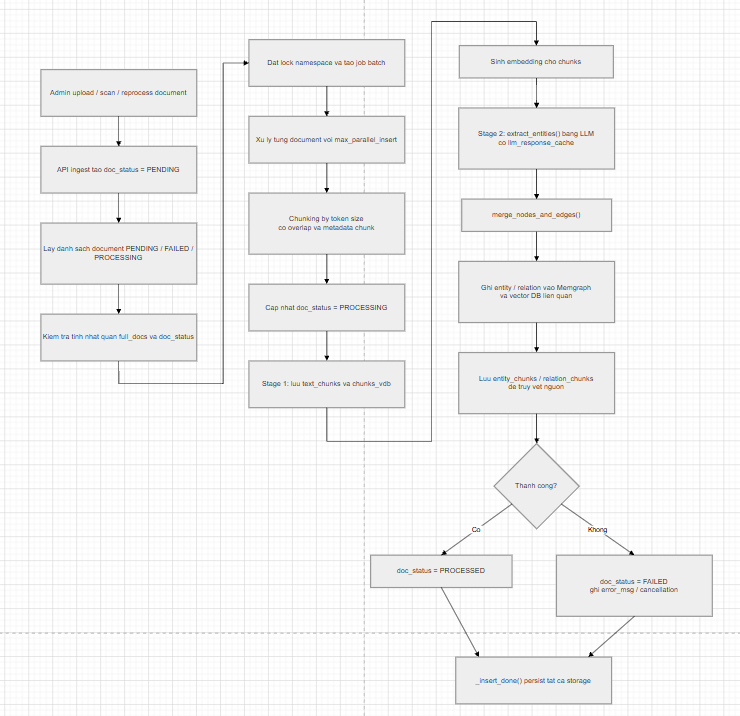
\includegraphics[width=\textwidth,height=0.82\textheight,keepaspectratio]{content/source/RAG/flows/kmarag_indexing_flow.png}
    \caption{Luồng Indexing Flow trong KmaRAG}
    \label{fig:rag-indexing-flow}
\end{figure}

Luồng Indexing có thể mô tả rút gọn như sau:

\begin{center}
\begin{tabular}{c}
Tài liệu thô \\
$\downarrow$ \\
Parse / Preprocess \\
$\downarrow$ \\
Chunking \\
$\downarrow$ \\
Embedding \\
$\downarrow$ \\
Vector Store + Document Store \\
$\downarrow$ \\
Entity / Relation Extraction \\
$\downarrow$ \\
Knowledge Graph \\
$\downarrow$ \\
Doc Status
\end{tabular}
\end{center}

\subsection{Query Flow}

Query Flow bắt đầu từ request \texttt{/query/stream}, sau đó hệ thống validate dữ liệu đầu vào, chuẩn hóa tham số, tạo query parameter cho LLM, kiểm tra mode truy vấn và điều hướng sang các nhánh local, global, hybrid, mix, naive hoặc bypass.

\begin{figure}[H]
    \centering
    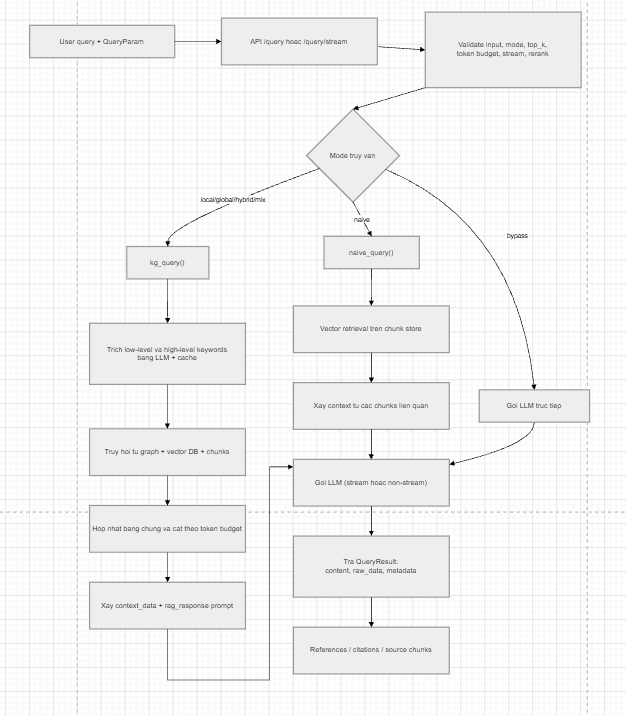
\includegraphics[width=\textwidth,height=0.82\textheight,keepaspectratio]{content/source/RAG/flows/kmarag_query_flow.png}
    \caption{Luồng truy vấn trong KmaRAG}
    \label{fig:rag-query-flow}
\end{figure}

Trong quá trình truy vấn, hệ thống không chỉ truy hồi và sinh câu trả lời theo một đường thẳng. Một số điểm kiểm soát được đặt trong luồng, ví dụ nếu thiếu thực thể thì hỏi lại, nếu không có bằng chứng thì không trả lời khẳng định, nếu mâu thuẫn nguồn thì cần reranking hoặc thông báo mức độ không chắc chắn.

Query Flow có thể mô tả rút gọn như sau:

\begin{center}
\begin{tabular}{c}
Câu hỏi người dùng \\
$\downarrow$ \\
Query Normalization \\
$\downarrow$ \\
Embedding Query \\
$\downarrow$ \\
Vector / Graph Retrieval \\
$\downarrow$ \\
Context Builder \\
$\downarrow$ \\
LLM Generation \\
$\downarrow$ \\
Answer + Citation
\end{tabular}
\end{center}

Điểm quan trọng là Query Flow chỉ hoạt động tốt nếu Indexing Flow tạo ra dữ liệu sạch, có metadata và có chỉ mục đúng. Nếu tài liệu bị parse lỗi, chunk mất ngữ cảnh hoặc metadata thiếu năm áp dụng, hệ thống có thể truy hồi nhầm nguồn và sinh câu trả lời không đáng tin cậy.

\section{Thiết kế Data Ingest và Data Preprocessing}

Data Ingest Pipeline là lớp đầu vào của RAG, chịu trách nhiệm tiếp nhận và xử lý tài liệu. Trong hệ thống tuyển sinh, tài liệu đầu vào có thể là PDF, DOCX, XLSX hoặc các biểu mẫu hành chính. Đây là nhóm dữ liệu không đồng nhất, có thể chứa văn bản, bảng, tiêu đề, danh sách, mã ngành, tổ hợp môn, điểm chuẩn và mốc thời gian.

Trước khi tài liệu được đưa vào kho tri thức, hệ thống phải kiểm tra nguồn dữ liệu, đăng ký ingest, parse nội dung, kiểm tra OCR nếu cần, chuẩn hóa Unicode, kiểm tra metadata và chỉ cho phép các tài liệu đạt chất lượng đi tiếp sang bước chunking và indexing.

\begin{figure}[H]
    \centering
    \includegraphics[width=0.95\textwidth]{content/source/RAG/Pipeline Data Ingest và Data Preprocessing.png}
    \caption{Pipeline data ingest và preprocessing cho kho tri thức RAG tuyển sinh}
    \label{fig:rag-data-ingest-preprocessing}
\end{figure}

Luồng ingest tài liệu quan sát được gồm các bước: admin upload tài liệu hoặc scan thư mục input, pipeline đọc file PDF/DOCX/XLSX, trích xuất văn bản, chuẩn hóa, chia chunks, sinh embedding bằng BAAI/bge-m3, lưu metadata và trạng thái vào RedisDocStatusStorage, lưu vector vào Qdrant và lưu quan hệ tri thức vào Memgraph.

Luồng thiết kế chi tiết:

\begin{center}
\begin{tabular}{c}
Admin upload / scan tài liệu \\
$\downarrow$ \\
Kiểm tra định dạng file \\
$\downarrow$ \\
Parse ná»™i dung \\
$\downarrow$ \\
Làm sạch văn bản \\
$\downarrow$ \\
Chuẩn hóa Unicode, khoảng trắng, tiêu đề, bảng \\
$\downarrow$ \\
Sinh metadata tài liệu \\
$\downarrow$ \\
Chia chunk \\
$\downarrow$ \\
Kiểm tra chất lượng chunk \\
$\downarrow$ \\
Sinh embedding \\
$\downarrow$ \\
Ghi document store, vector store, graph store \\
$\downarrow$ \\
Cập nhật trạng thái processed / pending / failed
\end{tabular}
\end{center}

Mỗi tài liệu cần có metadata tối thiểu:

\begin{itemize}
    \item \texttt{document\_id}, \texttt{file\_name}, \texttt{file\_type}, \texttt{source\_type}.
    \item \texttt{created\_at}, \texttt{updated\_at}, \texttt{status}.
    \item \texttt{chunk\_count}, \texttt{content\_length}, \texttt{checksum}.
    \item \texttt{track\_id}, \texttt{valid\_status}.
\end{itemize}

Mỗi chunk cần có metadata riêng:

\begin{itemize}
    \item \texttt{chunk\_id}, \texttt{document\_id}, \texttt{chunk\_index}.
    \item \texttt{section\_title}, \texttt{page\_number}, \texttt{content}.
    \item \texttt{content\_length}, \texttt{embedding\_model}, \texttt{created\_at}, \texttt{source\_file}.
\end{itemize}

Vai trò của metadata là giúp hệ thống truy vết nguồn, lọc theo năm, loại tài liệu, trạng thái hiệu lực và hỗ trợ citation khi trả lời. Nếu không có metadata, LLM có thể trả lời đúng về mặt ngữ nghĩa nhưng không chứng minh được câu trả lời lấy từ đâu.

\section{Thiết kế Chunking và Metadata}

Chunking là bước chia tài liệu thành các đoạn nhỏ để phục vụ embedding và truy hồi. Nếu chunk quá dài, vector embedding có thể bị loãng nghĩa vì chứa nhiều chủ đề. Nếu chunk quá ngắn, hệ thống có thể mất ngữ cảnh, ví dụ mất quan hệ giữa tên ngành, mã ngành, tổ hợp môn và điểm chuẩn.

Trong hệ thống tuyển sinh, chunk nên được thiết kế theo đơn vị nghĩa thay vì cắt cứng theo số ký tự. Các đơn vị phù hợp gồm:

\begin{itemize}
    \item Một mục trong quy chế tuyển sinh.
    \item Một bảng điểm chuẩn theo năm.
    \item Một nhóm thông tin về một ngành.
    \item Một đoạn mô tả phương thức xét tuyển.
    \item Một phần hướng dẫn hồ sơ nhập học.
    \item Một nhóm dòng trong file Excel tuyển sinh.
\end{itemize}

Ví dụ, với tài liệu điểm chuẩn, chunk không nên tách riêng tên ngành và điểm chuẩn thành hai đoạn khác nhau. Một chunk tốt cần giữ được đầy đủ tên ngành, mã ngành, tổ hợp xét tuyển, điểm chuẩn, năm tuyển sinh, cơ sở đào tạo nếu có và nguồn tài liệu.

Cấu trúc chunk đề xuất:

\begin{table}[H]
\centering
\begin{tabular}{|p{3.8cm}|p{9cm}|}
\hline
\textbf{Trường} & \textbf{Ví dụ} \\
\hline
\texttt{chunk\_id} & \texttt{diem\_chuan\_2025\_001} \\
\hline
\texttt{document\_id} & \texttt{diem\_chuan\_kma\_2017\_2025} \\
\hline
\texttt{section\_title} & Điểm chuẩn năm 2025 \\
\hline
\texttt{content} & Năm 2025, ngành Công nghệ thông tin mã 7480201KMA xét các tổ hợp A00, A01, D01, điểm chuẩn là ... \\
\hline
\texttt{metadata} & \texttt{year}: 2025; \texttt{topic}: \texttt{diem\_chuan}; \texttt{major}: Công nghệ thông tin; \texttt{source\_file}: tài liệu điểm chuẩn \\
\hline
\end{tabular}
\caption{Ví dụ cấu trúc chunk cho dữ liệu điểm chuẩn}
\label{tab:rag-chunk-structure}
\end{table}

Thiết kế chunk tốt giúp retrieval lấy được đúng bằng chứng và giúp LLM không phải suy đoán quan hệ bị thiếu.

\section{Thiết kế Index Layer và các lớp lưu trữ}

Phân hệ RAG không nên chỉ dùng một loại cơ sở dữ liệu. Hệ thống hiện tại đã sử dụng nhiều lớp lưu trữ khác nhau: RedisKVStorage, RedisDocStatusStorage, QdrantVectorDBStorage và MemgraphStorage. Mỗi lớp phục vụ một mục đích riêng.

Trong Index Layer, vector entry không được xem là dữ liệu độc lập. Mỗi kết quả truy hồi từ vector database phải truy ngược được về chunk, metadata và tài liệu gốc để phục vụ citation.

\begin{figure}[H]
    \centering
    \includegraphics[width=0.95\textwidth]{content/source/RAG/Quan hệ giữa document index chunk index metadata index vector database và graph index trong Index Layer của KmaRAG.png}
    \caption{Quan hệ giữa document index, chunk index, metadata index và vector database}
    \label{fig:rag-index-layer-relation}
\end{figure}

Thiết kế các lớp lưu trữ:

\begin{table}[H]
\centering
\begin{tabular}{|p{4.3cm}|p{8.7cm}|}
\hline
\textbf{Kho lưu trữ} & \textbf{Vai trò} \\
\hline
Document Store & Lưu tài liệu gốc, nội dung đã chuẩn hóa và chunk text. \\
\hline
RedisDocStatusStorage & Theo dõi trạng thái xử lý tài liệu. \\
\hline
QdrantVectorDBStorage & Lưu vector embedding phục vụ semantic search. \\
\hline
MemgraphStorage & Lưu entity, relation và knowledge graph. \\
\hline
RedisKVStorage & Lưu cache, key-value metadata và kết quả trung gian. \\
\hline
\end{tabular}
\caption{Các lớp lưu trữ trong phân hệ RAG}
\label{tab:rag-storage-layers}
\end{table}

Ưu điểm của thiết kế đa tầng là mỗi loại dữ liệu được lưu ở nơi phù hợp. Vector database tối ưu cho tìm kiếm tương đồng, nhưng không phù hợp để lưu đầy đủ tài liệu gốc. Graph database phù hợp với quan hệ entity-relation, nhưng không thay thế được chunk text. Redis phù hợp với trạng thái nhanh và cache, nhưng không phải kho tri thức chính.

\section{Thiết kế Embedding Layer}

Embedding Layer có nhiệm vụ chuyển câu hỏi, chunk, entity và relation thành vector số để truy hồi theo ngữ nghĩa. Trong hệ thống hiện tại, embedding model được ghi nhận là BAAI/bge-m3. Đây là mô hình phù hợp cho truy hồi đa ngôn ngữ và có thể xử lý tốt các truy vấn tiếng Việt trong miền tuyển sinh.

Trong Indexing Flow, embedding được sinh cho các chunk sau khi đã qua preprocessing. Trong thiết kế graph-based RAG, embedding cũng có thể được sinh cho entity và relation. Tài liệu Flow report nhấn mạnh bge-m3 được dùng để sinh vector cho chunk, entity và relation; đồng thời query cũng phải dùng cùng embedding model để bảo đảm vector có thể so sánh trong cùng không gian.

Công thức mô tả:

\begin{equation}
v_i = E(d_i), \qquad v_q = E(q)
\end{equation}

Trong đó:

\begin{itemize}
    \item $E$ là hàm embedding.
    \item $d_i$ là chunk tài liệu thứ $i$.
    \item $q$ là câu hỏi người dùng.
    \item $v_i$ là vector của chunk.
    \item $v_q$ là vector của câu hỏi.
\end{itemize}

Độ tương đồng cosine được tính như sau:

\begin{equation}
sim(q, d_i) = \frac{v_q \cdot v_i}{\|v_q\| \|v_i\|}
\end{equation}

Khi người dùng hỏi ``CNTT có xét học bạ không?'', hệ thống cần truy hồi được chunk chứa các cụm tương đương như ``Công nghệ thông tin'', ``phương thức xét tuyển'', ``xét kết quả học tập THPT'' hoặc ``xét học bạ''. Điều này cho thấy embedding giúp hệ thống vượt qua giới hạn của keyword matching. Tuy nhiên, embedding cũng cần được kiểm soát bằng metadata và keyword search, vì các câu hỏi tuyển sinh thường chứa mã ngành, năm, tổ hợp môn và con số.

Các điểm kiểm soát của Embedding Layer:

\begin{itemize}
    \item Indexing và query phải dùng cùng model embedding.
    \item Vector dimension phải khớp với schema của vector database.
    \item Cần lưu \texttt{embedding\_model}, \texttt{embedding\_version} và \texttt{created\_at}.
    \item Cần rebuild vector index khi đổi model embedding.
    \item Cần cache query embedding cho câu hỏi lặp.
    \item Không embedding dữ liệu parse lỗi hoặc OCR confidence thấp.
\end{itemize}

\section{Thiết kế Knowledge Graph}

Knowledge Graph là lớp mở rộng giúp RAG không chỉ truy hồi đoạn văn gần nghĩa, mà còn hiểu quan hệ giữa các thực thể. Trong bài toán tuyển sinh, các entity quan trọng gồm ngành học, mã ngành, tổ hợp môn, phương thức xét tuyển, điểm chuẩn, học phí, năm tuyển sinh, cơ sở đào tạo và loại tài liệu.

Sau khi chunk được chuẩn hóa, hệ thống có thể trích xuất entity, chuẩn hóa entity, trích xuất relation, xử lý xung đột và ghi vào graph store. Các entity và relation này được liên kết ngược về chunk và tài liệu gốc để bảo đảm khả năng truy vết.

\begin{figure}[H]
    \centering
    \includegraphics[width=0.9\textwidth]{content/source/RAG/Pipeline xây dựng Knowledge Graph từ chunk đã chuẩn hóa.png}
    \caption{Pipeline xây dựng Knowledge Graph từ chunk đã chuẩn hóa}
    \label{fig:rag-knowledge-graph-pipeline}
\end{figure}

Ví dụ entity:

\begin{itemize}
    \item Ngành: Công nghệ thông tin.
    \item Mã ngành: 7480201KMA.
    \item Tổ hợp: A00, A01, D01.
    \item Phương thức: xét điểm thi THPT, xét học bạ.
    \item Năm: 2025, 2026.
    \item Tài liệu: Quy chế tuyển sinh 2026.
\end{itemize}

Ví dụ relation:

\begin{itemize}
    \item Công nghệ thông tin -- có mã ngành -- 7480201KMA.
    \item Công nghệ thông tin -- xét tổ hợp -- A00.
    \item Công nghệ thông tin -- xét tổ hợp -- A01.
    \item Công nghệ thông tin -- xét tổ hợp -- D01.
    \item Công nghệ thông tin -- có điểm chuẩn năm 2025 -- 24.42.
    \item Quy chế tuyển sinh 2026 -- quy định -- phương thức xét tuyển.
\end{itemize}

Flow report mô tả rõ giá trị của Knowledge Graph: vector search trả lời tốt câu hỏi gần nghĩa, nhưng graph giúp trả lời các câu hỏi có quan hệ, có điều kiện và cần tổng hợp; ví dụ thay vì chỉ tìm đoạn nói về ``D01'', hệ thống có thể tìm các ngành có relation với tổ hợp D01, sau đó lấy chunk nguồn để trích dẫn.

Thiết kế schema rút gọn:

\begin{table}[H]
\centering
\begin{tabular}{|p{3.8cm}|p{9cm}|}
\hline
\textbf{Đối tượng} & \textbf{Thuộc tính} \\
\hline
Entity & \texttt{entity\_id}, \texttt{canonical\_name}, \texttt{aliases}, \texttt{entity\_type}, \texttt{description}, \texttt{source\_chunk\_id}, \texttt{document\_id}, \texttt{status}. \\
\hline
Relation & \texttt{relation\_id}, \texttt{source\_entity}, \texttt{target\_entity}, \texttt{relation\_type}, \texttt{description}, \texttt{source\_chunk\_id}, \texttt{confidence}, \texttt{status}. \\
\hline
\end{tabular}
\caption{Schema rút gọn cho entity và relation trong Knowledge Graph}
\label{tab:rag-kg-schema}
\end{table}

Knowledge Graph đặc biệt hữu ích với các câu hỏi như: những ngành nào xét D01, ngành Công nghệ thông tin có xét học bạ không, mã ngành 7480201 thuộc ngành nào, ngành An toàn thông tin có những tổ hợp nào hoặc điểm chuẩn ngành này qua các năm thay đổi thế nào.

\section{Thiết kế Retrieval và các mode truy vấn}

Query Flow là luồng xử lý trực tuyến khi người dùng đặt câu hỏi. Đây là phần trực tiếp quyết định chất lượng trải nghiệm hỏi đáp của người dùng.

Luồng Query Flow đề xuất:

\begin{center}
\begin{tabular}{c}
Người dùng đặt câu hỏi \\
$\downarrow$ \\
Nhận query từ frontend/backend \\
$\downarrow$ \\
Chuẩn hóa câu hỏi \\
$\downarrow$ \\
Phân tích keyword/entity \\
$\downarrow$ \\
Chọn mode truy vấn \\
$\downarrow$ \\
Embedding query \\
$\downarrow$ \\
Truy hồi chunk/entity/relation \\
$\downarrow$ \\
Reranking nếu có \\
$\downarrow$ \\
Context assembly \\
$\downarrow$ \\
Prompt assembly \\
$\downarrow$ \\
LLM generation \\
$\downarrow$ \\
Hậu xử lý citation \\
$\downarrow$ \\
Trả câu trả lời cho người dùng
\end{tabular}
\end{center}

Bước chuẩn hóa query cần xử lý các vấn đề như viết tắt CNTT thành Công nghệ thông tin, nhận diện mã ngành 7480201KMA, nhận diện tổ hợp môn A00, A01, D01, chuẩn hóa cụm ``năm nay'' thành năm tuyển sinh hiện hành, sửa lỗi chính tả nhẹ và xử lý câu hỏi nối tiếp dựa vào lịch sử hội thoại.

Ví dụ:

\begin{itemize}
    \item Query gốc: ``CNTT năm nay xét học bạ không?''
    \item Sau chuẩn hóa: ``Ngành Công nghệ thông tin tuyển sinh năm 2026 có xét học bạ không?''
\end{itemize}

Để phù hợp với nhiều loại câu hỏi, RAG nên hỗ trợ nhiều mode truy vấn thay vì chỉ dùng một chiến lược duy nhất.

\begin{table}[H]
\centering
\begin{tabular}{|p{3.2cm}|p{9.6cm}|}
\hline
\textbf{Mode} & \textbf{Mô tả} \\
\hline
Naive mode & Truy hồi trực tiếp trên chunks vector database bằng vector search. \\
\hline
Local mode & Truy hồi entity liên quan, sau đó mở rộng quan hệ lân cận trong graph. \\
\hline
Global mode & Truy hồi relation hoặc chủ đề rộng trong graph. \\
\hline
Hybrid mode & Kết hợp entity retrieval và relation retrieval. \\
\hline
Mix mode & Kết hợp graph retrieval với chunk vector retrieval. \\
\hline
Bypass mode & Gọi LLM trực tiếp, chỉ dùng cho câu hỏi giao tiếp chung, không dùng cho dữ liệu tuyển sinh. \\
\hline
\end{tabular}
\caption{Các mode truy vấn đề xuất cho phân hệ RAG}
\label{tab:rag-query-modes}
\end{table}

Bảng lựa chọn mode:

\begin{table}[H]
\centering
\begin{tabular}{|p{6cm}|p{6.8cm}|}
\hline
\textbf{Câu hỏi} & \textbf{Mode phù hợp} \\
\hline
``CNTT có xét học bạ không?'' & local / mix \\
\hline
``Các ngành nào xét D01?'' & global / mix \\
\hline
``Mã ngành 7480201 xét A00 không?'' & hybrid \\
\hline
``Điểm chuẩn ngành ATTT năm 2025?'' & naive / mix \\
\hline
``So sánh xét học bạ và xét điểm thi'' & global / mix \\
\hline
``Viết lời chào cho chatbot'' & bypass \\
\hline
\end{tabular}
\caption{Gợi ý lựa chọn mode truy vấn theo loại câu hỏi}
\label{tab:rag-mode-selection}
\end{table}

Trong hệ thống tuyển sinh, mix mode thường an toàn nhất cho câu hỏi quan trọng vì vừa dùng graph để hiểu quan hệ, vừa dùng chunk nguồn để trích dẫn. Tuy nhiên, mode này có thể tốn nhiều thời gian và context token hơn, nên cần cân nhắc giữa chất lượng, độ trễ và chi phí.

\section{Thiết kế Context Builder, Prompt và LLM Generation}

Context Builder là lớp chọn và sắp xếp bằng chứng trước khi gửi cho LLM. Đây là bước rất quan trọng vì LLM chỉ nên trả lời dựa trên context đã được cung cấp.

Đầu vào của Context Builder gồm câu hỏi đã chuẩn hóa, danh sách chunk truy hồi, danh sách entity liên quan, danh sách relation liên quan, metadata tài liệu, điểm similarity và trạng thái hiệu lực tài liệu. Đầu ra cần là context ngắn gọn, ít trùng lặp, đủ bằng chứng, có metadata nguồn và phù hợp với giới hạn token.

Nguyên tắc chọn context:

\begin{itemize}
    \item Ưu tiên tài liệu đúng năm tuyển sinh.
    \item Ưu tiên tài liệu có trạng thái processed/active.
    \item Ưu tiên chunk có similarity cao.
    \item Ưu tiên chunk có metadata khớp entity trong câu hỏi.
    \item Loại bỏ chunk trùng hoặc gần trùng.
    \item Không đưa tài liệu failed/needs\_review vào context chính thức.
    \item Giữ nguồn \texttt{chunk\_id}/\texttt{document\_id} để citation.
\end{itemize}

Ví dụ với câu hỏi ``Công nghệ thông tin năm 2025 lấy bao nhiêu điểm?'', context nên gồm chunk từ tài liệu điểm chuẩn, dòng chứa ngành Công nghệ thông tin, mã ngành, tổ hợp xét tuyển, điểm chuẩn năm 2025 và nguồn tài liệu. Không nên đưa thêm các chunk nói về học phí, chương trình đào tạo hoặc quy chế thi nếu chúng không trực tiếp trả lời câu hỏi.

Sau khi context được xây dựng, hệ thống tạo prompt để gọi LLM. Trong RAG, LLM không được xem là nguồn tri thức độc lập. LLM chỉ có nhiệm vụ diễn đạt câu trả lời dựa trên bằng chứng đã truy hồi.

Prompt nên có cấu trúc:

\begin{itemize}
    \item System instruction: chatbot tư vấn tuyển sinh, chỉ trả lời dựa trên context được cung cấp.
    \item User question: câu hỏi gốc hoặc câu hỏi đã chuẩn hóa.
    \item Retrieved context: các chunk, entity, relation và metadata đã chọn.
    \item Yêu cầu trả lời: ngắn gọn, rõ ràng, nêu đúng năm áp dụng, trích dẫn nguồn nếu có và nói chưa đủ dữ liệu nếu context không đủ.
\end{itemize}

Nếu context có đủ dữ liệu, hệ thống có thể trả lời: ``Ngành Công nghệ thông tin năm 2025 có điểm chuẩn là ... theo tài liệu điểm chuẩn của Học viện.'' Nếu context không đủ dữ liệu, hệ thống nên trả lời: ``Mình chưa tìm thấy thông tin đủ rõ trong kho tài liệu hiện tại về nội dung này. Bạn có thể cho biết thêm năm tuyển sinh hoặc ngành cụ thể không?''

Tài liệu tổng hợp cũng nhấn mạnh Query Flow cần biết khi nào đủ bằng chứng để trả lời, khi nào cần hỏi lại và khi nào phải thừa nhận thiếu dữ liệu. Đây là nguyên tắc quan trọng trong chatbot tuyển sinh để giữ độ tin cậy của thông tin về ngành, phương thức xét tuyển, tổ hợp môn, học phí, điểm chuẩn và mốc thời gian.

\section{Thiết kế Citation và truy vết nguồn}

Citation là cơ chế giúp người dùng và quản trị viên kiểm chứng câu trả lời. Một câu trả lời RAG tốt không chỉ đúng nội dung mà còn phải cho biết nguồn lấy từ đâu.

Mỗi câu trả lời nên gắn với:

\begin{itemize}
    \item \texttt{document\_id}.
    \item \texttt{document\_name}.
    \item \texttt{chunk\_id}.
    \item \texttt{page\_number} hoặc \texttt{section\_title} nếu có.
    \item \texttt{updated\_at}.
    \item \texttt{valid\_status}.
\end{itemize}

Ví dụ: nguồn là tài liệu điểm chuẩn của Học viện, chunk 2, cập nhật ngày 14/04/2026. Với các câu trả lời có nhiều mệnh đề, mỗi mệnh đề quan trọng nên có bằng chứng riêng. Ví dụ, nếu trả lời vừa có điểm chuẩn, vừa có tổ hợp xét tuyển, vừa có mã ngành, hệ thống cần bảo đảm cả ba thông tin đều xuất hiện trong context.

Thiết kế citation giúp người dùng tin tưởng hơn, quản trị viên kiểm tra được nguồn, dễ phát hiện lỗi parse hoặc lỗi retrieval, dễ cập nhật tài liệu khi thông tin thay đổi và giảm rủi ro LLM tự sinh thông tin không có căn cứ.

\section{Tích hợp RAG với Rasa}

Trong hệ thống tổng thể, Rasa và RAG cần phối hợp với nhau. Rasa xử lý intent, hội thoại, fallback và các câu hỏi định sẵn. RAG xử lý các câu hỏi cần truy xuất tài liệu.

Có thể thiết kế luồng tích hợp như sau:

\begin{center}
\begin{tabular}{p{12cm}}
Người dùng gửi câu hỏi \\
$\downarrow$ \\
Rasa NLU phân loại intent \\
$\downarrow$ \\
Nếu intent rõ và thuộc FAQ: Rasa trả lời bằng domain/action \\
$\downarrow$ \\
Nếu intent cần tài liệu: Custom action gọi RAG API \\
$\downarrow$ \\
Nếu confidence thấp: fallback hoặc hỏi lại, có thể chuyển sang RAG nếu câu hỏi có dạng truy vấn tài liệu
\end{tabular}
\end{center}

Các intent nên chuyển sang RAG:

\begin{itemize}
    \item \texttt{hoi\_diem\_chuan}.
    \item \texttt{hoi\_phuong\_thuc\_tuyen\_sinh}.
    \item \texttt{hoi\_chuong\_trinh\_dao\_tao}.
    \item \texttt{hoi\_quy\_che}.
    \item \texttt{hoi\_hoc\_phi}.
    \item \texttt{hoi\_ho\_so\_nhap\_hoc}.
    \item \texttt{hoi\_van\_ban\_bieu\_mau}.
    \item \texttt{hoi\_nguon\_tai\_lieu}.
\end{itemize}

Custom action có thể gọi endpoint \texttt{/v1/chat/completions} hoặc \texttt{/v1/chunks}. Rasa giữ vai trò điều phối hội thoại, còn RAG giữ vai trò tìm bằng chứng và sinh câu trả lời theo tài liệu. Điều này giúp hệ thống tận dụng ưu điểm của cả hai: Rasa kiểm soát luồng, RAG mở rộng tri thức.

\section{Kiểm thử và đánh giá phân hệ RAG}

Đánh giá RAG cần thực hiện trên cả hai lớp: chất lượng truy hồi và chất lượng câu trả lời. Truy hồi đúng nhưng prompt kém có thể tạo câu trả lời khó hiểu; ngược lại, prompt tốt nhưng truy hồi sai tài liệu sẽ khiến câu trả lời sai căn cứ.

\begin{table}[H]
\centering
\begin{tabular}{|p{4cm}|p{8.8cm}|}
\hline
\textbf{Nhóm đánh giá} & \textbf{Tiêu chí} \\
\hline
Chất lượng truy hồi & Truy hồi đúng tài liệu, đúng năm, đúng ngành, đúng loại thông tin và đúng đoạn chứa câu trả lời. \\
\hline
Chất lượng context & Context đủ thông tin, ít nhiễu, không trùng lặp và giữ được nguồn tham chiếu. \\
\hline
Chất lượng câu trả lời & Trả lời đúng trọng tâm, dễ hiểu, không tự tạo thông tin và có nguồn khi cần. \\
\hline
Khả năng vận hành & Tài liệu mới được xử lý ổn định, trạng thái rõ ràng, có khả năng xử lý lại khi lỗi. \\
\hline
Độ tin cậy & Hệ thống biết từ chối khi không có bằng chứng, biết cảnh báo khi nguồn cũ hoặc mâu thuẫn. \\
\hline
\end{tabular}
\caption{Tiêu chí đánh giá chất lượng phân hệ RAG}
\label{tab:rag-evaluation-criteria}
\end{table}

Bộ kiểm thử RAG nên bao gồm các nhóm câu hỏi về điểm chuẩn, ngành đào tạo, phương thức xét tuyển, hồ sơ nhập học, chính sách ưu tiên, học phí, chương trình đào tạo và các câu hỏi không có trong tài liệu. Nhóm câu hỏi không có trong tài liệu đặc biệt quan trọng vì giúp kiểm tra khả năng từ chối trả lời khi thiếu bằng chứng.

\section{Kết luận chương}

Chương này đã trình bày vai trò, kiến trúc và thiết kế chi tiết của phân hệ RAG trong hệ thống chatbot tư vấn tuyển sinh. RAG được thiết kế như lớp tri thức động, giúp hệ thống khai thác tài liệu tuyển sinh, chương trình đào tạo, điểm chuẩn, quy chế và biểu mẫu để trả lời các câu hỏi cần căn cứ thực tế.

Về vận hành, phân hệ RAG gồm hai luồng chính: Indexing Flow dùng để biến tài liệu thô thành chunk, embedding, metadata và knowledge graph; Query Flow dùng để chuẩn hóa câu hỏi, truy hồi bằng chứng, xây dựng context và gọi LLM sinh câu trả lời có citation. Các lớp như Data Ingest, Chunking, Embedding, Index Layer, Knowledge Graph, Retrieval, Context Builder, Prompt Assembly và Citation được tách riêng để dễ kiểm thử, mở rộng và kiểm soát lỗi.

Khi tích hợp với Rasa, RAG giúp chatbot vừa giữ được khả năng điều phối hội thoại theo intent, vừa trả lời được các câu hỏi có nội dung phụ thuộc tài liệu thực tế. Thiết kế này phù hợp với bài toán tuyển sinh, nơi thông tin thay đổi theo năm và cần khả năng truy vết nguồn rõ ràng.



\chapter{THIẾT KẾ API HỆ THỐNG}

Chương này trình bày thiết kế API cho hệ thống chatbot tư vấn tuyển sinh. API đóng vai trò là lớp trung gian kết nối giữa giao diện người dùng, backend, Rasa Server, Action Server, cơ sở dữ liệu tuyển sinh và phân hệ RAG. Thông qua API, hệ thống có thể tiếp nhận câu hỏi từ người dùng, xử lý xác thực, quản lý dữ liệu huấn luyện chatbot, vận hành mô hình Rasa, truy xuất dữ liệu tuyển sinh và gọi kho tri thức khi cần trả lời các câu hỏi phức tạp.

Hệ thống API được thiết kế theo hướng RESTful, sử dụng đường dẫn có cấu trúc rõ ràng, hỗ trợ phân quyền và dễ mở rộng. Các API chính được đặt dưới tiền tố \texttt{/api/v1}. Dữ liệu trao đổi giữa client và server sử dụng định dạng JSON. Với các chức năng chat thời gian thực, hệ thống có thể sử dụng cơ chế streaming để trả lời từng phần, giúp cải thiện trải nghiệm người dùng.

\section{Nguyên tắc thiết kế API}

API của hệ thống được thiết kế dựa trên các nguyên tắc sau:

\begin{itemize}
    \item \textbf{Phân tách chức năng rõ ràng:} mỗi nhóm API phụ trách một nghiệp vụ riêng như xác thực, quản lý intent, quản lý rule, chat, huấn luyện mô hình hoặc truy vấn RAG.
    \item \textbf{Thống nhất phương thức HTTP:} \texttt{GET} dùng để truy vấn dữ liệu, \texttt{POST} dùng để tạo mới hoặc thực hiện hành động, \texttt{PUT} dùng để cập nhật, \texttt{DELETE} dùng để xóa và \texttt{PATCH} dùng cho các cập nhật trạng thái như khôi phục bản ghi.
    \item \textbf{Hỗ trợ phân trang:} các API lấy danh sách như intent, rule, action và response đều cần hỗ trợ phân trang, tìm kiếm và lọc trạng thái.
    \item \textbf{Hỗ trợ xóa mềm và khôi phục:} dữ liệu quản trị chatbot có thể xóa mềm để tránh mất dữ liệu trong quá trình vận hành.
    \item \textbf{Bảo mật bằng xác thực:} các API quản trị yêu cầu người dùng đăng nhập và có quyền phù hợp.
    \item \textbf{Dễ tích hợp với Rasa và RAG:} các API phải hỗ trợ Action Server gọi dữ liệu tuyển sinh hoặc gọi phân hệ RAG để tạo câu trả lời.
\end{itemize}

Cấu trúc phản hồi API được chuẩn hóa để frontend dễ xử lý. Một phản hồi thành công có thể có dạng:

\begin{verbatim}
{
  "success": true,
  "message": "Success",
  "data": { }
}
\end{verbatim}

Đối với danh sách có phân trang, phản hồi có thể bổ sung thông tin trang hiện tại, tổng số bản ghi và số bản ghi trên mỗi trang:

\begin{verbatim}
{
  "success": true,
  "data": {
    "items": [],
    "page": 1,
    "pageSize": 10,
    "totalItems": 100,
    "totalPages": 10
  }
}
\end{verbatim}

\section{Thiết kế API xác thực người dùng}

Nhóm API xác thực có nhiệm vụ quản lý đăng nhập, đăng ký và xác thực tài khoản. Đây là nhóm API nền tảng để bảo vệ các chức năng quản trị và cá nhân hóa trải nghiệm người dùng.

\begin{longtable}{|p{3cm}|p{5cm}|p{7cm}|}
\hline
\textbf{Phương thức} & \textbf{Endpoint} & \textbf{Mô tả} \\
\hline
\texttt{POST} & \texttt{/v1/auth/login} & Đăng nhập bằng email và mật khẩu. \\
\hline
\texttt{POST} & \texttt{/v1/auth/register} & Đăng ký tài khoản mới. \\
\hline
\texttt{POST} & \texttt{/v1/auth/verify-email} & Xác thực email bằng mã OTP. \\
\hline
\end{longtable}

Khi đăng nhập thành công, hệ thống trả về token xác thực. Token này được frontend lưu trữ và gửi kèm trong các request cần bảo vệ. Các API quản trị như quản lý intent, rule, action, response và huấn luyện chatbot yêu cầu token hợp lệ.

Ví dụ request đăng nhập:

\begin{verbatim}
POST /api/v1/auth/login

{
  "email": "admin@example.com",
  "password": "123456"
}
\end{verbatim}

Ví dụ response:

\begin{verbatim}
{
  "success": true,
  "message": "Login successfully",
  "data": {
    "accessToken": "...",
    "refreshToken": "...",
    "profile": {
      "id": "user-id",
      "email": "admin@example.com",
      "role": "Admin"
    }
  }
}
\end{verbatim}

\section{Thiết kế API quản lý dữ liệu Rasa}

Nhóm API quản lý dữ liệu Rasa cho phép quản trị viên thao tác với các thành phần huấn luyện của chatbot như intent, rule, response và action. Việc đưa các thành phần này lên giao diện quản trị giúp người quản trị có thể cập nhật dữ liệu hội thoại mà không cần chỉnh sửa trực tiếp các file cấu hình của Rasa.

\subsection{API quản lý Intent}

Intent là ý định của người dùng được Rasa NLU nhận diện từ câu hỏi đầu vào. API quản lý intent cho phép thêm, sửa, xóa và khôi phục intent.

\begin{longtable}{|p{3cm}|p{5cm}|p{7cm}|}
\hline
\textbf{Phương thức} & \textbf{Endpoint} & \textbf{Mô tả} \\
\hline
\texttt{GET} & \texttt{/v1/intent} & Lấy danh sách intent có phân trang. \\
\hline
\texttt{POST} & \texttt{/v1/intent} & Tạo intent mới. \\
\hline
\texttt{GET} & \texttt{/v1/intent/\{id\}} & Lấy chi tiết intent theo id. \\
\hline
\texttt{PUT} & \texttt{/v1/intent/\{id\}} & Cập nhật intent. \\
\hline
\texttt{DELETE} & \texttt{/v1/intent/\{id\}/soft} & Xóa mềm intent. \\
\hline
\texttt{DELETE} & \texttt{/v1/intent/\{id\}/hard} & Xóa vĩnh viễn intent. \\
\hline
\texttt{PATCH} & \texttt{/v1/intent/\{id\}/restore} & Khôi phục intent đã xóa mềm. \\
\hline
\end{longtable}

Dữ liệu intent có thể bao gồm tên intent, danh sách câu ví dụ, trạng thái hoạt động và mô tả. Khi intent được cập nhật, hệ thống cần huấn luyện lại mô hình để thay đổi có hiệu lực.

\subsection{API quản lý Rule}

Rule dùng để định nghĩa các luồng phản hồi cố định trong Rasa. API quản lý rule giúp quản trị viên kiểm soát các kịch bản hội thoại có tính xác định cao.

\begin{longtable}{|p{3cm}|p{5cm}|p{7cm}|}
\hline
\textbf{Phương thức} & \textbf{Endpoint} & \textbf{Mô tả} \\
\hline
\texttt{GET} & \texttt{/v1/rule} & Lấy danh sách rule có phân trang. \\
\hline
\texttt{POST} & \texttt{/v1/rule} & Tạo rule mới. \\
\hline
\texttt{GET} & \texttt{/v1/rule/\{id\}} & Lấy chi tiết rule. \\
\hline
\texttt{PUT} & \texttt{/v1/rule/\{id\}} & Cập nhật rule. \\
\hline
\texttt{DELETE} & \texttt{/v1/rule/\{id\}/soft} & Xóa mềm rule. \\
\hline
\texttt{DELETE} & \texttt{/v1/rule/\{id\}/hard} & Xóa vĩnh viễn rule. \\
\hline
\texttt{PATCH} & \texttt{/v1/rule/\{id\}/restore} & Khôi phục rule. \\
\hline
\end{longtable}

Mỗi rule thường bao gồm tên rule, intent kích hoạt, action phản hồi và trạng thái sử dụng. Với các câu hỏi phổ biến như hỏi lời chào, hỏi thông tin trường hoặc hỏi hướng dẫn sử dụng chatbot, rule giúp hệ thống phản hồi nhanh và ổn định.

\subsection{API quản lý Response}

Response là các câu trả lời mẫu được Rasa sử dụng trong phần NLG. API quản lý response cho phép thêm và cập nhật nội dung phản hồi mà không cần chỉnh sửa trực tiếp file \texttt{domain.yml}.

\begin{longtable}{|p{3cm}|p{5cm}|p{7cm}|}
\hline
\textbf{Phương thức} & \textbf{Endpoint} & \textbf{Mô tả} \\
\hline
\texttt{GET} & \texttt{/v1/my-response} & Lấy danh sách response có phân trang. \\
\hline
\texttt{POST} & \texttt{/v1/my-response} & Tạo response mới. \\
\hline
\texttt{GET} & \texttt{/v1/my-response/\{id\}} & Lấy chi tiết response. \\
\hline
\texttt{PUT} & \texttt{/v1/my-response/\{id\}} & Cập nhật response. \\
\hline
\texttt{DELETE} & \texttt{/v1/my-response/\{id\}/soft} & Xóa mềm response. \\
\hline
\texttt{DELETE} & \texttt{/v1/my-response/\{id\}/hard} & Xóa vĩnh viễn response. \\
\hline
\texttt{PATCH} & \texttt{/v1/my-response/\{id\}/restore} & Khôi phục response. \\
\hline
\end{longtable}

Mỗi response có thể chứa tên response, nội dung câu trả lời, biến động nếu có và trạng thái hoạt động. Ví dụ, response \texttt{utter\_greet} có thể chứa nhiều biến thể câu chào để chatbot trả lời tự nhiên hơn.

\begin{figure}[H]
    \centering
    \includegraphics[width=\textwidth,height=0.78\textheight,keepaspectratio]{content/source/mermaid_sequence/IMG/Luồng quản lý intent entity response rule story action.png}
    \caption{Sequence Diagram luồng quản lý intent, entity, response, rule, story và action}
    \label{fig:seq-manage-rasa-training-data}
\end{figure}

\begin{figure}[H]
    \centering
    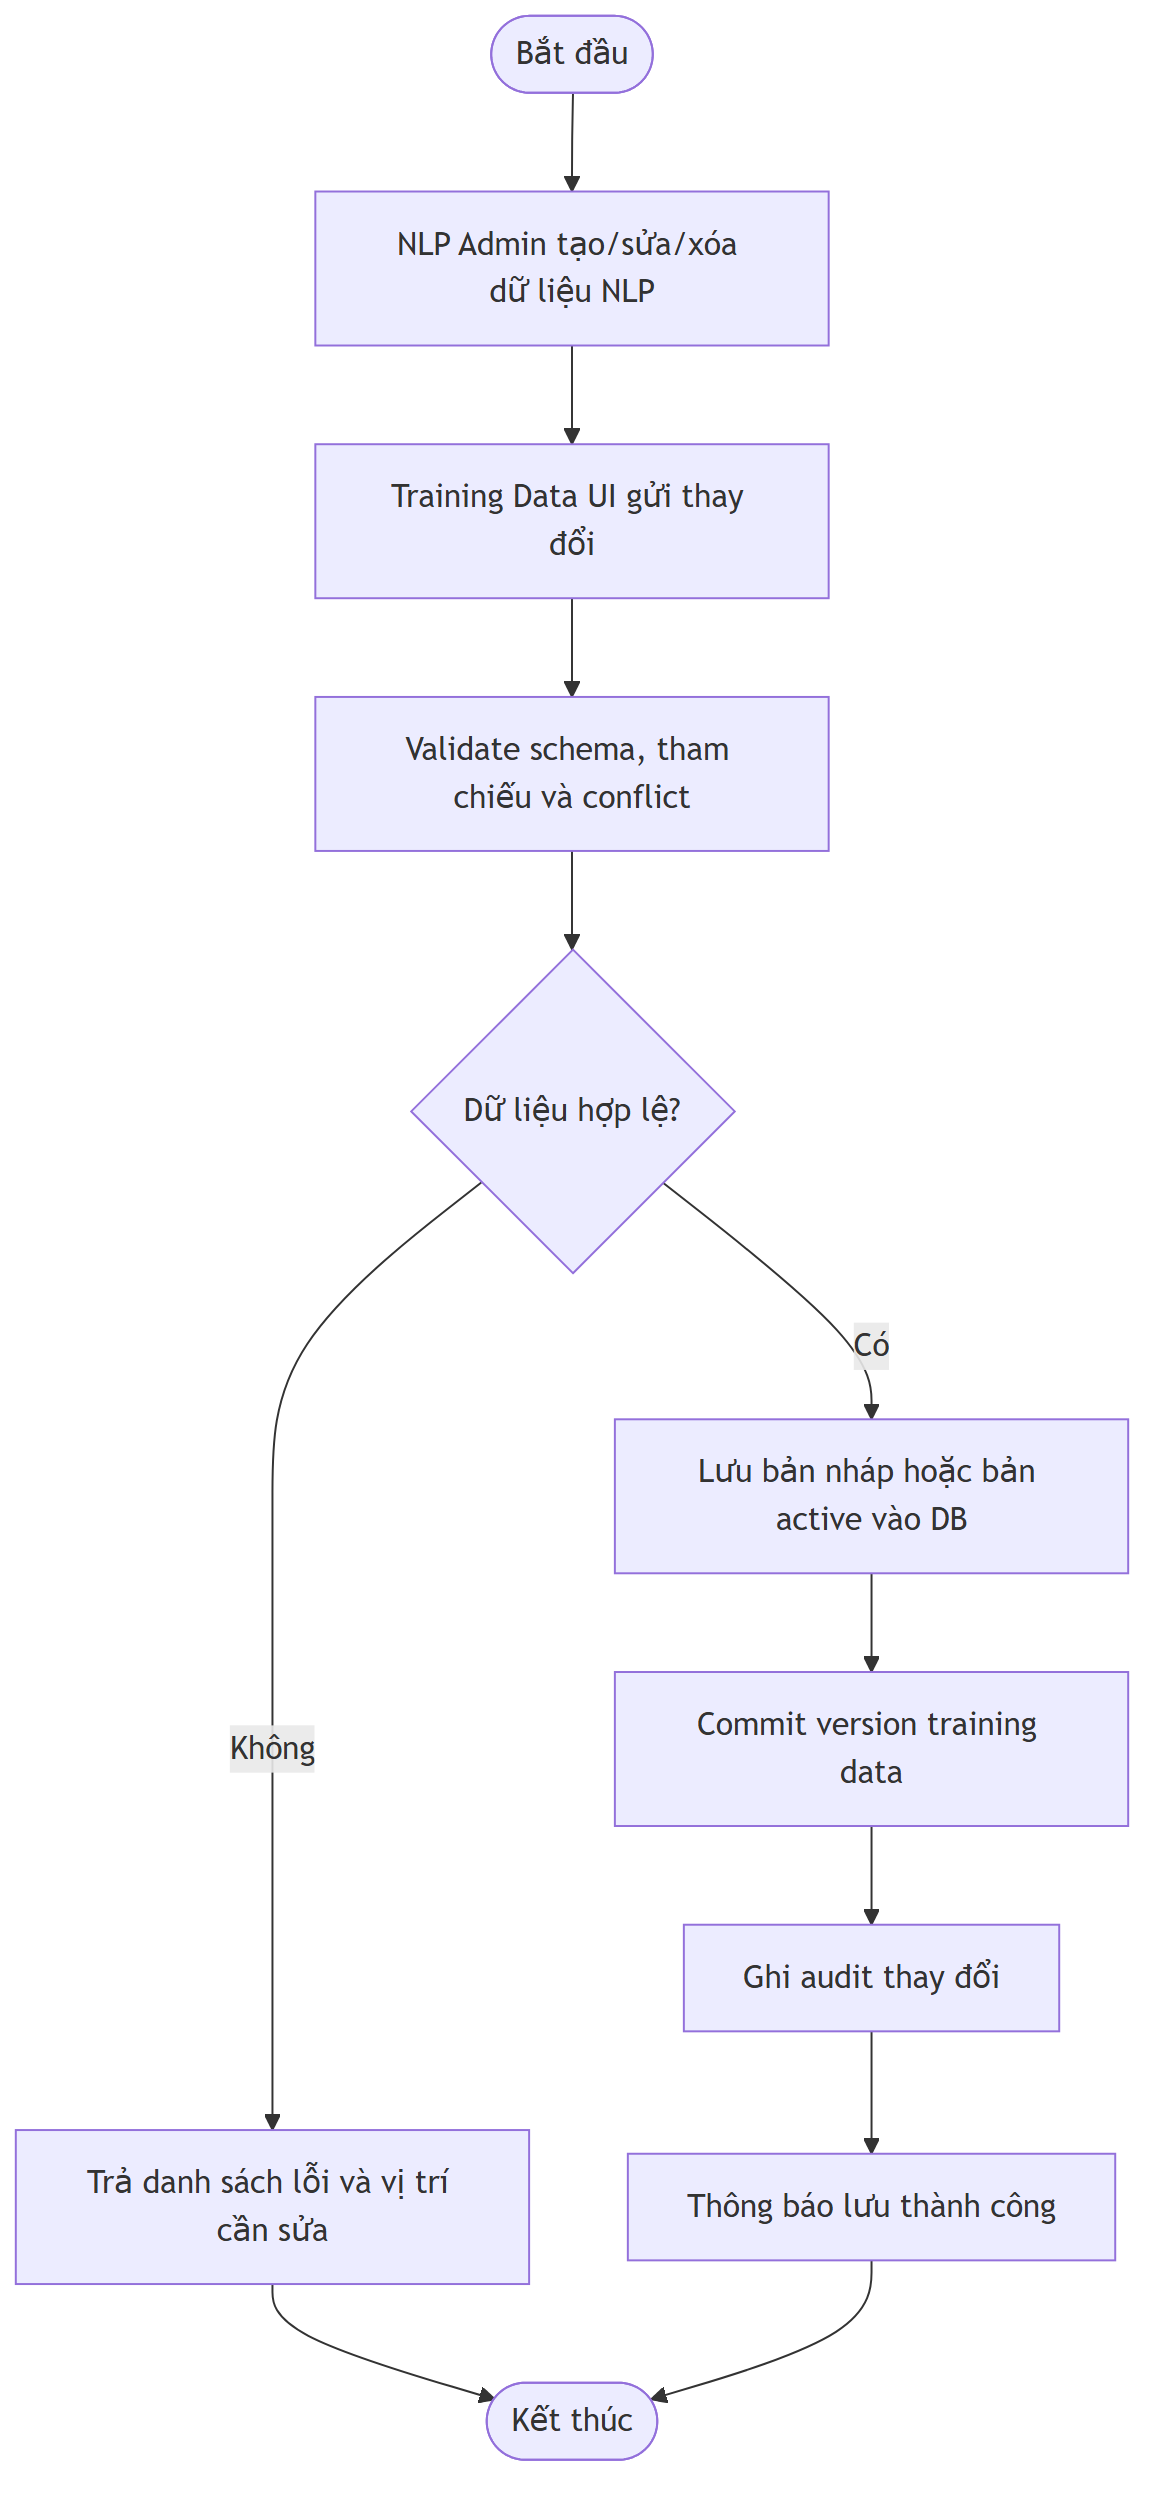
\includegraphics[width=\textwidth,height=0.78\textheight,keepaspectratio]{content/source/mermaid_activity/act_05.png}
    \caption{Activity Diagram luồng quản lý intent, entity, response, rule, story và action}
    \label{fig:act-manage-rasa-training-data}
\end{figure}

\subsection{API quản lý Action}

Action là hành động mà Rasa thực hiện sau khi nhận diện intent và trạng thái hội thoại. Action có thể là câu trả lời tĩnh hoặc custom action gọi sang backend để lấy dữ liệu.

\begin{longtable}{|p{3cm}|p{5cm}|p{7cm}|}
\hline
\textbf{Phương thức} & \textbf{Endpoint} & \textbf{Mô tả} \\
\hline
\texttt{GET} & \texttt{/v1/action} & Lấy danh sách action có phân trang. \\
\hline
\texttt{POST} & \texttt{/v1/action} & Tạo action mới. \\
\hline
\texttt{GET} & \texttt{/v1/action/\{id\}} & Lấy chi tiết action. \\
\hline
\texttt{PUT} & \texttt{/v1/action/\{id\}} & Cập nhật action. \\
\hline
\texttt{DELETE} & \texttt{/v1/action/\{id\}/soft} & Xóa mềm action. \\
\hline
\texttt{DELETE} & \texttt{/v1/action/\{id\}/hard} & Xóa vĩnh viễn action. \\
\hline
\texttt{PATCH} & \texttt{/v1/action/\{id\}/restore} & Khôi phục action. \\
\hline
\end{longtable}

Đối với hệ thống tư vấn tuyển sinh, các custom action quan trọng gồm action tra cứu ngành học, action tra cứu học phí, action tra cứu điểm chuẩn, action tra cứu phương thức xét tuyển và action gọi RAG khi câu hỏi cần truy hồi tài liệu.

\begin{figure}[H]
    \centering
    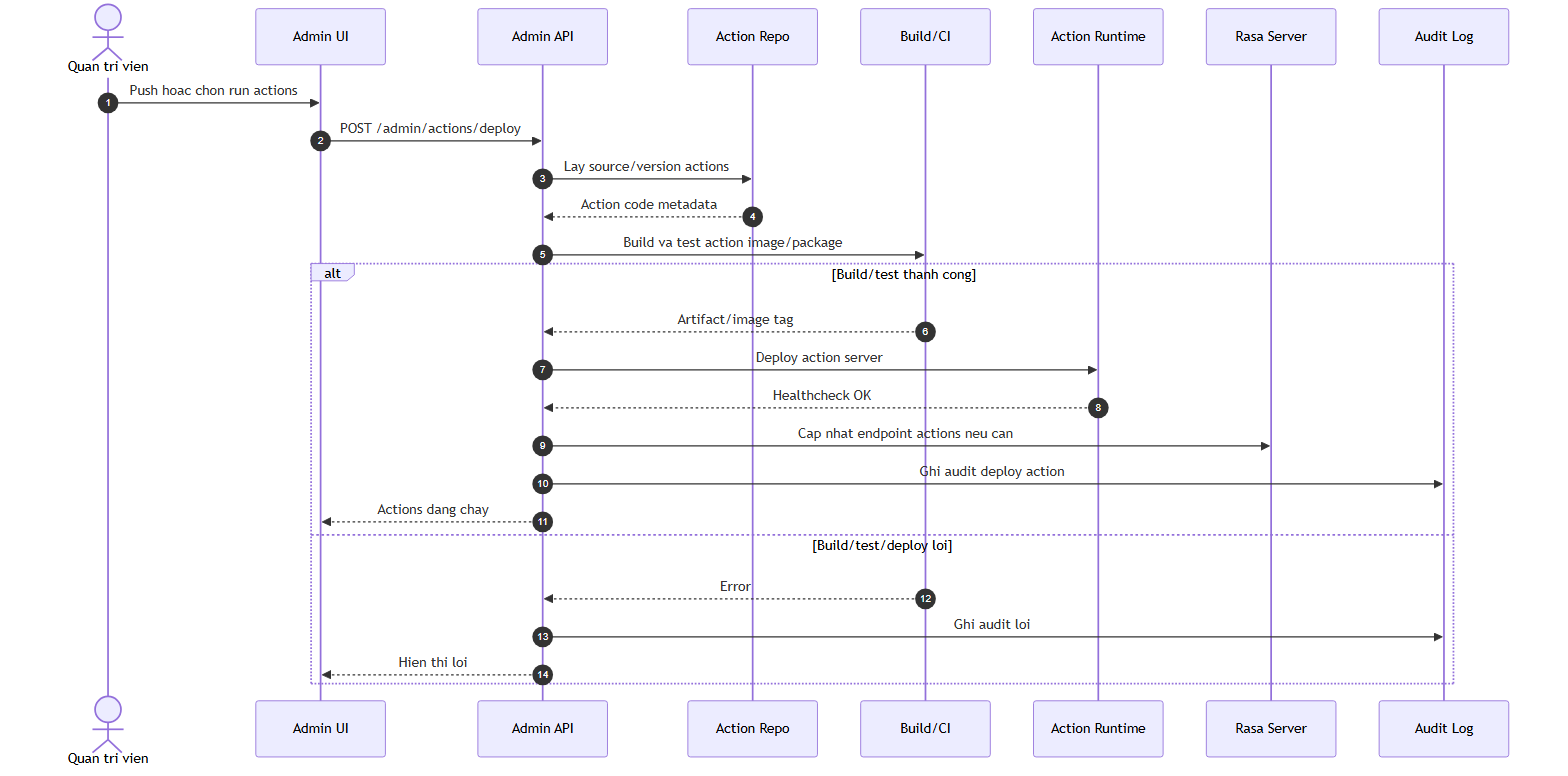
\includegraphics[width=\textwidth,height=0.78\textheight,keepaspectratio]{content/source/mermaid_sequence/seq_04.png}
    \caption{Sequence Diagram luồng push và chạy Action Server}
    \label{fig:seq-push-run-actions}
\end{figure}

\begin{figure}[H]
    \centering
    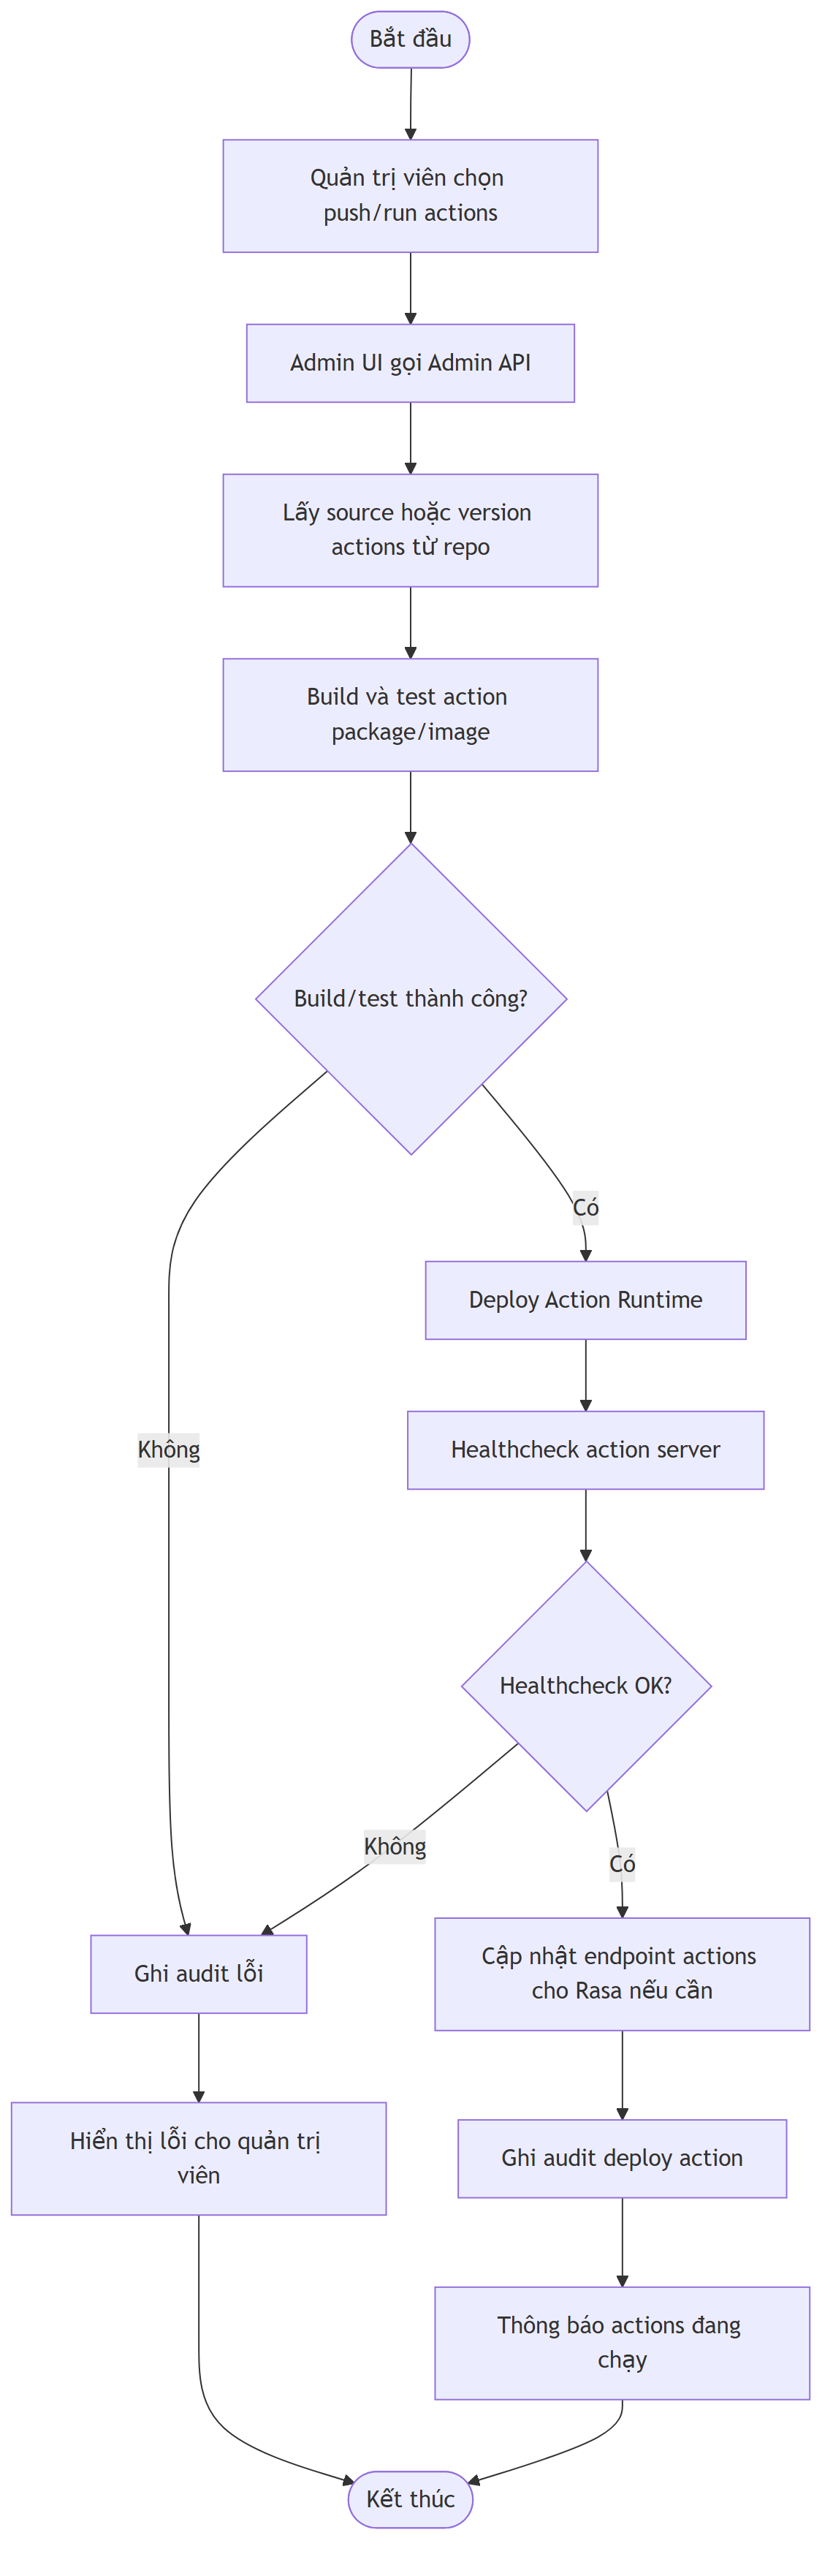
\includegraphics[width=\textwidth,height=0.78\textheight,keepaspectratio]{content/source/mermaid_activity/act_04.png}
    \caption{Activity Diagram luồng push và chạy Action Server}
    \label{fig:act-push-run-actions}
\end{figure}

\section{Thiết kế API Chatbot và huấn luyện mô hình}

Nhóm API chatbot phục vụ quá trình gửi câu hỏi, nhận phản hồi, kiểm tra trạng thái chatbot và vận hành các tiến trình liên quan đến Rasa.

\begin{longtable}{|p{3cm}|p{5cm}|p{7cm}|}
\hline
\textbf{Phương thức} & \textbf{Endpoint} & \textbf{Mô tả} \\
\hline
\texttt{POST} & \texttt{/v1/chatbot/chat/stream} & Gửi tin nhắn đến chatbot và nhận phản hồi dạng stream. \\
\hline
\texttt{GET} & \texttt{/v1/chatbot/\{id\}/models} & Lấy danh sách model của chatbot. \\
\hline
\texttt{GET} & \texttt{/v1/chatbot/\{id\}/health} & Kiểm tra trạng thái hoạt động của chatbot. \\
\hline
\texttt{POST} & \texttt{/v1/chatbot/\{id\}/run} & Chạy Rasa Server cho chatbot. \\
\hline
\texttt{POST} & \texttt{/v1/chatbot/\{id\}/run-actions} & Chạy Action Server cho chatbot. \\
\hline
\texttt{POST} & \texttt{/v1/chatbot/\{id\}/train} & Huấn luyện model chatbot. \\
\hline
\texttt{POST} & \texttt{/v1/chatbot/\{id\}/train-active} & Huấn luyện model từ các rule và story đang hoạt động. \\
\hline
\end{longtable}

\begin{figure}[H]
    \centering
    \includegraphics[width=\textwidth,height=0.78\textheight,keepaspectratio]{content/source/mermaid_sequence/IMG/Luồng upload run model.png}
    \caption{Sequence Diagram luồng upload và chạy model Rasa}
    \label{fig:seq-upload-run-model}
\end{figure}

\begin{figure}[H]
    \centering
    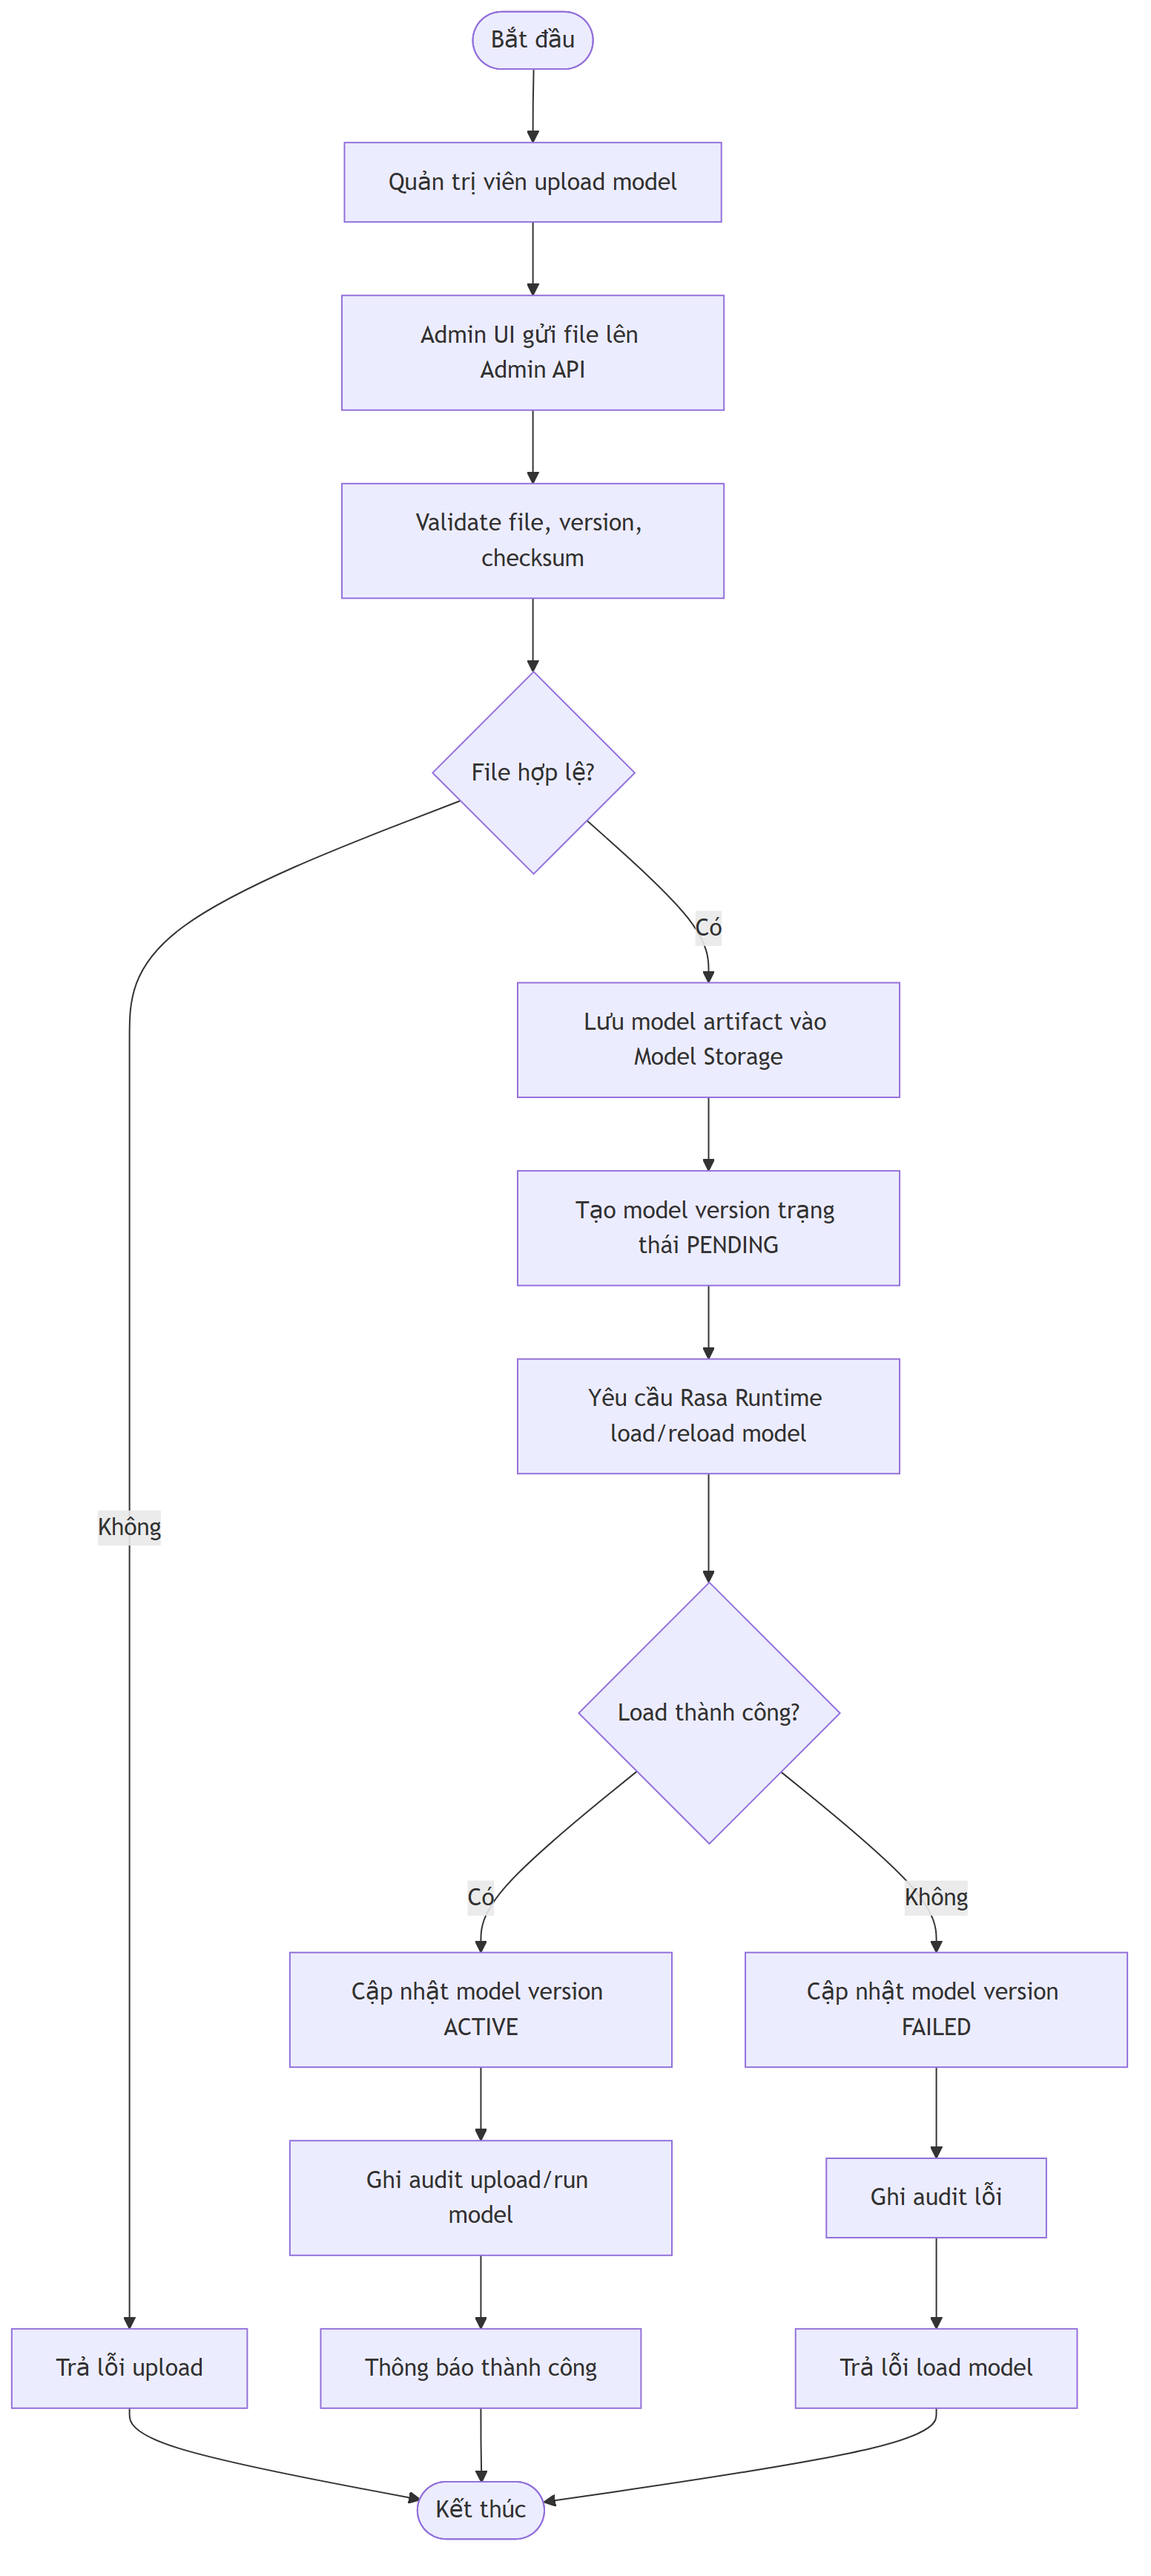
\includegraphics[width=\textwidth,height=0.78\textheight,keepaspectratio]{content/source/mermaid_activity/act_03.png}
    \caption{Activity Diagram luồng upload và chạy model Rasa}
    \label{fig:act-upload-run-model}
\end{figure}

\begin{figure}[H]
    \centering
    \includegraphics[width=\textwidth,height=0.78\textheight,keepaspectratio]{content/source/mermaid_sequence/IMG/Luồng active training data và train model.png}
    \caption{Sequence Diagram luồng active training data và train model}
    \label{fig:seq-active-training-data-train-model}
\end{figure}

\begin{figure}[H]
    \centering
    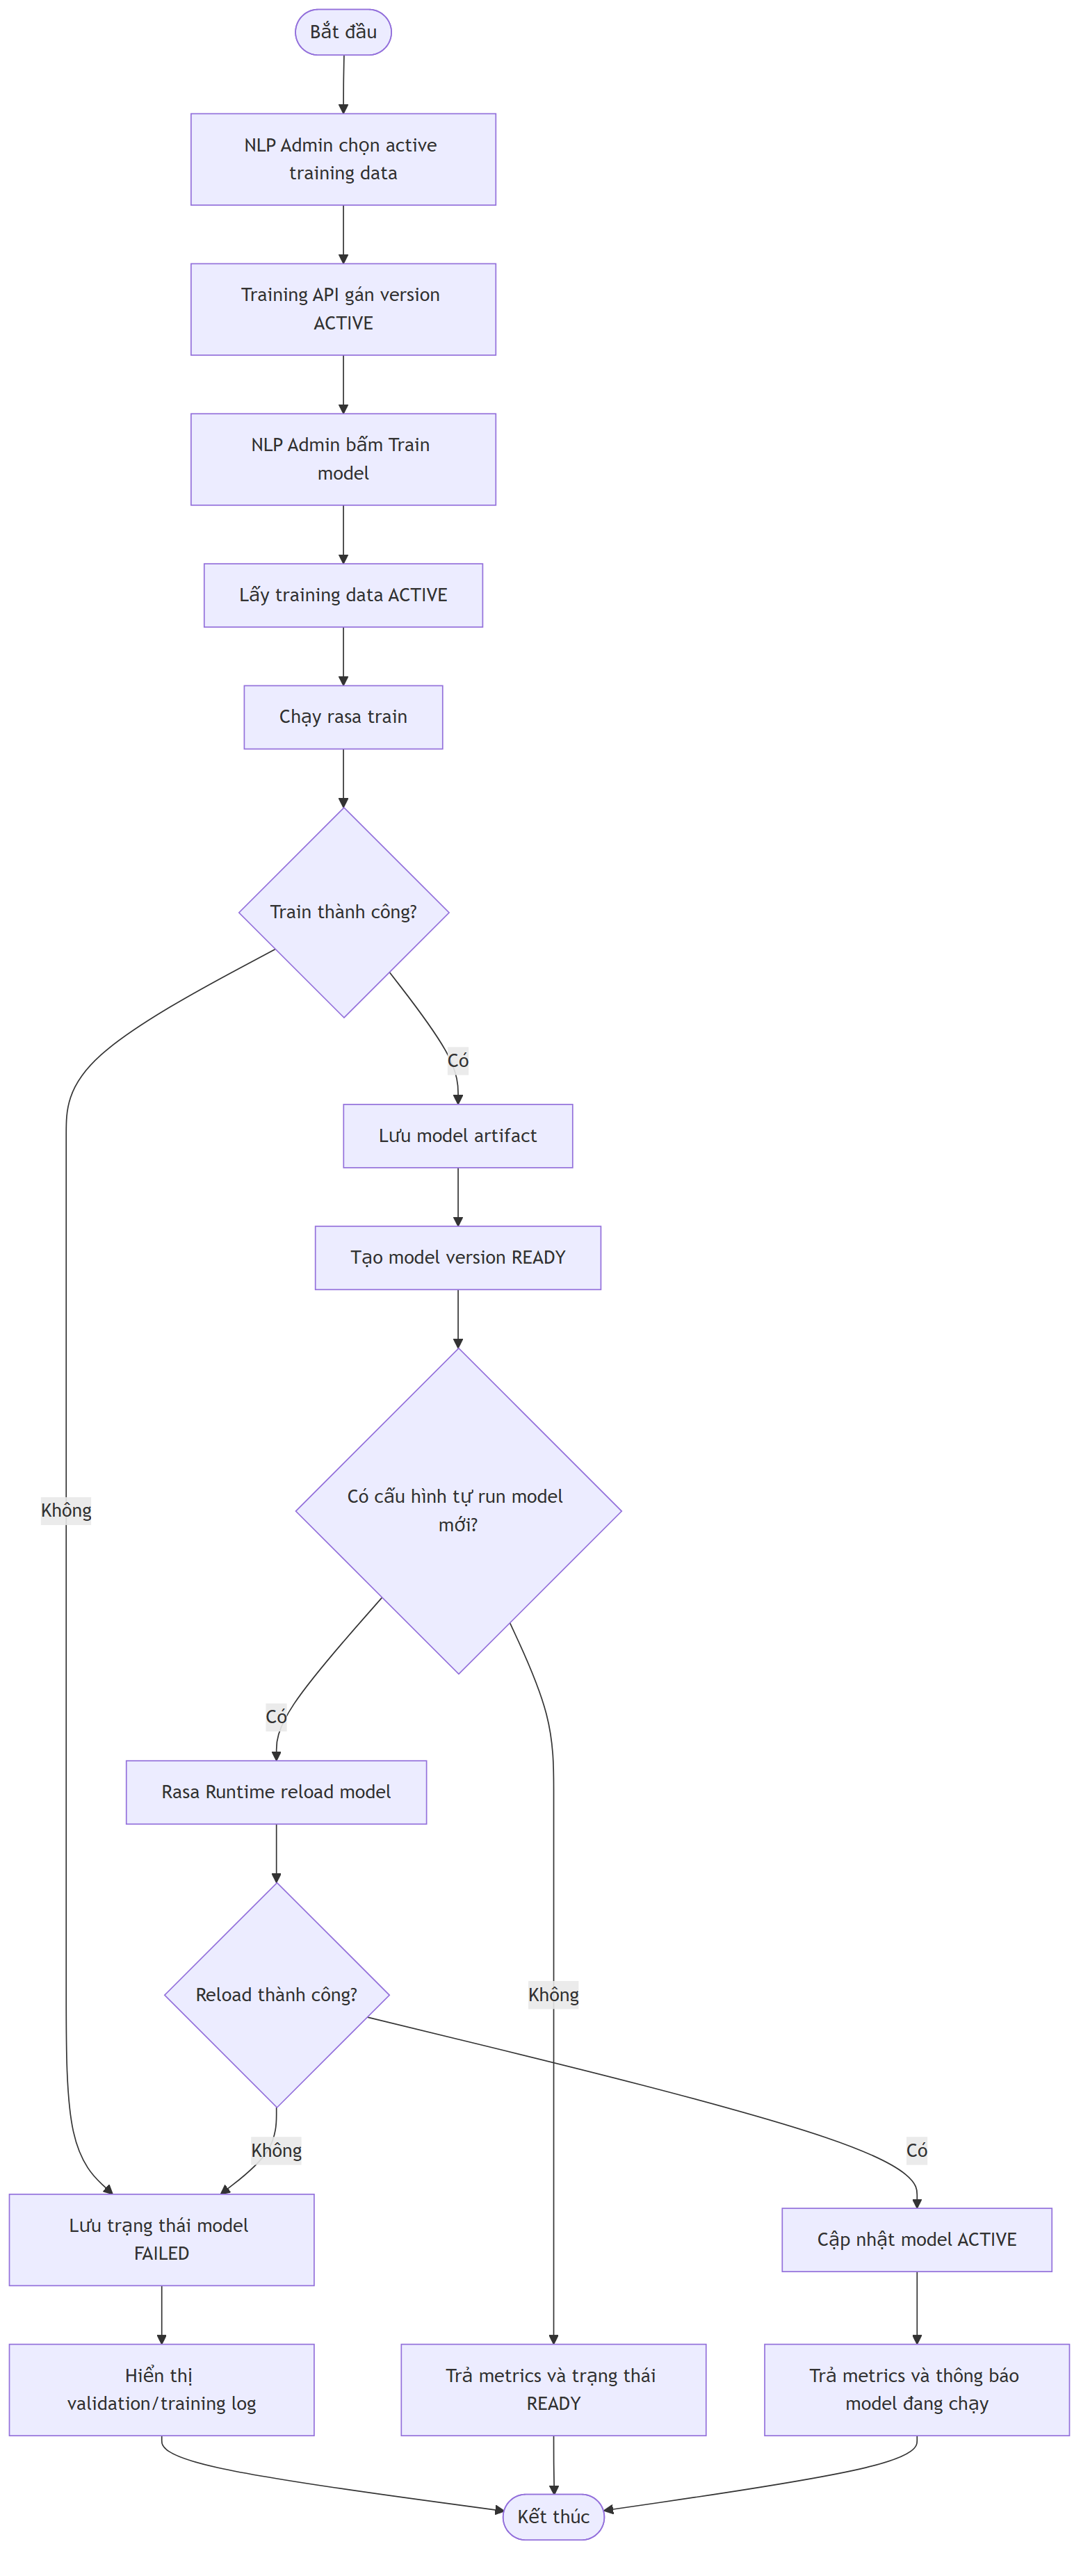
\includegraphics[width=\textwidth,height=0.78\textheight,keepaspectratio]{content/source/mermaid_activity/act_06.png}
    \caption{Activity Diagram luồng active training data và train model}
    \label{fig:act-active-training-data-train-model}
\end{figure}

Endpoint \texttt{/v1/chatbot/chat/stream} là API trung tâm trong quá trình tương tác với người dùng. Khi người dùng nhập câu hỏi, frontend gửi nội dung câu hỏi đến API này. Backend sau đó chuyển tiếp tin nhắn đến Rasa Server. Rasa phân tích intent, entity, trạng thái hội thoại và quyết định action cần thực hiện. Nếu cần dữ liệu nghiệp vụ, Rasa gọi Action Server. Nếu cần truy hồi tài liệu, Action Server gọi phân hệ RAG.

Ví dụ request gửi tin nhắn:

\begin{verbatim}
POST /api/v1/chatbot/chat/stream

{
  "message": "Ngành công nghệ thông tin lấy bao nhiêu điểm?",
  "senderId": "user-001",
  "conversationId": "conv-001"
}
\end{verbatim}

Ví dụ response dạng thông thường:

\begin{verbatim}
{
  "success": true,
  "data": {
    "answer": "Điểm chuẩn ngành Công nghệ thông tin năm gần nhất là ...",
    "source": "database",
    "intent": "ask_cutoff_score"
  }
}
\end{verbatim}

\section{Thiết kế API dữ liệu tuyển sinh cho Custom Actions}

Ngoài các API quản trị Rasa, hệ thống cần có nhóm API nghiệp vụ tuyển sinh để Action Server truy vấn dữ liệu có cấu trúc. Nhóm API này không nhất thiết được gọi trực tiếp bởi người dùng cuối mà chủ yếu phục vụ custom actions.

\begin{longtable}{|p{3cm}|p{5cm}|p{7cm}|}
\hline
\textbf{Phương thức} & \textbf{Endpoint đề xuất} & \textbf{Mô tả} \\
\hline
\texttt{GET} & \texttt{/v1/admissions/majors} & Lấy danh sách ngành học. \\
\hline
\texttt{GET} & \texttt{/v1/admissions/majors/\{id\}} & Lấy chi tiết ngành học. \\
\hline
\texttt{GET} & \texttt{/v1/admissions/majors/by-code/\{code\}} & Tra cứu ngành học theo mã ngành. \\
\hline
\texttt{GET} & \texttt{/v1/admissions/methods} & Lấy danh sách phương thức xét tuyển. \\
\hline
\texttt{GET} & \texttt{/v1/admissions/subject-combinations} & Lấy danh sách tổ hợp xét tuyển. \\
\hline
\texttt{GET} & \texttt{/v1/admissions/cutoff-scores} & Tra cứu điểm chuẩn theo ngành, năm hoặc phương thức xét tuyển. \\
\hline
\texttt{GET} & \texttt{/v1/admissions/tuitions} & Tra cứu học phí theo ngành và năm học. \\
\hline
\texttt{GET} & \texttt{/v1/admissions/faqs} & Lấy danh sách câu hỏi thường gặp. \\
\hline
\end{longtable}

Ví dụ khi người dùng hỏi: ``Học phí ngành An toàn thông tin là bao nhiêu?'', Rasa có thể nhận diện intent \texttt{ask\_tuition} và entity \texttt{major = An toàn thông tin}. Sau đó custom action gọi API:

\begin{verbatim}
GET /api/v1/admissions/tuitions?majorName=An%20toan%20thong%20tin&year=2025
\end{verbatim}

Kết quả trả về từ backend được Action Server định dạng lại thành câu trả lời tự nhiên trước khi gửi về Rasa. Cách thiết kế này giúp Rasa không phải lưu trực tiếp toàn bộ dữ liệu tuyển sinh trong file huấn luyện, đồng thời dữ liệu có thể được cập nhật thường xuyên từ giao diện quản trị.

\section{Thiết kế API cho phân hệ RAG}

API RAG được sử dụng khi câu hỏi của người dùng không thể trả lời tốt bằng rule, response tĩnh hoặc dữ liệu có cấu trúc. Đây thường là các câu hỏi dài, câu hỏi mở hoặc câu hỏi cần dựa vào tài liệu tuyển sinh.

Nhóm API RAG đề xuất gồm:

\begin{longtable}{|p{3cm}|p{5cm}|p{7cm}|}
\hline
\textbf{Phương thức} & \textbf{Endpoint đề xuất} & \textbf{Mô tả} \\
\hline
\texttt{POST} & \texttt{/v1/rag/query} & Gửi câu hỏi đến phân hệ RAG và nhận câu trả lời kèm nguồn. \\
\hline
\texttt{POST} & \texttt{/v1/rag/documents} & Thêm tài liệu mới vào kho tri thức. \\
\hline
\texttt{GET} & \texttt{/v1/rag/documents} & Lấy danh sách tài liệu đã ingest. \\
\hline
\texttt{GET} & \texttt{/v1/rag/documents/\{id\}} & Xem chi tiết tài liệu. \\
\hline
\texttt{POST} & \texttt{/v1/rag/documents/\{id\}/ingest} & Thực hiện ingest tài liệu vào kho tri thức. \\
\hline
\texttt{POST} & \texttt{/v1/rag/documents/\{id\}/retry} & Xử lý lại tài liệu bị lỗi. \\
\hline
\texttt{DELETE} & \texttt{/v1/rag/documents/\{id\}} & Xóa tài liệu khỏi kho tri thức. \\
\hline
\texttt{GET} & \texttt{/v1/rag/health} & Kiểm tra trạng thái các thành phần RAG. \\
\hline
\end{longtable}

Request truy vấn RAG có thể có dạng:

\begin{verbatim}
POST /api/v1/rag/query

{
  "question": "Điều kiện xét tuyển thẳng của trường là gì?",
  "conversationId": "conv-001",
  "topK": 5,
  "filters": {
    "year": 2025,
    "documentType": "admission_policy"
  }
}
\end{verbatim}

Response RAG cần trả về câu trả lời và nguồn tham chiếu:

\begin{verbatim}
{
  "success": true,
  "data": {
    "answer": "Theo đề án tuyển sinh, điều kiện xét tuyển thẳng gồm ...",
    "sources": [
      {
        "documentName": "De an tuyen sinh 2025.pdf",
        "chunkId": "chunk-001",
        "page": 12,
        "score": 0.87
      }
    ]
  }
}
\end{verbatim}

Thiết kế response có nguồn tham chiếu giúp tăng độ tin cậy của câu trả lời và hỗ trợ người dùng kiểm chứng thông tin. Đồng thời, quản trị viên có thể dựa vào thông tin \texttt{chunkId}, \texttt{documentName} và \texttt{score} để đánh giá chất lượng truy hồi.

\section{Luồng tích hợp API giữa Frontend, Backend, Rasa và RAG}

Trong hệ thống, frontend không gọi trực tiếp đến Rasa Server hoặc RAG Service mà gửi yêu cầu thông qua backend. Backend đóng vai trò điều phối, xác thực, ghi log hội thoại và chuyển tiếp request đến thành phần phù hợp.

Luồng xử lý câu hỏi thông thường như sau:

\begin{enumerate}
    \item Người dùng nhập câu hỏi trên giao diện chat.
    \item Frontend gọi API \texttt{POST /v1/chatbot/chat/stream}.
    \item Backend ghi nhận tin nhắn và gửi câu hỏi đến Rasa Server.
    \item Rasa Server nhận diện intent, entity và quyết định action.
    \item Nếu action là phản hồi tĩnh, Rasa trả lời bằng response đã cấu hình.
    \item Nếu action cần dữ liệu tuyển sinh, Action Server gọi API dữ liệu tuyển sinh của backend.
    \item Nếu action cần tài liệu, Action Server gọi API \texttt{/v1/rag/query}.
    \item Backend trả kết quả về frontend và lưu lịch sử hội thoại.
\end{enumerate}

Với thiết kế này, mỗi thành phần trong hệ thống có nhiệm vụ rõ ràng. Frontend chỉ phụ trách giao diện và trải nghiệm người dùng. Backend phụ trách xác thực, điều phối và quản lý dữ liệu. Rasa phụ trách hiểu ý định và quản lý hội thoại. Action Server xử lý nghiệp vụ động. RAG phụ trách truy hồi tài liệu và sinh câu trả lời dựa trên kho tri thức.

\begin{figure}[H]
    \centering
    \includegraphics[width=\textwidth,height=0.78\textheight,keepaspectratio]{content/source/mermaid_sequence/IMG/Luồng lưu lịch sử hội thoại.png}
    \caption{Sequence Diagram luồng lưu lịch sử hội thoại}
    \label{fig:seq-conversation-history}
\end{figure}

\section{Kết luận chương}

Chương này đã trình bày thiết kế API cho hệ thống chatbot tư vấn tuyển sinh. Các API được chia thành các nhóm chính gồm API xác thực, API quản lý dữ liệu Rasa, API chatbot, API huấn luyện mô hình, API dữ liệu tuyển sinh và API RAG. Thiết kế này giúp hệ thống có cấu trúc rõ ràng, dễ mở rộng và phù hợp với mô hình kết hợp giữa Rasa và RAG.

Thông qua lớp API, hệ thống có thể quản lý dữ liệu huấn luyện chatbot, vận hành Rasa, gọi custom actions, truy xuất dữ liệu tuyển sinh và khai thác kho tri thức. Đây là nền tảng quan trọng để triển khai các chức năng hỏi đáp tự động, quản trị nội dung và cải thiện chất lượng tư vấn tuyển sinh trong quá trình vận hành.



\chapter{PHÂN TÍCH VÀ THIẾT KẾ PHÂN HỆ QUẢN TRỊ}

\section{Vai trò của phân hệ quản trị}

Phân hệ quản trị là thành phần quan trọng trong hệ thống KMA Chatbot tuyển sinh, có nhiệm vụ hỗ trợ người quản trị kiểm soát dữ liệu, tài liệu, người dùng, quyền truy cập, thống kê vận hành và kho tri thức phục vụ hỏi đáp. Nếu giao diện hội thoại là nơi người dùng cuối đặt câu hỏi và nhận câu trả lời, thì phân hệ quản trị là nơi duy trì dữ liệu nền, kiểm soát trạng thái xử lý tài liệu, theo dõi chất lượng vận hành và đảm bảo hệ thống hoạt động đúng phạm vi được cấu hình.

Từ giao diện hệ thống đã quan sát, phân hệ quản trị bao gồm các nhóm chức năng chính: quản lý tài liệu và biểu mẫu, quản lý tài liệu ngữ cảnh RAG, báo cáo thống kê, quản lý chatbot theo ngữ cảnh đang chọn, quản lý vai trò, quản lý quyền và quản lý người dùng. Các nhóm chức năng này cho thấy hệ thống không chỉ dừng lại ở một chatbot hỏi đáp đơn giản, mà đã được mở rộng thành một nền tảng quản trị tri thức và vận hành chatbot phục vụ tư vấn tuyển sinh.

Trong bài toán tuyển sinh, dữ liệu thường xuyên thay đổi theo từng năm như phương thức xét tuyển, điểm chuẩn, chương trình đào tạo, biểu mẫu, quy chế, lịch tuyển sinh và các thông báo mới. Vì vậy, phân hệ quản trị đóng vai trò cầu nối giữa người quản trị nội dung và các thành phần kỹ thuật phía sau như Backend API, Rasa, RAG service, cơ sở dữ liệu, kho tài liệu và vector database.

Các mục tiêu chính của phân hệ quản trị gồm:

\begin{itemize}
    \item Quản lý tài liệu, biểu mẫu phục vụ sinh viên, thí sinh và cán bộ.
    \item Quản lý tài liệu ngữ cảnh được đưa vào kho tri thức RAG.
    \item Theo dõi trạng thái xử lý tài liệu như processed, pending, failed.
    \item Hỗ trợ upload, scan, retry pipeline và làm mới dữ liệu tài liệu.
    \item Quản lý chatbot theo ngữ cảnh được chọn.
    \item Theo dõi các báo cáo thống kê về người dùng, hội thoại, chatbot và tài liệu.
    \item Quản lý vai trò, quyền và tài khoản người dùng theo mô hình RBAC.
    \item Đảm bảo chỉ người dùng có quyền phù hợp mới được truy cập các chức năng quản trị.
\end{itemize}

Như vậy, phân hệ quản trị vừa có vai trò nghiệp vụ, vừa có vai trò kỹ thuật. Về mặt nghiệp vụ, phân hệ giúp cập nhật dữ liệu và tài liệu tư vấn. Về mặt kỹ thuật, phân hệ giúp kiểm soát trạng thái xử lý dữ liệu, phân quyền truy cập và theo dõi hiệu quả vận hành của chatbot.

\section{Tổng quan giao diện quản trị}

Giao diện quản trị được tổ chức theo dạng sidebar, cho phép người dùng truy cập nhanh đến các nhóm chức năng chính. Các route đã quan sát gồm \texttt{/docs}, \texttt{/context-docs}, \texttt{/statistics/users}, \texttt{/statistics/conversations}, \texttt{/statistics/chatbots}, \texttt{/statistics/documents}, \texttt{/roles}, \texttt{/permissions} và \texttt{/users}. Ngoài ra, khu vực giao diện còn hiển thị trường chọn chatbot với giá trị quan sát được là \textit{Chatbot tuyen sinh}.

Việc có trường chọn chatbot trên nhiều màn hình quản trị cho thấy hệ thống được thiết kế theo hướng có thể vận hành theo ngữ cảnh chatbot. Khi người quản trị chọn một chatbot cụ thể, các dữ liệu như tài liệu, ngữ cảnh RAG, thống kê và phân quyền có thể được khoanh vùng theo chatbot đó. Cách thiết kế này phù hợp với hệ thống có khả năng mở rộng để quản lý nhiều chatbot trong tương lai, ví dụ chatbot tuyển sinh, chatbot hỗ trợ sinh viên hoặc chatbot tư vấn học vụ.

Các nhóm màn hình chính trong phân hệ quản trị gồm:

\begin{itemize}
    \item \textbf{Documents \& Forms}: quản lý tài liệu và biểu mẫu.
    \item \textbf{Context Documents}: quản lý tài liệu ngữ cảnh cho RAG.
    \item \textbf{Statistics}: thống kê người dùng, hội thoại, chatbot và tài liệu.
    \item \textbf{RBAC}: quản lý vai trò và quyền.
    \item \textbf{Users Management}: quản lý tài khoản người dùng.
\end{itemize}

\begin{figure}[H]
    \centering
    % \includegraphics[width=0.9\textwidth]{images/admin-overview.png}
    \caption{Tổng quan giao diện phân hệ quản trị}
    \label{fig:admin-overview}
\end{figure}

\section{Thiết kế dashboard và nhóm báo cáo quản trị}

Dashboard và nhóm báo cáo quản trị có nhiệm vụ cung cấp góc nhìn tổng quan về tình trạng hoạt động của hệ thống. Trong giao diện đã phân tích, hệ thống có các màn hình thống kê chính gồm User Report, Conversation Report, Chatbot Report và Document Report. Riêng route \texttt{/statistics/nlp} trong phiên quan sát hiện tại chưa tải được đầy đủ, do đó phần thiết kế chỉ mô tả theo hướng chức năng cần có và không khẳng định số liệu NLP cụ thể.

\subsection{Báo cáo người dùng}

Báo cáo người dùng giúp người quản trị theo dõi số lượng tài khoản và trạng thái hoạt động của người dùng trong hệ thống. Các chỉ số cần hiển thị gồm tổng số người dùng, số người dùng đang hoạt động, số người dùng bị khóa, số người dùng chờ duyệt và số người dùng mới trong một khoảng thời gian.

Báo cáo này có ý nghĩa quan trọng trong vận hành vì nó giúp Admin kiểm soát quy mô người dùng, phát hiện tài khoản bất thường và đánh giá mức độ sử dụng hệ thống.

\subsection{Báo cáo hội thoại}

Báo cáo hội thoại phục vụ theo dõi hoạt động hỏi đáp giữa người dùng và chatbot. Màn hình Conversation Report đã quan sát có các thẻ thống kê và biểu đồ xu hướng hội thoại. Về mặt thiết kế, báo cáo hội thoại cần hiển thị các thông tin như tổng số hội thoại, số lượng tin nhắn trung bình, người dùng đang hoạt động và xu hướng hội thoại theo thời gian.

Các chỉ số này giúp người quản trị biết thời điểm hệ thống được sử dụng nhiều, nhóm câu hỏi nào phát sinh thường xuyên và mức độ tương tác của người dùng với chatbot.

\begin{figure}[H]
    \centering
    \includegraphics[width=\textwidth,height=0.78\textheight,keepaspectratio]{content/source/mermaid_sequence/IMG/Luồng lưu lịch sử hội thoại.png}
    \caption{Sequence Diagram luồng lưu và tra cứu lịch sử hội thoại}
    \label{fig:seq-admin-conversation-history}
\end{figure}

\begin{figure}[H]
    \centering
    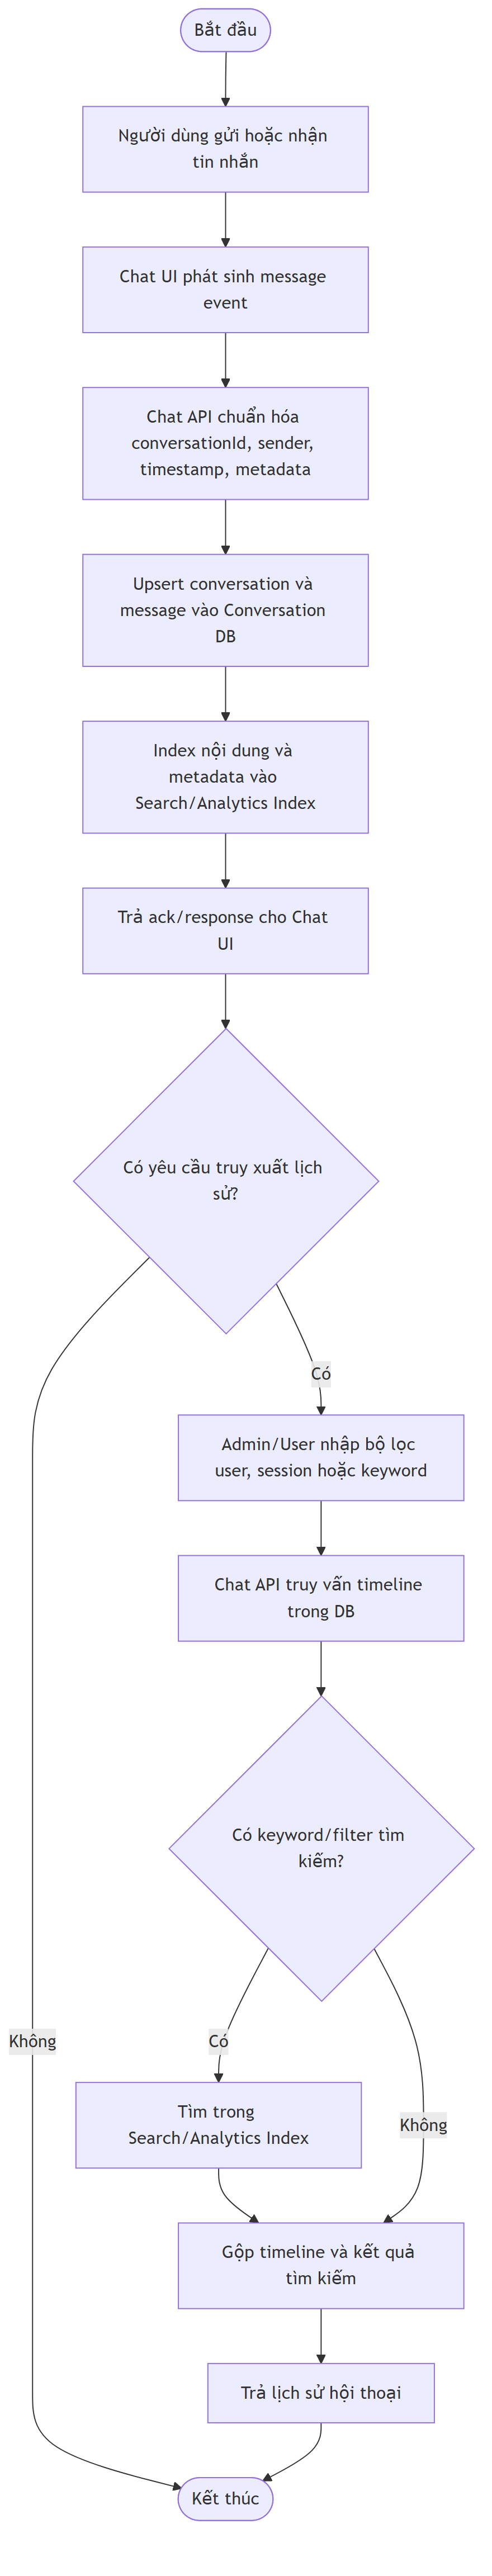
\includegraphics[width=\textwidth,height=0.78\textheight,keepaspectratio]{content/source/mermaid_activity/act_11.png}
    \caption{Activity Diagram luồng lưu và tra cứu lịch sử hội thoại}
    \label{fig:act-admin-conversation-history}
\end{figure}

\subsection{Báo cáo chatbot}

Báo cáo chatbot tập trung vào các chatbot đang được quản lý trong hệ thống. Màn hình Chatbot Report đã xác minh có nhóm thông tin về tổng số chatbot, tổng số người dùng và số lượng intent đang hoạt động. Điều này cho thấy backend đã có nhóm thống kê riêng cho đối tượng chatbot.

Trong thiết kế, báo cáo chatbot cần cung cấp các thông tin:

\begin{itemize}
    \item Tổng số chatbot đang có trong hệ thống.
    \item Chatbot đang được chọn làm ngữ cảnh quản trị.
    \item Số người dùng liên quan đến chatbot.
    \item Số intent hoặc nhóm nghiệp vụ mà chatbot hỗ trợ.
    \item Trạng thái hoạt động của chatbot.
\end{itemize}

Tuy nhiên, trong phạm vi dữ liệu UI hiện có, chưa xác minh được màn hình tạo, sửa, xóa chatbot riêng biệt. Vì vậy, chương này chỉ mô tả quản lý chatbot ở mức chọn ngữ cảnh và theo dõi thống kê, không khẳng định đầy đủ chức năng CRUD chatbot.

\subsection{Báo cáo tài liệu}

Báo cáo tài liệu giúp theo dõi tình trạng kho tài liệu của hệ thống. Màn hình Document Report đã quan sát có các chỉ số như tổng số tài liệu, số tài liệu public, số tài liệu private và tổng dung lượng file. Ngoài ra, màn hình còn có các biểu đồ phân bố theo loại file, dung lượng và trạng thái public/private.

Báo cáo tài liệu giúp Admin đánh giá quy mô kho tài liệu, loại file đang được sử dụng nhiều và mức độ công khai của tài liệu. Đây là cơ sở để kiểm soát chất lượng dữ liệu đầu vào cho hệ thống hỏi đáp và kho tri thức.

\begin{figure}[H]
    \centering
    % \includegraphics[width=0.9\textwidth]{images/statistics-document-report.png}
    \caption{Màn hình báo cáo tài liệu}
    \label{fig:statistics-document-report}
\end{figure}

\section{Phân hệ quản lý chatbot}

Phân hệ quản lý chatbot trong giao diện hiện tại được thể hiện thông qua trường chọn chatbot trên nhiều màn hình quản trị như tài liệu, tài liệu ngữ cảnh, thống kê, vai trò, quyền và người dùng. Giá trị quan sát được là \textit{Chatbot tuyen sinh}. Điều này cho thấy hệ thống có khả năng khoanh vùng dữ liệu theo chatbot đang được chọn.

\subsection{Chọn ngữ cảnh chatbot}

Khi người quản trị chọn một chatbot, các thao tác tiếp theo trong khu vực quản trị có thể được hiểu là đang áp dụng cho chatbot đó. Ví dụ, khi chọn \textit{Chatbot tuyen sinh}, danh sách tài liệu, tài liệu ngữ cảnh, thống kê và quyền truy cập có thể được lọc theo phạm vi chatbot tuyển sinh.

Thiết kế này có ưu điểm là giúp hệ thống mở rộng tốt hơn. Trong tương lai, nếu nhà trường triển khai thêm nhiều chatbot khác nhau, ví dụ chatbot học vụ, chatbot thư viện hoặc chatbot hỗ trợ kỹ thuật, Admin có thể chuyển đổi ngữ cảnh quản trị mà không cần xây dựng một hệ thống riêng cho từng chatbot.

\subsection{Thống kê theo chatbot}

Route \texttt{/statistics/chatbots} và quyền \texttt{GET /api/v1/statistic/chatbots} cho thấy hệ thống đã có nhóm thống kê dành riêng cho chatbot. Điều này giúp Admin theo dõi hiệu quả hoạt động của từng chatbot thay vì chỉ xem thống kê tổng thể toàn hệ thống.

Các chỉ số nên được quản lý theo chatbot gồm:

\begin{itemize}
    \item Số lượng người dùng tương tác với chatbot.
    \item Số lượng hội thoại phát sinh từ chatbot.
    \item Số intent đang hoạt động.
    \item Số tài liệu hoặc tài liệu ngữ cảnh được gắn với chatbot.
    \item Trạng thái hoạt động của chatbot.
\end{itemize}

\subsection{Giới hạn phạm vi đã xác minh}

Trong phiên phân tích UI hiện tại, chưa ghi nhận được màn hình tạo, sửa, xóa chatbot riêng biệt. Vì vậy, chức năng quản lý chatbot trong chương này được mô tả theo phạm vi đã xác minh gồm chọn ngữ cảnh chatbot và xem thống kê chatbot. Các chức năng CRUD chatbot nếu có sẽ cần được kiểm chứng thêm trong quá trình phát triển hoặc kiểm thử hệ thống.

\section{Phân hệ quản lý tài liệu và biểu mẫu}

Phân hệ quản lý tài liệu và biểu mẫu được truy cập thông qua route \texttt{/docs}. Màn hình này hiển thị danh sách tài liệu biểu mẫu với các cột như Document Name, Description, Tags, File Type, File Size, Created At và Actions. Các tài liệu quan sát được gồm nhiều loại biểu mẫu như đơn hủy học phần, giấy giới thiệu thực tập, đơn xin đăng ký đồ án lần 2, đơn xin cấp lại thẻ bảo hiểm y tế, đơn xin bảo lưu điểm thi lại, đơn xin phúc khảo bài thi, đơn xin hoãn thi, thanh toán ra trường và đơn xin thôi học.

\subsection{Mục đích của quản lý tài liệu và biểu mẫu}

Chức năng này giúp nhà trường tập trung quản lý các biểu mẫu thường dùng để người dùng có thể tra cứu, tải xuống hoặc được chatbot hướng dẫn sử dụng khi cần. Trong bối cảnh tuyển sinh và đào tạo, biểu mẫu là nhóm tài liệu có tần suất sử dụng cao, đặc biệt đối với sinh viên, thí sinh và cán bộ xử lý hồ sơ.

Việc đưa biểu mẫu vào hệ thống quản trị giúp giảm thao tác thủ công, hạn chế tình trạng sử dụng biểu mẫu cũ và tạo nền tảng để chatbot có thể trả lời các câu hỏi như: ``Em muốn xin hoãn thi thì dùng mẫu nào?'', ``Mẫu đơn xin phúc khảo ở đâu?'' hoặc ``Có giấy giới thiệu thực tập không?''.

\subsection{Thông tin tài liệu cần quản lý}

Mỗi tài liệu hoặc biểu mẫu cần lưu các thông tin chính sau:

\begin{itemize}
    \item Tên tài liệu.
    \item Mô tả tài liệu.
    \item Danh sách tag.
    \item Loại file.
    \item Dung lượng file.
    \item Thời điểm tạo.
    \item Trạng thái public/private nếu có.
    \item Các thao tác quản trị như xem, sửa, tải xuống, khôi phục hoặc xóa mềm.
\end{itemize}

Các trường này phù hợp với các cột đã quan sát trên màn hình \texttt{/docs}. Trong đó, tag giúp phân loại tài liệu theo nhóm nghiệp vụ, loại file giúp người dùng biết định dạng tài liệu và dung lượng file giúp kiểm soát lưu trữ.

\subsection{Tìm kiếm, lọc và thao tác tài liệu}

Màn hình quản lý tài liệu cần hỗ trợ tìm kiếm theo tên tài liệu, mô tả và tag. Ngoài ra, hệ thống cần cho phép lọc theo loại file, trạng thái public/private hoặc thời gian tạo. Đối với danh sách tài liệu lớn, cần có phân trang để đảm bảo giao diện dễ sử dụng.

Các thao tác cơ bản gồm:

\begin{itemize}
    \item Thêm tài liệu mới.
    \item Cập nhật thông tin mô tả hoặc tag.
    \item Tải xuống tài liệu.
    \item Xóa mềm tài liệu.
    \item Khôi phục tài liệu đã xóa mềm.
\end{itemize}

Việc xuất hiện quyền \texttt{POST /api/v1/documents/:id/restore} và \texttt{DELETE /api/v1/documents/:id/soft} cho thấy hệ thống đã tính đến cơ chế khôi phục và xóa mềm tài liệu. Đây là thiết kế phù hợp vì tài liệu quản trị không nên bị xóa vĩnh viễn ngay lập tức, nhằm đảm bảo khả năng truy vết và phục hồi khi thao tác nhầm.

\begin{figure}[H]
    \centering
    % \includegraphics[width=0.9\textwidth]{images/docs.png}
    \caption{Màn hình quản lý tài liệu và biểu mẫu}
    \label{fig:docs-management}
\end{figure}

\section{Phân hệ quản lý tài liệu ngữ cảnh RAG}

Phân hệ quản lý tài liệu ngữ cảnh RAG được truy cập thông qua route \texttt{/context-docs}. Đây là một trong những chức năng quan trọng nhất của hệ thống vì nó quyết định nguồn tri thức mà RAG sử dụng để truy hồi và sinh câu trả lời.

\subsection{Mục đích của tài liệu ngữ cảnh}

Tài liệu ngữ cảnh là các tài liệu được đưa vào pipeline xử lý của RAG. Sau khi upload hoặc scan, tài liệu được trích xuất nội dung, chia thành chunks, sinh embedding và lưu vào các lớp lưu trữ phục vụ truy hồi. Khi người dùng đặt câu hỏi, RAG sẽ tìm các chunks liên quan và sử dụng chúng làm ngữ cảnh để sinh câu trả lời.

Trong hệ thống KMA Chatbot tuyển sinh, các tài liệu ngữ cảnh đã quan sát gồm quy chế tuyển sinh, điểm chuẩn, chương trình đào tạo, quy định đào tạo, kế hoạch hoạt động và các tài liệu liên quan đến học viện. Đây là nguồn tri thức quan trọng để chatbot trả lời các câu hỏi có nội dung dài, phức tạp hoặc cần bám sát tài liệu gốc.

\subsection{Các thao tác trên màn hình Context Documents}

Màn hình \texttt{/context-docs} hiển thị các nút chức năng như Scan New Docs, Retry Pipeline, Pipeline, Refresh, Clear All, Upload Documents, bộ lọc trạng thái và bảng danh sách tài liệu. Các thao tác này thể hiện rõ vai trò vận hành của phân hệ RAG.

Ý nghĩa của các thao tác chính như sau:

\begin{itemize}
    \item \textbf{Scan New Docs}: quét tài liệu mới từ thư mục hoặc nguồn đầu vào đã cấu hình.
    \item \textbf{Upload Documents}: tải tài liệu mới lên hệ thống.
    \item \textbf{Retry Pipeline}: xử lý lại các tài liệu bị lỗi.
    \item \textbf{Pipeline}: xem hoặc kiểm tra trạng thái pipeline xử lý tài liệu.
    \item \textbf{Refresh}: làm mới danh sách tài liệu và trạng thái xử lý.
    \item \textbf{Clear All}: xóa hoặc làm sạch danh sách tài liệu trong phạm vi được phép.
    \item \textbf{Bộ lọc trạng thái}: lọc tài liệu theo trạng thái như processed, pending hoặc failed.
\end{itemize}

Việc có nút Retry Pipeline và trạng thái Failed cho thấy hệ thống đã tính đến các lỗi có thể xảy ra trong quá trình ingest, OCR, trích xuất văn bản, chia chunks hoặc sinh embedding. Đây là yêu cầu quan trọng đối với hệ thống RAG vận hành thực tế.

\subsection{Trạng thái xử lý tài liệu}

Mỗi tài liệu ngữ cảnh cần có trạng thái xử lý rõ ràng để người quản trị biết tài liệu đã sẵn sàng được sử dụng hay chưa. Các trạng thái chính gồm:

\begin{itemize}
    \item \textbf{Processed}: tài liệu đã được xử lý thành công và có thể phục vụ truy hồi.
    \item \textbf{Pending}: tài liệu đang chờ xử lý.
    \item \textbf{Processing}: tài liệu đang được pipeline xử lý.
    \item \textbf{Failed}: tài liệu xử lý lỗi, cần kiểm tra hoặc retry.
\end{itemize}

Ngoài trạng thái, bảng tài liệu cần hiển thị số chunks, tóm tắt nội dung và thời điểm cập nhật. Đây là các thông tin giúp Admin đánh giá tài liệu đã được ingest đúng hay chưa.

\subsection{Luồng xử lý tài liệu RAG}

Luồng xử lý tài liệu RAG trong phân hệ quản trị có thể mô tả như sau:

\begin{enumerate}
    \item Admin hoặc Editor upload tài liệu mới.
    \item Hệ thống kiểm tra định dạng file và dung lượng.
    \item Tài liệu được đưa vào hàng đợi xử lý.
    \item Pipeline trích xuất văn bản từ file.
    \item Nội dung được làm sạch và chuẩn hóa.
    \item Văn bản được chia thành các chunks.
    \item Hệ thống sinh embedding cho từng chunk.
    \item Chunks và metadata được lưu vào kho dữ liệu tương ứng.
    \item Trạng thái tài liệu được cập nhật trên giao diện quản trị.
\end{enumerate}

\begin{figure}[H]
    \centering
    % \includegraphics[width=0.9\textwidth]{images/context-docs.png}
    \caption{Màn hình quản lý tài liệu ngữ cảnh RAG}
    \label{fig:context-docs}
\end{figure}

\subsection{Thiết kế kiểm soát lỗi pipeline}

Do pipeline xử lý tài liệu có nhiều bước, hệ thống cần thiết kế cơ chế kiểm soát lỗi rõ ràng. Khi một tài liệu bị lỗi, hệ thống cần lưu nguyên nhân lỗi, thời điểm lỗi và bước xử lý xảy ra lỗi. Người quản trị có thể nhấn Retry Pipeline để xử lý lại tài liệu sau khi nguyên nhân được khắc phục.

Các lỗi có thể gặp gồm:

\begin{itemize}
    \item File không đúng định dạng.
    \item File quá lớn hoặc bị hỏng.
    \item Không trích xuất được văn bản từ PDF.
    \item Lỗi encoding tiếng Việt.
    \item Lá»—i chia chunks.
    \item Lỗi gọi mô hình embedding.
    \item Lỗi ghi dữ liệu vào vector database.
\end{itemize}

Thiết kế này giúp phân hệ quản trị không chỉ là nơi upload tài liệu mà còn là nơi vận hành, giám sát và khắc phục sự cố của toàn bộ pipeline RAG.

\section{Phân hệ báo cáo thống kê}

Phân hệ báo cáo thống kê được tổ chức trong nhóm route \texttt{/statistics/*}. Các màn hình đã xác minh gồm User Report, Conversation Report, Chatbot Report và Document Report. Mục tiêu của phân hệ này là cung cấp số liệu phục vụ quản trị, đánh giá mức độ sử dụng và theo dõi tình trạng dữ liệu.

\subsection{Thống kê người dùng}

Thống kê người dùng cho phép Admin theo dõi số lượng người dùng trong hệ thống, tình trạng tài khoản và mức độ hoạt động. Các chỉ số cần có gồm:

\begin{itemize}
    \item Tổng số người dùng.
    \item Số người dùng đang hoạt động.
    \item Số người dùng chờ duyệt.
    \item Số người dùng bị khóa hoặc bị cấm.
    \item Số người dùng mới theo thời gian.
\end{itemize}

Nhóm thống kê này giúp Admin phát hiện bất thường trong hệ thống tài khoản, đồng thời hỗ trợ đánh giá quy mô người dùng thực tế.

\subsection{Thống kê hội thoại}

Thống kê hội thoại giúp theo dõi hoạt động tương tác giữa người dùng và chatbot. Các chỉ số cần có gồm:

\begin{itemize}
    \item Tổng số hội thoại.
    \item Tổng số tin nhắn.
    \item Số tin nhắn trung bình trên mỗi hội thoại.
    \item Số người dùng đang hội thoại.
    \item Xu hướng hội thoại theo ngày hoặc theo tháng.
\end{itemize}

Đây là nhóm thống kê quan trọng để đánh giá mức độ sử dụng chatbot trong từng giai đoạn tuyển sinh. Nếu số lượng hội thoại tăng mạnh ở một thời điểm, nhà trường có thể dự đoán đó là giai đoạn người dùng có nhu cầu tư vấn cao.

\subsection{Thống kê chatbot}

Thống kê chatbot cho phép theo dõi số lượng chatbot và các chỉ số liên quan đến chatbot đang hoạt động. Trong hệ thống hiện tại, thống kê chatbot có ý nghĩa đặc biệt vì nhiều màn hình quản trị đều gắn với trường chọn chatbot.

Các chỉ số cần có gồm:

\begin{itemize}
    \item Tổng số chatbot.
    \item Chatbot đang hoạt động.
    \item Số người dùng liên quan đến từng chatbot.
    \item Số intent hoặc nghiệp vụ được cấu hình.
    \item Trạng thái hoạt động của chatbot.
\end{itemize}

\subsection{Thống kê tài liệu}

Thống kê tài liệu giúp Admin đánh giá quy mô và cấu trúc kho tài liệu. Các chỉ số đã quan sát gồm tổng số tài liệu, số tài liệu public, số tài liệu private và tổng dung lượng file.

Ngoài ra, hệ thống nên thống kê thêm:

\begin{itemize}
    \item Phân bố tài liệu theo loại file.
    \item Phân bố tài liệu theo dung lượng.
    \item Danh sách tài liệu có dung lượng lớn.
    \item Danh sách tài liệu mới được upload.
    \item Tỷ lệ tài liệu public/private.
\end{itemize}

Các số liệu này hỗ trợ việc kiểm soát kho tài liệu và đánh giá khả năng mở rộng lưu trữ của hệ thống.

\subsection{Thống kê NLP và RAG}

Route \texttt{/statistics/nlp} trong phiên quan sát hiện tại chưa tải xong, do đó chưa có số liệu NLP chi tiết. Tuy nhiên, về mặt thiết kế, đây là nhóm thống kê nên được bổ sung vì nó phản ánh chất lượng hiểu ngôn ngữ và chất lượng trả lời của chatbot.

Các chỉ số NLP/RAG nên có gồm:

\begin{itemize}
    \item Tỷ lệ intent được nhận diện chính xác.
    \item Intent phổ biến nhất.
    \item Các câu hỏi có confidence thấp.
    \item Số lượt fallback.
    \item Số lượt gọi RAG.
    \item Tài liệu được truy hồi nhiều nhất.
    \item Câu hỏi không tìm thấy ngữ cảnh phù hợp.
    \item Tỷ lệ câu trả lời có nguồn trích dẫn.
\end{itemize}

Các chỉ số này giúp người quản trị biết chatbot đang yếu ở nhóm câu hỏi nào và cần bổ sung dữ liệu huấn luyện hoặc tài liệu ngữ cảnh nào.

\begin{figure}[H]
    \centering
    \includegraphics[width=\textwidth,height=0.78\textheight,keepaspectratio]{content/source/mermaid_sequence/IMG/Luồng ghi nhận câu hỏi chưa xử lý tốt.png}
    \caption{Sequence Diagram luồng ghi nhận câu hỏi chưa xử lý tốt}
    \label{fig:seq-low-quality-question-review}
\end{figure}

\begin{figure}[H]
    \centering
    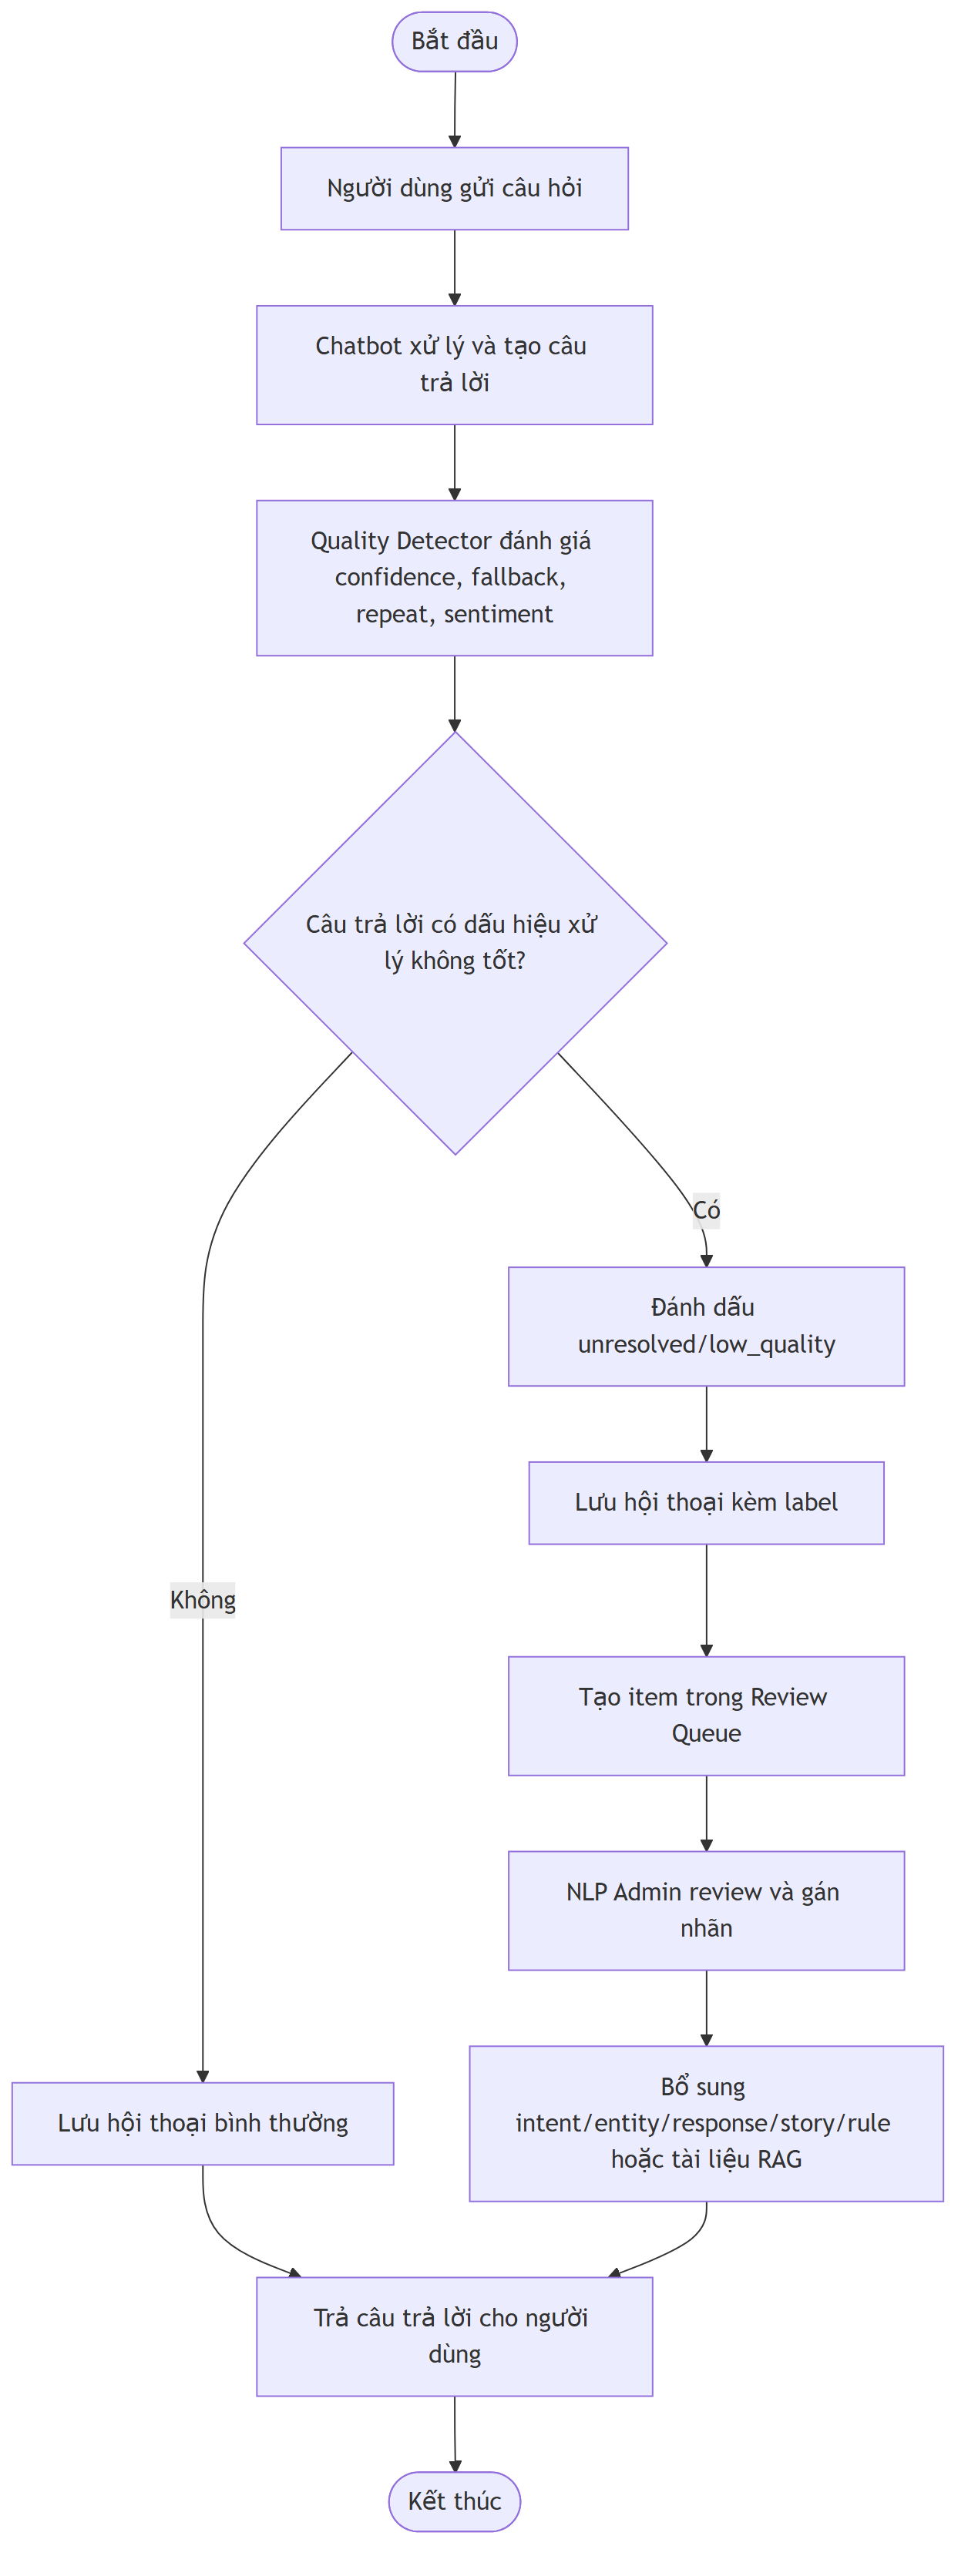
\includegraphics[width=\textwidth,height=0.78\textheight,keepaspectratio]{content/source/mermaid_activity/act_07.png}
    \caption{Activity Diagram luồng ghi nhận câu hỏi chưa xử lý tốt}
    \label{fig:act-low-quality-question-review}
\end{figure}

\begin{figure}[H]
    \centering
    \includegraphics[width=\textwidth,height=0.78\textheight,keepaspectratio]{content/source/mermaid_sequence/IMG/Luồng feedback câu trả lời để cải thiện chatbot.png}
    \caption{Sequence Diagram luồng feedback câu trả lời để cải thiện chatbot}
    \label{fig:seq-feedback-improve-chatbot}
\end{figure}

\begin{figure}[H]
    \centering
    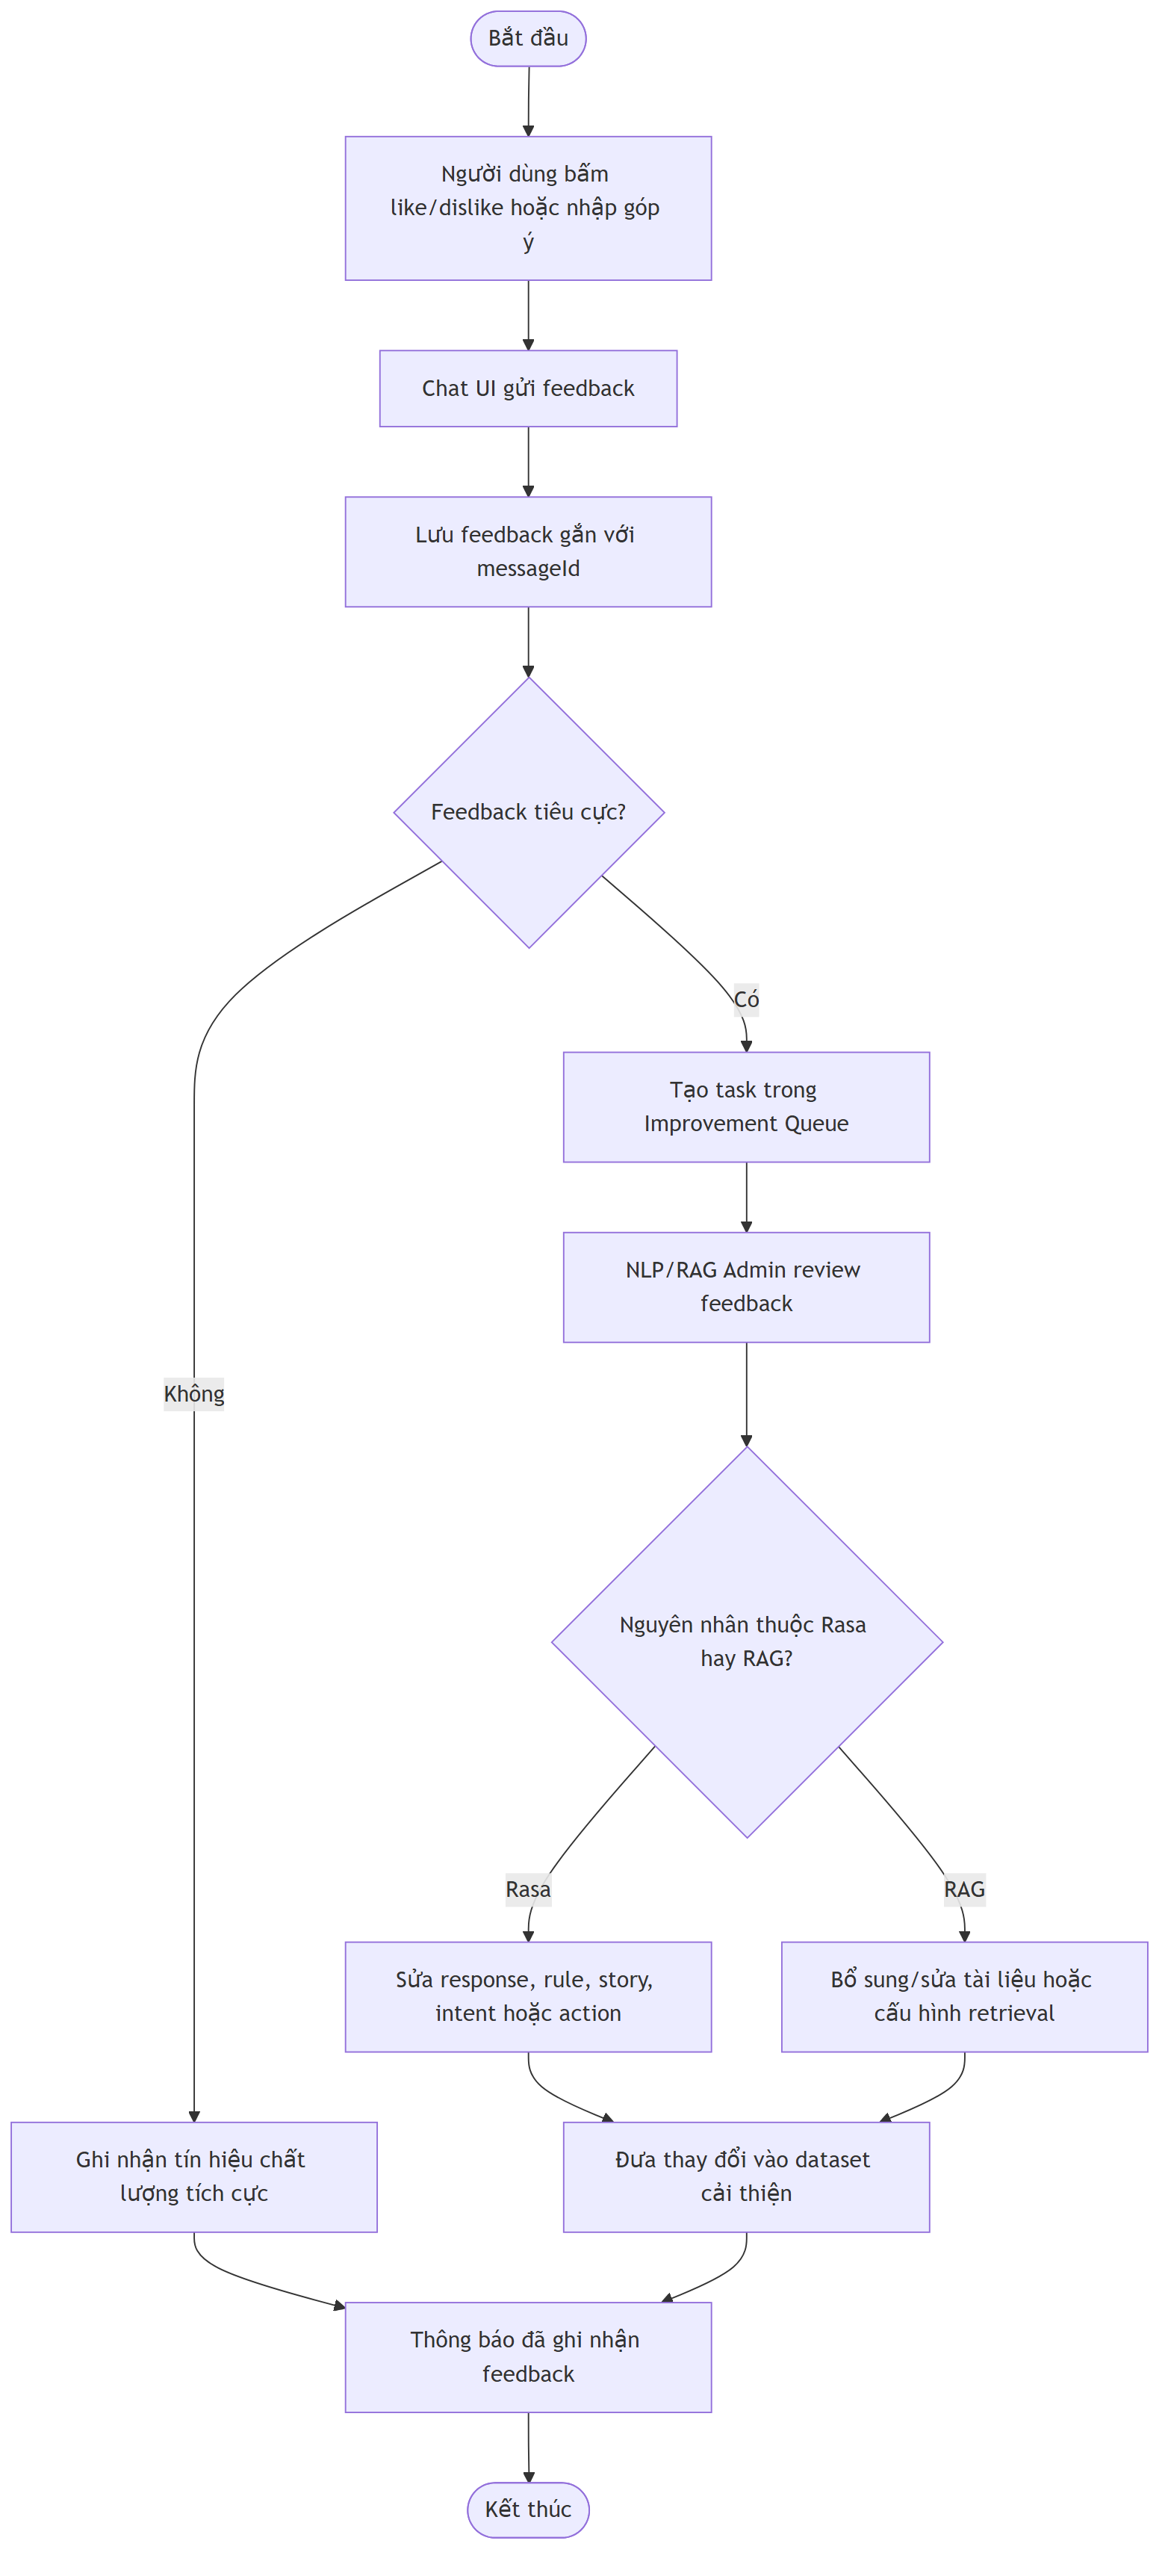
\includegraphics[width=\textwidth,height=0.78\textheight,keepaspectratio]{content/source/mermaid_activity/act_10.png}
    \caption{Activity Diagram luồng feedback câu trả lời để cải thiện chatbot}
    \label{fig:act-feedback-improve-chatbot}
\end{figure}

\section{Phân hệ RBAC và quản lý quyền}

RBAC là viết tắt của Role-Based Access Control, tức là mô hình kiểm soát truy cập dựa trên vai trò. Trong hệ thống KMA Chatbot, nhóm chức năng RBAC được thể hiện qua các route \texttt{/roles} và \texttt{/permissions}. Đây là thành phần bảo mật quan trọng vì phân hệ quản trị có nhiều thao tác ảnh hưởng trực tiếp đến dữ liệu và cấu hình hệ thống.

\subsection{Quản lý vai trò}

Màn hình \texttt{/roles} hiển thị danh sách vai trò trong hệ thống. Các vai trò đã quan sát gồm USER, MANAGER và ADMIN. Mỗi vai trò có mô tả, số lượng quyền được gán, thời điểm tạo và các thao tác quản trị.

Vai trò USER đại diện cho nhóm người dùng cơ bản với quyền truy cập hạn chế. Vai trò MANAGER đại diện cho nhóm quản lý hoặc biên tập nội dung với quyền ở mức trung bình. Vai trò ADMIN là vai trò có quyền cao nhất, có thể quản lý nhiều chức năng hệ thống.

\begin{table}[H]
\centering
\caption{Các vai trò quan sát được trong hệ thống}
\label{tab:roles-observed}
\begin{tabular}{|p{3cm}|p{6cm}|p{4cm}|}
\hline
\textbf{Vai trò} & \textbf{Mô tả} & \textbf{Mức quyền} \\ \hline
USER & Người dùng cơ bản & Thấp \\ \hline
MANAGER & Người quản lý hoặc biên tập nội dung & Trung bình \\ \hline
ADMIN & Người quản trị hệ thống & Cao \\ \hline
\end{tabular}
\end{table}

\subsection{Quản lý quyền}

Màn hình \texttt{/permissions} hiển thị danh sách quyền theo từng API hoặc chức năng. Các quyền quan sát được gồm các quyền thống kê như \texttt{GET /api/v1/statistic/system}, \texttt{GET /api/v1/statistic/documents}, \texttt{GET /api/v1/statistic/nlp}, \texttt{GET /api/v1/statistic/chatbots}, \texttt{GET /api/v1/statistic/conversations}, \texttt{GET /api/v1/statistic/users}, cùng với các quyền thao tác tài liệu như khôi phục hoặc xóa mềm tài liệu.

Cách thiết kế quyền theo endpoint giúp hệ thống kiểm soát truy cập chi tiết. Mỗi quyền gắn với một hành động cụ thể, một module cụ thể và trạng thái cho phép hay không cho phép. Khi người dùng gọi API, backend có thể kiểm tra xem vai trò của người dùng có quyền tương ứng hay không.

\subsection{Thiết kế quan hệ vai trò và quyền}

Quan hệ giữa vai trò và quyền là quan hệ nhiều-nhiều. Một vai trò có thể có nhiều quyền, và một quyền có thể được gán cho nhiều vai trò khác nhau. Vì vậy, trong cơ sở dữ liệu cần có bảng trung gian \texttt{RolePermissions} để lưu quan hệ này.

Mô hình dữ liệu đề xuất gồm:

\begin{itemize}
    \item \texttt{Roles}: lưu thông tin vai trò.
    \item \texttt{Permissions}: lưu thông tin quyền.
    \item \texttt{RolePermissions}: lưu quan hệ giữa vai trò và quyền.
    \item \texttt{Users}: lưu thông tin người dùng.
    \item \texttt{UserRoles}: lưu quan hệ giữa người dùng và vai trò.
\end{itemize}

\begin{figure}[H]
    \centering
    % \includegraphics[width=0.9\textwidth]{images/roles.png}
    \caption{Màn hình quản lý vai trò}
    \label{fig:roles-management}
\end{figure}

\begin{figure}[H]
    \centering
    % \includegraphics[width=0.9\textwidth]{images/permissions.png}
    \caption{Màn hình quản lý quyền}
    \label{fig:permissions-management}
\end{figure}

\section{Phân hệ quản lý người dùng}

Phân hệ quản lý người dùng được truy cập thông qua route \texttt{/users}. Màn hình này hiển thị danh sách tài khoản trong hệ thống với các thông tin như tên, email, ngày sinh, giới tính, trạng thái xác thực, trạng thái tài khoản và các thao tác quản trị.

Các trạng thái người dùng quan sát được gồm ACTIVE, PENDING và BANNED. Điều này cho thấy hệ thống có cơ chế quản lý vòng đời tài khoản, từ chờ duyệt, đang hoạt động đến bị cấm truy cập.

\subsection{Danh sách người dùng}

Danh sách người dùng giúp Admin theo dõi toàn bộ tài khoản đang tồn tại trong hệ thống. Các thông tin cần hiển thị gồm:

\begin{itemize}
    \item Họ tên người dùng.
    \item Email.
    \item Ngày sinh.
    \item Giới tính.
    \item Trạng thái xác thực email hoặc tài khoản.
    \item Trạng thái hoạt động.
    \item Vai trò được gán.
    \item Các thao tác quản trị.
\end{itemize}

Màn hình cần hỗ trợ tìm kiếm theo tên hoặc email, lọc theo trạng thái và phân trang để dễ quản lý khi số lượng người dùng tăng.

\subsection{Trạng thái tài khoản}

Các trạng thái tài khoản có ý nghĩa như sau:

\begin{itemize}
    \item \textbf{ACTIVE}: tài khoản đang hoạt động và có thể sử dụng hệ thống.
    \item \textbf{PENDING}: tài khoản đang chờ xác nhận hoặc chờ duyệt.
    \item \textbf{BANNED}: tài khoản bị cấm hoặc bị khóa quyền truy cập.
\end{itemize}

Việc phân biệt trạng thái giúp Admin kiểm soát truy cập tốt hơn. Ví dụ, tài khoản PENDING có thể chưa được phép truy cập đầy đủ, còn tài khoản BANNED cần bị chặn đăng nhập hoặc chặn thao tác trong hệ thống.

\subsection{Thao tác quản trị người dùng}

Các thao tác quản trị người dùng cần có gồm:

\begin{itemize}
    \item Tạo tài khoản mới.
    \item Cập nhật thông tin tài khoản.
    \item Gán hoặc thay đổi vai trò.
    \item Khóa hoặc mở khóa tài khoản.
    \item Đặt lại mật khẩu nếu cần.
    \item Xóa mềm tài khoản.
\end{itemize}

Mọi thao tác quan trọng trên tài khoản cần được ghi log để phục vụ truy vết. Đặc biệt, các thao tác như gán quyền Admin, khóa tài khoản hoặc xóa tài khoản cần yêu cầu quyền cao và có hộp thoại xác nhận.

\begin{figure}[H]
    \centering
    % \includegraphics[width=0.9\textwidth]{images/users.png}
    \caption{Màn hình quản lý người dùng}
    \label{fig:users-management}
\end{figure}

\section{Thiết kế luồng nghiệp vụ phân hệ quản trị}

\subsection{Luồng quản lý tài liệu biểu mẫu}

Luồng quản lý tài liệu biểu mẫu bắt đầu khi Admin hoặc Manager cần thêm mới hoặc cập nhật một biểu mẫu. Người quản trị truy cập màn hình \texttt{/docs}, tải file lên, nhập mô tả, gán tag và lưu thông tin. Backend kiểm tra định dạng file, lưu metadata và cập nhật danh sách tài liệu.

Quy trình gồm:

\begin{enumerate}
    \item Người quản trị đăng nhập hệ thống.
    \item Truy cập màn hình Documents.
    \item Thêm mới hoặc chỉnh sửa tài liệu.
    \item Nhập tên, mô tả, tag và chọn file.
    \item Backend kiểm tra dữ liệu.
    \item File và metadata được lưu vào hệ thống.
    \item Giao diện cập nhật danh sách tài liệu.
\end{enumerate}

\subsection{Luồng quản lý tài liệu RAG}

Luồng quản lý tài liệu RAG bắt đầu từ màn hình \texttt{/context-docs}. Người quản trị upload tài liệu hoặc scan tài liệu mới. Sau đó pipeline xử lý tài liệu, sinh chunks và cập nhật trạng thái.

Quy trình gồm:

\begin{enumerate}
    \item Người quản trị chọn chatbot cần thao tác.
    \item Truy cập màn hình Context Documents.
    \item Upload tài liệu hoặc scan tài liệu mới.
    \item Hệ thống đưa tài liệu vào pipeline xử lý.
    \item Pipeline trích xuất văn bản, chia chunks và sinh embedding.
    \item Trạng thái tài liệu được cập nhật thành processed hoặc failed.
    \item Nếu failed, người quản trị có thể retry pipeline.
\end{enumerate}

\subsection{Luồng phân quyền người dùng}

Luồng phân quyền bắt đầu khi Admin cần cấp quyền cho một nhóm người dùng. Admin tạo hoặc cập nhật vai trò, sau đó gán các quyền cần thiết cho vai trò đó. Cuối cùng, Admin gán vai trò cho tài khoản người dùng.

Quy trình gồm:

\begin{enumerate}
    \item Admin truy cập màn hình Roles.
    \item Tạo hoặc chỉnh sửa vai trò.
    \item Chọn danh sách quyền từ màn hình Permissions.
    \item Gán quyền cho vai trò.
    \item Truy cập màn hình Users.
    \item Gán vai trò cho người dùng.
    \item Backend áp dụng kiểm tra quyền khi người dùng truy cập API.
\end{enumerate}

\begin{figure}[H]
    \centering
    \includegraphics[width=\textwidth,height=0.78\textheight,keepaspectratio]{content/source/mermaid_sequence/IMG/Luồng phân quyền RBAC.png}
    \caption{Sequence Diagram luồng phân quyền RBAC}
    \label{fig:seq-rbac-authorization}
\end{figure}

\begin{figure}[H]
    \centering
    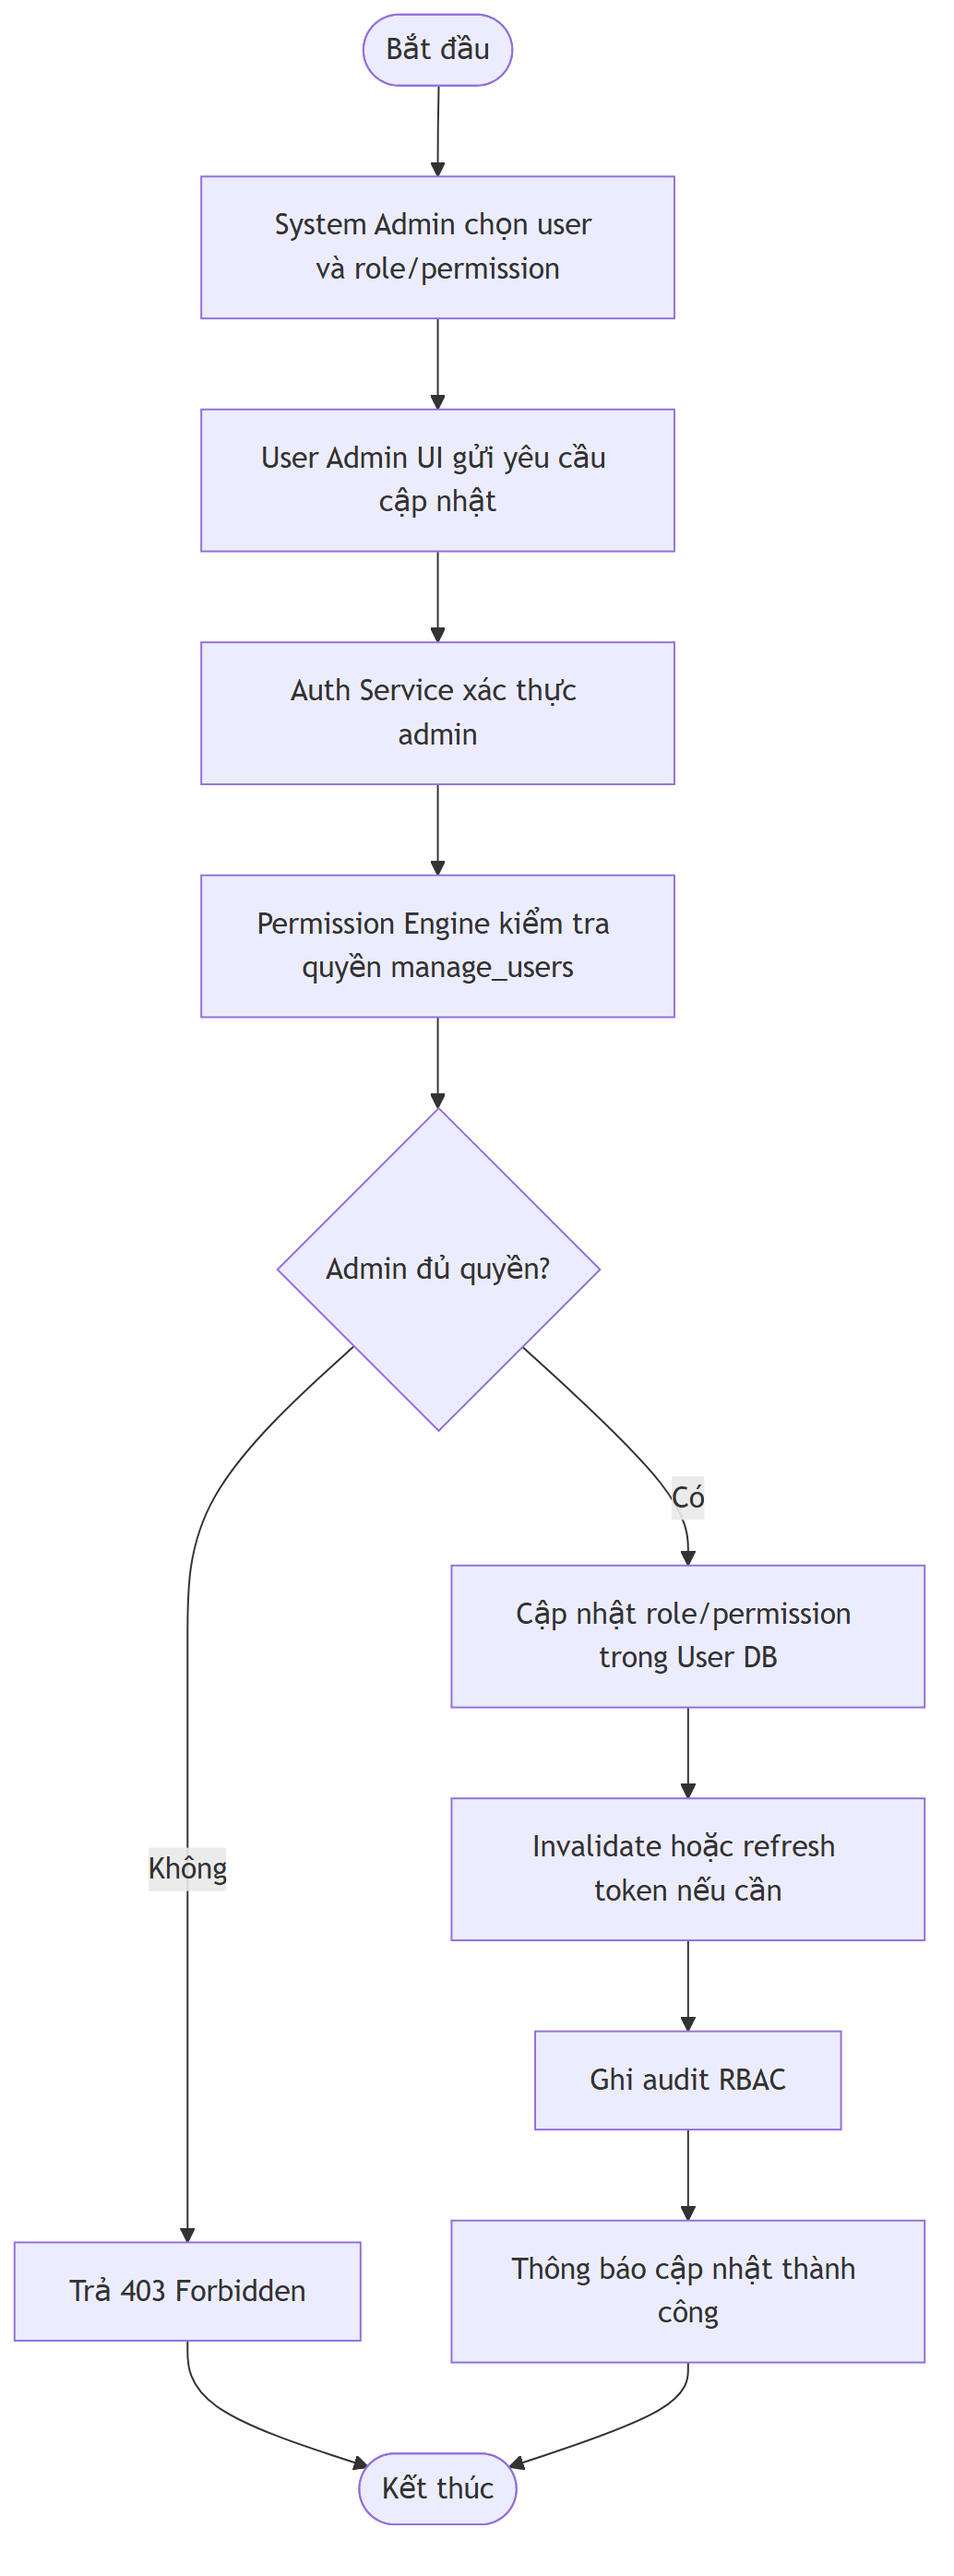
\includegraphics[width=\textwidth,height=0.78\textheight,keepaspectratio]{content/source/mermaid_activity/act_09.png}
    \caption{Activity Diagram luồng phân quyền RBAC}
    \label{fig:act-rbac-authorization}
\end{figure}

\subsection{Luồng xem báo cáo thống kê}

Luồng xem báo cáo thống kê cho phép Admin hoặc Manager theo dõi tình trạng hệ thống theo từng nhóm dữ liệu.

Quy trình gồm:

\begin{enumerate}
    \item Người quản trị chọn chatbot cần xem báo cáo.
    \item Truy cập nhóm Statistics.
    \item Chọn loại báo cáo: Users, Conversations, Chatbots hoặc Documents.
    \item Frontend gọi API thống kê tương ứng.
    \item Backend tổng hợp dữ liệu.
    \item Giao diện hiển thị số liệu, biểu đồ và bảng chi tiết.
\end{enumerate}

\section{Thiết kế cơ sở dữ liệu phục vụ phân hệ quản trị}

Để hỗ trợ phân hệ quản trị, hệ thống cần tổ chức các nhóm bảng dữ liệu phục vụ người dùng, vai trò, quyền, tài liệu, tài liệu RAG, chatbot và thống kê.

\begin{table}[H]
\centering
\caption{Các bảng dữ liệu đề xuất cho phân hệ quản trị}
\label{tab:admin-db}
\begin{tabular}{|p{4cm}|p{5cm}|p{6cm}|}
\hline
\textbf{Nhóm dữ liệu} & \textbf{Bảng đề xuất} & \textbf{Mục đích} \\ \hline
Người dùng & \texttt{Users} & Lưu thông tin tài khoản người dùng \\ \hline
Vai trò & \texttt{Roles} & Lưu danh sách vai trò trong hệ thống \\ \hline
Quyền & \texttt{Permissions} & Lưu danh sách quyền theo module hoặc endpoint \\ \hline
Người dùng -- vai trò & \texttt{UserRoles} & Gán vai trò cho người dùng \\ \hline
Vai trò -- quyền & \texttt{RolePermissions} & Gán quyền cho vai trò \\ \hline
Chatbot & \texttt{Chatbots} & Lưu thông tin chatbot và trạng thái hoạt động \\ \hline
Tài liệu biểu mẫu & \texttt{Documents} & Lưu thông tin tài liệu, biểu mẫu \\ \hline
Tag tài liệu & \texttt{DocumentTags} & Phân loại tài liệu theo tag \\ \hline
Tài liệu RAG & \texttt{ContextDocuments} & Lưu tài liệu ngữ cảnh phục vụ RAG \\ \hline
Chunks & \texttt{DocumentChunks} & Lưu các đoạn văn bản sau khi chia nhỏ \\ \hline
Trạng thái pipeline & \texttt{PipelineLogs} & Lưu trạng thái và lỗi xử lý tài liệu \\ \hline
Hội thoại & \texttt{Conversations} & Lưu phiên hội thoại của người dùng \\ \hline
Tin nhắn & \texttt{Messages} & Lưu câu hỏi và câu trả lời \\ \hline
Thống kê & \texttt{StatisticSnapshots} & Lưu số liệu thống kê theo thời gian nếu cần \\ \hline
Nhật ký thao tác & \texttt{AuditLogs} & Lưu lịch sử thao tác quản trị \\ \hline
\end{tabular}
\end{table}

Quan hệ dữ liệu cơ bản được mô tả như sau: một người dùng có thể có nhiều vai trò, một vai trò có thể có nhiều quyền, một chatbot có thể có nhiều tài liệu, một tài liệu RAG có thể sinh ra nhiều chunks, một hội thoại có thể có nhiều tin nhắn và mỗi thao tác quản trị quan trọng cần được ghi vào audit log.

\section{Yêu cầu bảo mật và kiểm soát truy cập}

Phân hệ quản trị có quyền thay đổi dữ liệu quan trọng của hệ thống, do đó cần thiết kế bảo mật chặt chẽ. Các yêu cầu bảo mật chính gồm:

\begin{itemize}
    \item Người dùng phải đăng nhập trước khi truy cập khu vực quản trị.
    \item Backend phải kiểm tra token hợp lệ đối với mọi API quản trị.
    \item Mỗi API cần được gắn với quyền cụ thể.
    \item Người dùng chỉ được thao tác nếu vai trò của họ có quyền tương ứng.
    \item Các thao tác quan trọng như xóa mềm, khôi phục, thay đổi quyền cần ghi audit log.
    \item Thông tin nhạy cảm như token, secret key hoặc API key không được hiển thị trực tiếp trên giao diện.
    \item Tài khoản BANNED không được phép đăng nhập hoặc thao tác.
    \item Tài khoản PENDING cần bị giới hạn quyền cho đến khi được duyệt.
    \item Cần có cơ chế chống truy cập trái phép vào các route như \texttt{/roles}, \texttt{/permissions} và \texttt{/users}.
\end{itemize}

Mô hình RBAC giúp hệ thống kiểm soát truy cập theo vai trò thay vì kiểm tra thủ công từng người dùng. Điều này giúp hệ thống dễ mở rộng và dễ quản lý hơn khi số lượng tài khoản tăng.

\section{Yêu cầu giao diện người dùng}

Giao diện quản trị cần đảm bảo dễ sử dụng, rõ ràng và phù hợp với người quản trị nội dung không chuyên sâu kỹ thuật. Các màn hình cần thống nhất về bố cục, màu sắc, vị trí nút thao tác và cách hiển thị trạng thái.

Các yêu cầu giao diện gồm:

\begin{itemize}
    \item Có sidebar để truy cập nhanh đến các nhóm chức năng.
    \item Có trường chọn chatbot để khoanh vùng dữ liệu quản trị.
    \item Các bảng dữ liệu cần hỗ trợ tìm kiếm, lọc và phân trang.
    \item Trạng thái tài liệu cần hiển thị bằng nhãn dễ nhận biết.
    \item Các thao tác nguy hiểm như xóa cần có hộp thoại xác nhận.
    \item Màn hình thống kê cần có thẻ số liệu tổng quan và biểu đồ trực quan.
    \item Màn hình context documents cần hiển thị trạng thái pipeline rõ ràng.
    \item Màn hình roles và permissions cần cho phép xem nhanh số quyền, module và endpoint.
    \item Màn hình users cần hiển thị trạng thái tài khoản rõ ràng như ACTIVE, PENDING, BANNED.
\end{itemize}

\section{Đánh giá hiện trạng phân hệ quản trị}

Dựa trên giao diện đã quan sát, phân hệ quản trị của hệ thống KMA Chatbot đã có các nhóm chức năng nền tảng để vận hành hệ thống chatbot tuyển sinh. Các chức năng quản lý tài liệu, quản lý tài liệu ngữ cảnh, thống kê, RBAC và quản lý người dùng đã được thể hiện rõ qua UI.

\subsection{Điểm mạnh}

Các điểm mạnh của phân hệ quản trị gồm:

\begin{itemize}
    \item Có màn hình quản lý tài liệu và biểu mẫu riêng.
    \item Có màn hình quản lý tài liệu ngữ cảnh phục vụ RAG.
    \item Có cơ chế scan, upload, retry pipeline và lọc trạng thái tài liệu.
    \item Có trường chọn chatbot trên nhiều màn hình, hỗ trợ quản trị theo ngữ cảnh chatbot.
    \item Có nhóm báo cáo thống kê cho người dùng, hội thoại, chatbot và tài liệu.
    \item Có RBAC với vai trò và quyền chi tiết theo endpoint.
    \item Có màn hình quản lý người dùng với nhiều trạng thái tài khoản.
    \item Có dấu hiệu hỗ trợ xóa mềm và khôi phục tài liệu.
\end{itemize}

\subsection{Hạn chế}

Một số hạn chế hoặc điểm cần kiểm tra thêm gồm:

\begin{itemize}
    \item Chưa xác minh được màn hình tạo, sửa, xóa chatbot riêng biệt.
    \item Route thống kê NLP chưa tải được trong phiên quan sát hiện tại.
    \item Cần bổ sung thống kê chất lượng RAG như tỷ lệ câu trả lời có citation, tài liệu được truy hồi nhiều nhất và câu hỏi không tìm thấy nguồn.
    \item Cần kiểm tra kỹ cơ chế phân quyền thực tế khi người dùng không đủ quyền truy cập route quản trị.
    \item Cần bổ sung audit log rõ ràng cho các thao tác quan trọng.
\end{itemize}

\section{Định hướng hoàn thiện phân hệ quản trị}

Để phân hệ quản trị hoàn thiện hơn, hệ thống có thể phát triển thêm các nhóm chức năng sau:

\begin{itemize}
    \item Bổ sung màn hình quản lý chatbot đầy đủ nếu hệ thống định hướng hỗ trợ nhiều chatbot.
    \item Hoàn thiện màn hình thống kê NLP và RAG.
    \item Bổ sung dashboard chất lượng RAG với các chỉ số về retrieval, citation và feedback.
    \item Bổ sung quy trình duyệt tài liệu trước khi đưa vào kho tri thức.
    \item Tách rõ vai trò người quản trị hệ thống, người quản trị nội dung và người duyệt tài liệu.
    \item Bổ sung lịch sử phiên bản tài liệu để phục hồi khi cập nhật sai.
    \item Chuẩn hóa tên file, encoding tiếng Việt và metadata tài liệu.
    \item Bổ sung bộ kiểm thử định kỳ cho các câu hỏi tuyển sinh trọng yếu.
\end{itemize}

\section{Kết luận chương}

Chương này đã trình bày phân tích và thiết kế phân hệ quản trị của hệ thống KMA Chatbot tuyển sinh dựa trên giao diện UI đã quan sát. Phân hệ quản trị bao gồm các nhóm chức năng chính như quản lý tài liệu và biểu mẫu, quản lý tài liệu ngữ cảnh RAG, quản lý chatbot theo ngữ cảnh, báo cáo thống kê, RBAC và quản lý người dùng.

Thông qua phân hệ quản trị, Admin và người quản trị nội dung có thể cập nhật tài liệu, theo dõi trạng thái xử lý RAG, kiểm soát người dùng, phân quyền truy cập và đánh giá tình trạng vận hành của chatbot. Đây là nền tảng quan trọng giúp hệ thống có khả năng vận hành thực tế, mở rộng theo nhiều chatbot và cải thiện chất lượng tư vấn tuyển sinh dựa trên dữ liệu được quản lý tập trung.

Mặc dù một số chức năng như thống kê NLP hoặc CRUD chatbot riêng biệt chưa được xác minh đầy đủ trong phiên quan sát hiện tại, hệ thống đã thể hiện rõ kiến trúc quản trị cần thiết cho một chatbot tư vấn tuyển sinh có tích hợp Rasa và RAG. Trong các giai đoạn tiếp theo, trọng tâm cần tập trung vào hoàn thiện thống kê chất lượng NLP/RAG, kiểm soát pipeline tài liệu, bổ sung audit log và tăng cường phân quyền chi tiết theo vai trò.


\endgroup

% 
\chapter{XÂY DỰNG}
\label{chap:implementation}



\clearpage
\chapter*{KẾT LUẬN}
\phantomsection
\addcontentsline{toc}{chapter}{KẾT LUẬN}

Báo cáo đã trình bày toàn bộ quá trình phân tích kỹ thuật cho hệ thống trợ lý ảo tư vấn tuyển sinh KMA theo hai hướng chính: chatbot hội thoại dựa trên Rasa và phân hệ truy xuất tri thức dựa trên KmaRAG. Ở phía chatbot, tài liệu đã làm rõ kiến trúc frontend, backend Node.js, Flask bridge, Rasa Server, Action Server, cơ chế phân loại intent bằng PhoBERT, quản lý hội thoại, fallback và quy trình huấn luyện mô hình. Ở phía RAG, báo cáo đã mô tả kiến trúc nhiều lớp, các pipeline ingest và query, lớp lưu trữ đa tầng, cơ chế xây dựng knowledge graph, truy hồi ngữ nghĩa, xây dựng context và sinh câu trả lời có nguồn tham chiếu.

Kết quả phân tích cho thấy hệ thống được thiết kế theo hướng tách lớp rõ ràng, có khả năng mở rộng, dễ bảo trì và phù hợp với bài toán tư vấn tuyển sinh thực tế. Việc kết hợp giữa luồng hội thoại có kiểm soát của Rasa và luồng truy xuất tri thức động của KmaRAG giúp hệ thống vừa đảm bảo tính ổn định cho các câu hỏi phổ biến, vừa tăng khả năng trả lời các câu hỏi mở dựa trên tài liệu nghiệp vụ. Đây là nền tảng phù hợp để tiếp tục phát triển các chức năng như nâng cao chất lượng retrieval, tối ưu citation, mở rộng tập tri thức, tăng cường đánh giá chất lượng phản hồi và hỗ trợ vận hành ở quy mô lớn hơn.

\clearpage
\chapter*{TÀI LIỆU THAM KHẢO}
\phantomsection
\addcontentsline{toc}{chapter}{TÀI LIỆU THAM KHẢO}

\begingroup
\footnotesize
\renewcommand{\baselinestretch}{1.0}\selectfont
\setlength{\parskip}{0pt}
\setlength{\itemsep}{1pt}
\setlength{\parsep}{0pt}
\setlength{\topsep}{2pt}
\begin{enumerate}[leftmargin=1.2cm,label={[\arabic*]},itemsep=1pt,topsep=2pt]
\item Rasa Technologies, \textit{Rasa Open Source Documentation}, \url{https://rasa.com/docs/rasa/}.
\item D. Q. Nguyen, A. T. Nguyen, \textit{PhoBERT: Pre-trained language models for Vietnamese}, Findings of EMNLP 2020.
\item Qdrant, \textit{Qdrant Documentation}, \url{https://qdrant.tech/documentation/}.
\item Redis, \textit{Redis Documentation}, \url{https://redis.io/docs/}.
\item Memgraph, \textit{Memgraph Documentation}, \url{https://memgraph.com/docs}.
\item Mã nguồn và tài liệu kỹ thuật nội bộ của các phân hệ \texttt{kmarag-main}, \texttt{rasa\_flask\_api}, \texttt{rasa\_m\_be}, \texttt{rasa\_fe}.
\item Tài liệu tuyển sinh, tài liệu nghiệp vụ, biểu mẫu và dữ liệu vận hành nội bộ dùng để xây dựng tập tri thức của hệ thống.
\end{enumerate}
\endgroup



\end{document}

